%Version 3.1 December 2024
% See section 11 of the User Manual for version history
%
%%%%%%%%%%%%%%%%%%%%%%%%%%%%%%%%%%%%%%%%%%%%%%%%%%%%%%%%%%%%%%%%%%%%%%
%%                                                                 %%
%% Please do not use \input{...} to include other tex files.       %%
%% Submit your LaTeX manuscript as one .tex document.              %%
%%                                                                 %%
%% All additional figures and files should be attached             %%
%% separately and not embedded in the \TeX\ document itself.       %%
%%                                                                 %%
%%%%%%%%%%%%%%%%%%%%%%%%%%%%%%%%%%%%%%%%%%%%%%%%%%%%%%%%%%%%%%%%%%%%%

%%\documentclass[referee,sn-basic]{sn-jnl}% referee option is meant for double line spacing

%%=======================================================%%
%% to print line numbers in the margin use lineno option %%
%%=======================================================%%

%%\documentclass[lineno,pdflatex,sn-basic]{sn-jnl}% Basic Springer Nature Reference Style/Chemistry Reference Style

%%=========================================================================================%%
%% the documentclass is set to pdflatex as default. You can delete it if not appropriate.  %%
%%=========================================================================================%%

%%\documentclass[sn-basic]{sn-jnl}% Basic Springer Nature Reference Style/Chemistry Reference Style

%%Note: the following reference styles support Namedate and Numbered referencing. By default the style follows the most common style. To switch between the options you can add or remove “Numbered” in the optional parenthesis. 
%%The option is available for: sn-basic.bst, sn-chicago.bst%  
 
\documentclass[pdflatex,sn-nature]{sn-jnl}% Style for submissions to Nature Portfolio journals
%%\documentclass[pdflatex,sn-basic]{sn-jnl}% Basic Springer Nature Reference Style/Chemistry Reference Style
%\documentclass[pdflatex,sn-mathphys-num]{sn-jnl}% Math and Physical Sciences Numbered Reference Style
%%\documentclass[pdflatex,sn-mathphys-ay]{sn-jnl}% Math and Physical Sciences Author Year Reference Style
%%\documentclass[pdflatex,sn-aps]{sn-jnl}% American Physical Society (APS) Reference Style
%%\documentclass[pdflatex,sn-vancouver-num]{sn-jnl}% Vancouver Numbered Reference Style
%%\documentclass[pdflatex,sn-vancouver-ay]{sn-jnl}% Vancouver Author Year Reference Style
%%\documentclass[pdflatex,sn-apa]{sn-jnl}% APA Reference Style
%%\documentclass[pdflatex,sn-chicago]{sn-jnl}% Chicago-based Humanities Reference Style

%%%% Standard Packages
%%<additional latex packages if required can be included here>

\usepackage{graphicx}%
\usepackage{multirow}%
\usepackage{amsmath,amssymb,amsfonts}%
\usepackage{amsthm}%
\usepackage{mathrsfs}%
\usepackage[title]{appendix}%
\usepackage{xcolor}%
\usepackage{textcomp}%
\usepackage{manyfoot}%
\usepackage{booktabs}%
\usepackage{algorithm}%
\usepackage{algorithmicx}%
\usepackage{algpseudocode}%
\usepackage{listings}%



%%%%%%%%%%%%%%%%%%%%%%%%%%%
%\usepackage{bm}
\usepackage{braket}
\usepackage{tikz}
\usepackage{fontawesome}
\usetikzlibrary{arrows.meta,positioning,fit,calc,shapes.symbols,shapes.misc}


\usepackage{booktabs}
\usepackage{array}
\usepackage{makecell}
\usepackage{arydshln} % provides dashed vertical rules via ':' in the preamble

\newcolumntype{R}{>{$}r<{$}} % right-aligned, math mode
\newcolumntype{L}{>{$}l<{$}} % left-aligned,  math mode
\newcommand{\tup}[1]{\left(#1\right)}

% optional: tune dashed rule look
\setlength\dashlinedash{0.6pt}
\setlength\dashlinegap{1.3pt}




%%%%

%%%%%=============================================================================%%%%
%%%%  Remarks: This template is provided to aid authors with the preparation
%%%%  of original research articles intended for submission to journals published 
%%%%  by Springer Nature. The guidance has been prepared in partnership with 
%%%%  production teams to conform to Springer Nature technical requirements. 
%%%%  Editorial and presentation requirements differ among journal portfolios and 
%%%%  research disciplines. You may find sections in this template are irrelevant 
%%%%  to your work and are empowered to omit any such section if allowed by the 
%%%%  journal you intend to submit to. The submission guidelines and policies 
%%%%  of the journal take precedence. A detailed User Manual is available in the 
%%%%  template package for technical guidance.
%%%%%=============================================================================%%%%

%% as per the requirement new theorem styles can be included as shown below
\theoremstyle{thmstyleone}%
\newtheorem{theorem}{Theorem}%  meant for continuous numbers
%%\newtheorem{theorem}{Theorem}[section]% meant for sectionwise numbers
%% optional argument [theorem] produces theorem numbering sequence instead of independent numbers for Proposition
\newtheorem{proposition}[theorem]{Proposition}% 
%%\newtheorem{proposition}{Proposition}% to get separate numbers for theorem and proposition etc.

\theoremstyle{thmstyletwo}%
\newtheorem{example}{Example}%
\newtheorem{remark}{Remark}%

\theoremstyle{thmstylethree}%
\newtheorem{definition}{Definition}%

\raggedbottom
%%\unnumbered% uncomment this for unnumbered level heads

\begin{document}


\title[]{Co-Designing Quantum Codes with Transversal Diagonal Gates via Multi-Agent Systems}

%%=============================================================%%
%% GivenName	-> \fnm{Joergen W.}
%% Particle	-> \spfx{van der} -> surname prefix
%% FamilyName	-> \sur{Ploeg}
%% Suffix	-> \sfx{IV}
%% \author*[1,2]{\fnm{Joergen W.} \spfx{van der} \sur{Ploeg} 
%%  \sfx{IV}}\email{iauthor@gmail.com}
%%=============================================================%%

\author[1]{\fnm{Xi} \sur{He}}%\email{iauthor@gmail.com}

\author[2]{\fnm{Sirui} \sur{Lu}}%\email{iiauthor@gmail.com}
%\equalcont{These authors contributed equally to this work.}

\author*[1]{\fnm{Bei} \sur{Zeng}}\email{bei.zeng@utdallas.edu}
%\equalcont{These authors contributed equally to this work.}

\affil[1]{\orgdiv{Department of Physics}, \orgname{The University of Texas at Dallas}, \orgaddress{\city{Richardson}, \state{Texas}, \postcode{75080}, \country{USA}}}

\affil[2]{\orgname{Max-Planck-Institut f\"ur Quantenoptik}, \orgaddress{\city{Garching bei M\"unchen}, \postcode{85748}, \country{Germany}}}


%\affil[3]{\orgdiv{Department}, \orgname{Organization}, \orgaddress{\street{Street}, \city{City}, \postcode{610101}, \state{State}, \country{Country}}}

%%==================================%%
%% Sample for unstructured abstract %%
%%==================================%%

\abstract{
We present a multi-agent, human-in-the-loop workflow that co-designs quantum error-correcting codes with prescribed transversal diagonal gates. It builds on the Subset-Sum Linear Programming (SSLP) framework, which partitions basis strings by modular residues and enforces Z-marginal Knill--Laflamme (KL) equalities via small LPs. The workflow is powered by GPT-5 and implemented within TeXRA, a multi-agent research assistant platform where agents collaborate in a shared \LaTeX--Python workspace synchronized with Git/Overleaf. Three specialized agents formulate constraints, sweep and screen candidate codes, exactify numerical solutions into rationals, and independently audit all KL equalities and induced logical actions. Focusing on distance-two codes with nondegenerate residues, we catalogue new nonadditive codes for dimensions $K\in\{2,3,4\}$ on up to six qubits, including high-order diagonal transversals, yielding $14,116$ new codes. From these data, the system abstracts closed-form families and constructs a residue-degenerate $((6,4,2))$ code implementing a transversal controlled-phase $\mathrm{diag}(1,1,1,i)$, illustrating how AI orchestration can drive rigorous, scalable code discovery.
}

% 


%%================================%%
%% Sample for structured abstract %%
%%================================%%

% \abstract{\textbf{Purpose:} The abstract serves both as a general introduction to the topic and as a brief, non-technical summary of the main results and their implications. The abstract must not include subheadings (unless expressly permitted in the journal's Instructions to Authors), equations or citations. As a guide the abstract should not exceed 200 words. Most journals do not set a hard limit however authors are advised to check the author instructions for the journal they are submitting to.
% 
% \textbf{Methods:} The abstract serves both as a general introduction to the topic and as a brief, non-technical summary of the main results and their implications. The abstract must not include subheadings (unless expressly permitted in the journal's Instructions to Authors), equations or citations. As a guide the abstract should not exceed 200 words. Most journals do not set a hard limit however authors are advised to check the author instructions for the journal they are submitting to.
% 
% \textbf{Results:} The abstract serves both as a general introduction to the topic and as a brief, non-technical summary of the main results and their implications. The abstract must not include subheadings (unless expressly permitted in the journal's Instructions to Authors), equations or citations. As a guide the abstract should not exceed 200 words. Most journals do not set a hard limit however authors are advised to check the author instructions for the journal they are submitting to.
% 
% \textbf{Conclusion:} The abstract serves both as a general introduction to the topic and as a brief, non-technical summary of the main results and their implications. The abstract must not include subheadings (unless expressly permitted in the journal's Instructions to Authors), equations or citations. As a guide the abstract should not exceed 200 words. Most journals do not set a hard limit however authors are advised to check the author instructions for the journal they are submitting to.}

\keywords{Quantum error-correcting codes, Transversal diagonal gates, Multi-agent large language models, AI-assisted scientific discovery}

%%\pacs[JEL Classification]{D8, H51}

%%\pacs[MSC Classification]{35A01, 65L10, 65L12, 65L20, 65L70}

\maketitle

\section{Introduction}
\label{sec:intro}

AI systems are increasingly taking on novel research tasks~\cite{Wang2023Scientific,Lu2024AI,Binz2025How,Glazer2024FrontierMath,Lu2025Can}, yet face challenges beyond current capabilities. Success requires identifying problems with the right structure: those requiring large-scale exploration of combinatorial search spaces where solutions are hard to generate but easy to verify. In mathematics and physics, many seminal solutions were obtained by hand-constructing candidate solutions, guided by intuition and checked against constraints. While human intuition excels at proposing such candidates, large-scale enumeration and pattern extraction remain bottlenecks. AI systems have long excelled at search and optimization, from game playing~\cite{Silver2016Mastering,Silver2017Mastering} and protein structure prediction~\cite{Jumper2021Highly} to automated theorem proving~\cite{Romera-Paredes2024Mathematical,Trinh2024Solving}. Large language models~\cite{Brown2020Language} add complementary capabilities: tool-use~\cite{Schick2023Toolformer,Anthropic2024Model,Patil2023Gorilla} (generating and executing domain code~\cite{Tian2024SciCode,Jimenez2024SWEbench}) and reasoning (deriving analytical theories from examples~\cite{OpenAI2024OpenAI,Guo2025DeepSeekR1}), though current systems still require substantial human supervision.

We implement a multi-agent system~\cite{Wu2023AutoGen,Du2023Improving,Sumers2023Cognitive} and apply it to discover novel quantum error-correcting codes. The system is built around TeXRA~\cite{Texra2025TeXRA}, an agentic AI research assistant with GPT-5~\cite{Openai2025GPT} that enables file creation, code execution, and natural-language interaction within a working directory containing \LaTeX{} formulations, Python code, and results. The working directory can be connected as a git repository to Overleaf for sharing among collaborators. The platform supports two operational modes: a \emph{tool-use loop}~\cite{Yao2023ReAct} where agents iteratively call functions for writing code, executing searches, processing data; a \emph{derivation-then-edit workflow} where agents expand mathematical derivations in an internal scratchpad, then produce edited LaTeX files for human review. Three specialized agents operate under human orchestration in this shared environment (Fig.~\ref{fig1:sche}), combining tool-use and reasoning to address a feasibility-and-construction problem in quantum error correction: determining which transversal gate groups can arise for quantum codes with specified physical and logical parameters.

\begin{figure}[t]
    \centering
    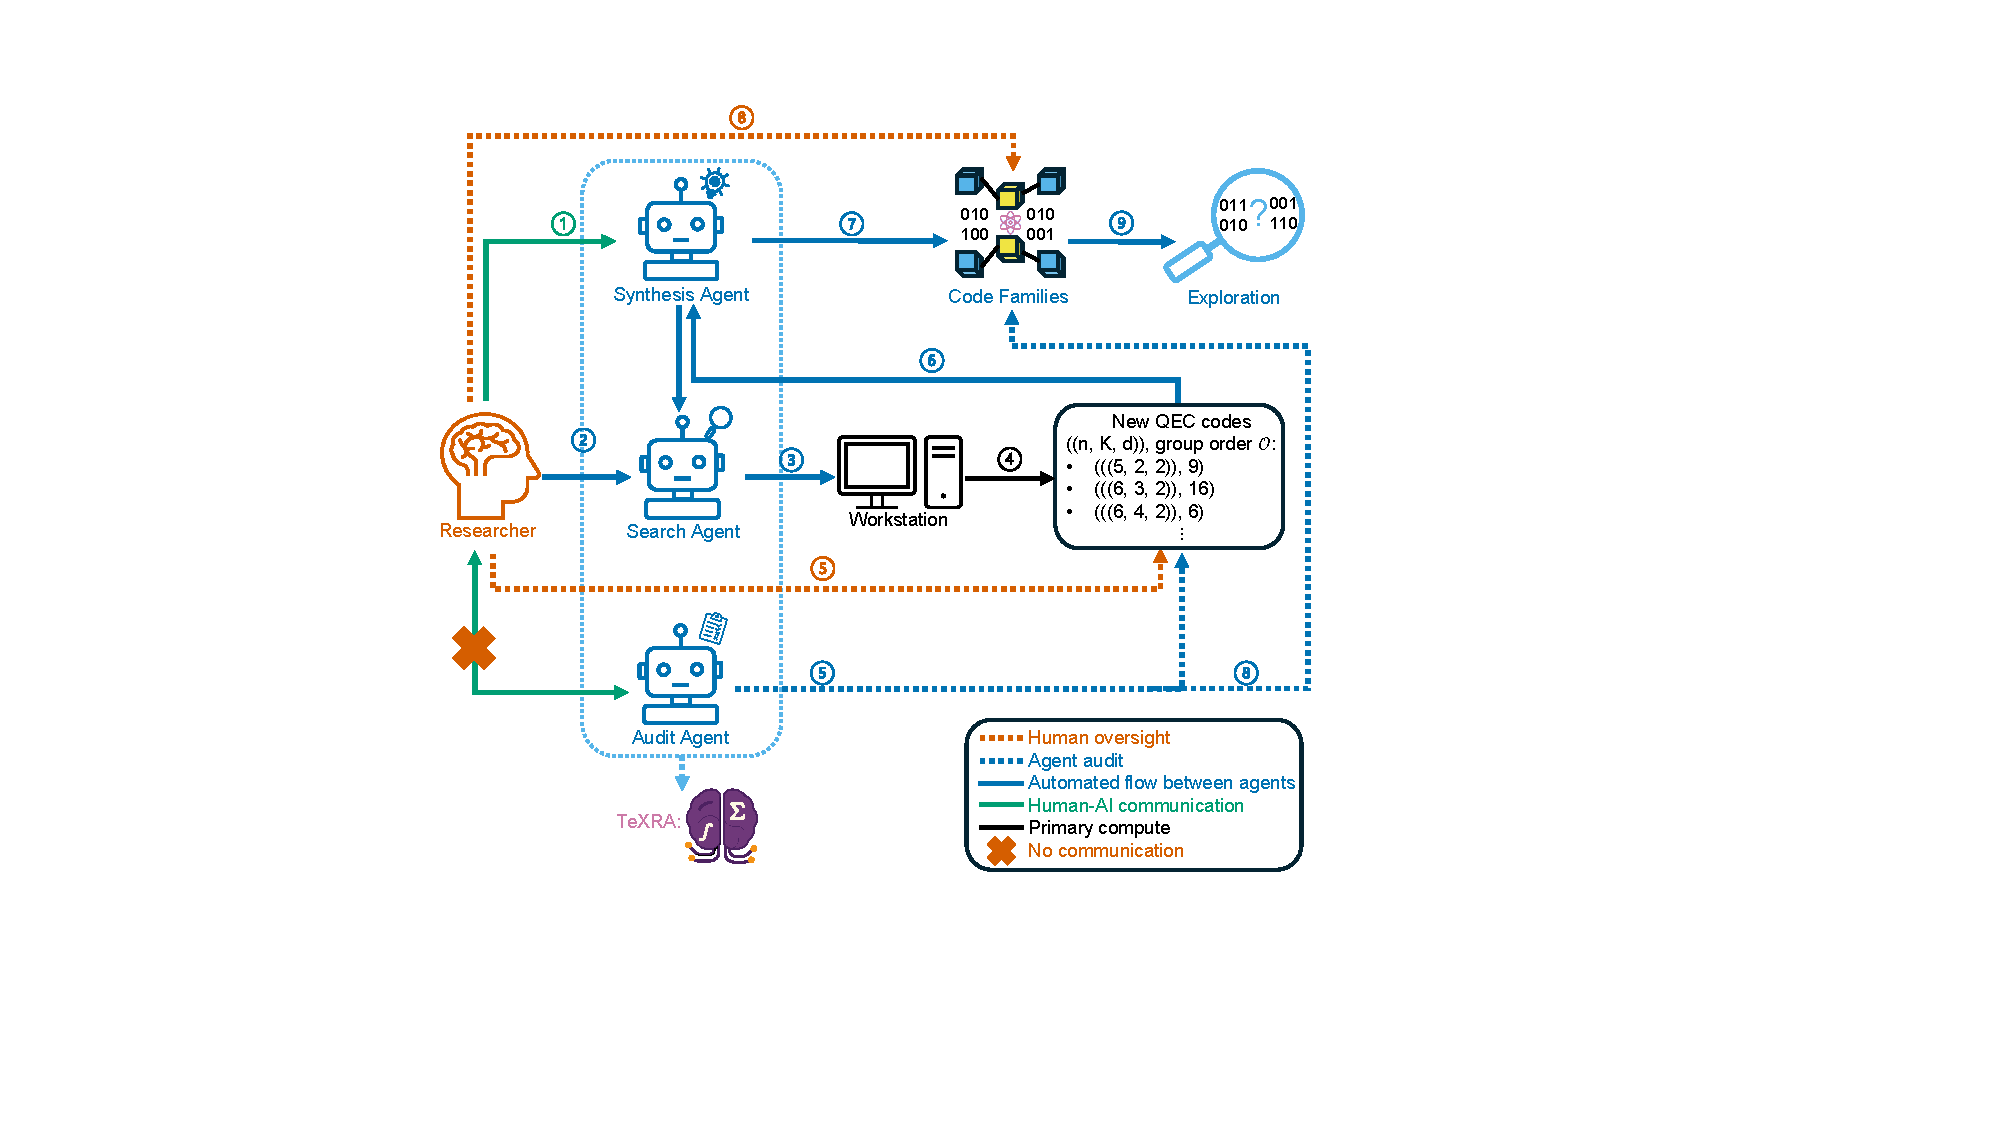
\includegraphics[width=0.9\linewidth]{Fig.1.pdf}
    \caption{Multi-agent human--AI co-design system for quantum code discovery. 
    The researcher seeds the Synthesis Agent with basic definitions and a worked example (step 1), reviews the outputs (step 5), and decides when to promote candidates to code families (step 8). The Synthesis Agent deduces a combinatorial reformulation of the problem and proposes parameter templates (step 2). Guided by these proposals, the Search Agent generates and executes search code on a local workstation (step 3) to enumerate candidate quantum error-correcting codes with specified parameters $((n,K,d))$ and diagonal-transversal group order~$\mathcal O$ (step 4). The resulting candidates are passed to the Audit Agent, which, along with the researcher, independently verifies that they satisfy the exact KL and transversal conditions (step 5). Verified results are fed back to the Synthesis Agent to abstract general code families (step 7) and construct extended examples (Step 9). Legend: Blue arrows denote automated communication between agents; green arrows indicate human--AI interaction; orange arrows represent human oversight; black arrows mark primary compute; and the red cross highlights a deliberate no-communication barrier that preserves the independence of the audit process.}
    \label{fig1:sche}
\end{figure}

Quantum error correction encodes information into a $K$-dimensional subspace of an $n$-qubit system, enabling detection or correction of errors~\cite{Nielsen2010Quantum,Calderbank1998Quantum,Steane1996Error,Knill1997Theory}. Logical operations must avoid spreading errors; transversal gates, which act independently on each physical qubit, address this but are constrained by no-go theorems that forbid universally transversal gate sets~\cite{Zeng2011Transversality,Eastin2009Restrictions} and impose stringent group-theoretic constraints~\cite{Liu2023Approximate,Anderson2016Classification}. Beyond stabilizer codes~\cite{Calderbank1998Quantum,Gottesman1997Stabilizer}, nonadditive constructions~\cite{Rains1997Nonadditive} expand the design space, including codeword-stabilized (CWS) codes~\cite{Cross2009Codeword,Chuang2009Codeword,Yu2007Graphical,Yu2008Nonadditive,Grassl2008Nonadditive}, permutation-invariant (PI) codes~\cite{Pollatsek2004Permutationally,Ouyang2014Permutation,Ouyang2021Permutation,Ouyang2024Measurement}, and broader nonadditive families~\cite{Du2024Characterizing}. Small stabilizer subsystem codes have recently been systematically enumerated~\cite{Cross2025Small}. Their transversal structure is rich, from classical nonadditive phenomena~\cite{Rains2002Quantum} to recent permutation-invariant codes realizing the binary icosahedral group $2\mathrm{I}$~\cite{Kubischta2023Family} and higher-order diagonal phases~\cite{Kubischta2024Permutation}. The Subset-Sum Linear Programming (SSLP) framework~\cite{Zhang2025Transversal} reframes the \emph{diagonal-transversal} problem as congruence structure plus linear $Z$-marginals, revealing a richer landscape of nonadditive codes and motivating the question: for given $((n,K,d))$ with distance $d$, which transversal groups can arise and how can the corresponding codes be constructed?

We address this question for diagonal transversal gates, which yield abelian (typically cyclic) logical groups, using the SSLP framework~\cite{Zhang2025Transversal}. SSLP partitions computational basis strings into groups using modular arithmetic: each logical basis state is assigned to one group, so a transversal diagonal gate---applying phases independently to each qubit---induces a predictable logical phase determined by the group label. The Knill--Laflamme (KL) conditions~\cite{Knill1997Theory} then decompose into (i) structural requirements on group separation preventing bit-flip errors from creating unwanted interference between logical states, and (ii) constraints on how quantum amplitudes distribute within groups so that single-qubit measurement statistics match across logical states. The latter are linear in the squared amplitudes (probabilities). This structure---discrete choices (which groups?) plus linear feasibility (which probability distributions?)---makes systematic search tractable while still requiring both combinatorial enumeration and analytical pattern recognition.

Our workflow begins with the researcher providing initial definitions and a worked example in LaTeX, establishing notation and error-correction requirements. The Synthesis Agent proposes combinatorial formulations and parameter families, the Search Agent realizes these as executable Python code and performs large-scale enumeration on the local workstation, and the Audit Agent independently verifies candidates using separate implementations to confirm that KL conditions and the transversality are correct. Verified codes feed back to the Synthesis Agent, which identifies structural patterns and derives closed-form families, while humans guide search strategies and validate agent-proposed generalizations.

We focus initially on distance-$d=2$ codes with nondegenerate residues (each logical state occupies a distinct modular class), where SSLP's structure enables systematic exploration. Across this search regime, the workflow yields a certified catalogue of 14,116 previously unreported codes. For code dimensions $K{\in}\{2,3,4\}$ on up to $n=6$ physical qubits, the Search Agent discovers new codes realizing cyclic gate orders ranging from 2 to 18, with explicit constructions specifying exact parameters, probability amplitudes, and phases (Sec.~\ref{subsec:catalogue}). The Synthesis Agent extracts analytical understanding, proposing closed-form infinite families that recover and generalize many of these instances (Sec.~\ref{subsec:families}). Relaxing the nondegenerate-residue assumption, the agents construct a $((6,4,2))$ code realizing a controlled-phase gate $\mathrm{diag}(1,1,1,i)$ where three logical states share a residue class (Sec.~\ref{subsec:extension}). This illustrates how the multi-agent approach scales from tractable regimes enabling classification to more complex settings where agents complement human insight.

\section{Results}
\label{sec:results}

\subsection{Problem formulation}
\label{subsec:formulation}

Our goal is to identify small-distance quantum codes that admit high-order diagonal transversal logical actions, and to characterize the landscape of such solutions discovered by our multi-agent search.
Concretely, we focus on distance-2 codes on $n$ physical qubits that encode a $K$-dimensional logical subspace and support a transversal diagonal operator whose induced logical phases form a cyclic group of order $\mathcal{O}$.
The Results section will (i) summarize the representative codes found across $K$ (Table~\ref{tab:search_codes}), (ii) quantify the attainable transversal orders and structural regularities, and (iii) validate candidates by explicitly solving the Knill--Laflamme (KL) conditions beyond the diagonal constraints. In total, our systematic sweeps in this regime produce 14,116 certified solutions, from which we report representative codes and aggregate statistics below. All technical details of optimization and verification are deferred to Methods and Supplementary Notes; here we only introduce the minimal objects needed to interpret the reported tables and figures.

\textbf{Distance-2 error-detection constraints.}
A quantum code is a $K$-dimensional subspace spanned by orthonormal logical states $\{\ket{j_L}\}_{j=0}^{K-1}$.
For distance $d=2$, we require detectability of all single-qubit Pauli errors.
Operationally, this means that each single-qubit Pauli $P_i\in\{X_i,Y_i,Z_i\}$ cannot reveal logical information: its expectation value must be identical across all logical basis states, and it cannot create coherence between distinct logical states.
The $Z$-type constraints depend only on the computational-basis probability mass of each $\ket{j_L}$, whereas the $X/Y$ constraints additionally couple amplitudes of Hamming-1 neighbors, which is the main source of nonconvexity in direct searches.

\textbf{Diagonal transversal structure via subset-sum partitioning.}
To target diagonal transversal gates, we specify a modulus $m$ and a weight vector $\mathbf w\in(\mathbb{Z}_m)^n$.
They define a modular ``subset-sum'' map $x\mapsto \langle \mathbf w,x\rangle\!\!\pmod m$ over bitstrings $x\in\{0,1\}^n$, which partitions the computational basis into residue classes.
We enforce that each logical state is supported on one residue class, indexed by residues $\mathbf S=(S_0,\dots,S_{K-1})$ (with $S_0=0$ by convention).
This simple structural constraint is what makes large-scale search feasible: when the selected residues are distinct, the logical supports are disjoint, guaranteeing orthogonality by construction and allowing us to reason about diagonal logical actions without committing to explicit amplitudes at the outset.

Under this setup, the transversal diagonal operator $U(\mathbf w,m)=\bigotimes_{i=1}^n Z\!\left(\tfrac{2\pi w_i}{m}\right)$
acts on basis states by a residue-dependent phase.
As a consequence, it acts diagonally on the logical basis with eigenphases determined solely by $\{S_j\}$, and the induced logical cyclic group has projective order
$\mathcal{O}=m/\gcd(m,S_1,\dots,S_{K-1})$.
In the Results, we therefore report $(n,K)$ together with $(m,\mathbf w,\mathbf S)$-dependent quantities such as $\mathcal{O}$ as primary descriptors of each discovered code.

\textbf{SSLP~\cite{Zhang2025Transversal}}.
The subset-sum linear program (SSLP) provides an efficient feasibility filter using only the $Z$-type KL constraints: it searches for per-logical-state probability distributions supported on the chosen residue classes whose single-site $Z$ marginals match across all logical states.
Passing this filter is necessary but not sufficient; it identifies promising $(m,\mathbf w,\mathbf S)$ candidates that we then refine by solving the remaining $X/Y$-type KL constraints via numerical optimization.
This division of labor: (i) combinatorial support selection, (ii) linear feasibility screening, and (iii) full KL verification is the lens through which we present and interpret the empirical discoveries throughout the Results.

\subsection{Catalogue of distance-2 diagonal-transversal code ($K \leq 4$, $n \leq 6$)}
\label{subsec:catalogue}

We next characterise the landscape of distance-2 diagonal-transversal codes uncovered by the multi-agent SSLP search in the regime $K\leq 4$ and $n\leq 6$. After solving all subset-sum instances, performing rational reconstruction, and re-checking the Knill–Laflamme and logical transversality conditions, we obtain a certified catalogue of nondegenerate codes. In total, the certified catalogue contains 14,116 distinct codes. Table~\ref{tab:search_codes} lists human-readable representatives, while Fig.~\ref{fig:search_codes} summarises global statistics over the full search space.

\begin{table*}[t]
\centering
\footnotesize
\setlength{\tabcolsep}{3.2pt}
\renewcommand{\arraystretch}{0.92}

\caption{Representative distance-2 diagonal-transversal codes discovered by the multi-agent search. Rows are grouped by code dimension $K$. Each entry lists the transversal order $\mathcal O$, modulus $m$, length $n$, sorted weight vector $\mathbf w$, and residue set $\mathbf{S}=\tup{0,S_{1},\ldots,S_{K-1}}$.}
\label{tab:search_codes}

% =========================
% Panel A: K=2 (two-up)
% =========================
\textbf{Panel A: $K=2$}\par\vspace{2pt}
\begin{tabular*}{\textwidth}{@{\extracolsep{\fill}} R R R L L : R R R L L @{}}
\toprule
\multicolumn{1}{c}{$\mathcal O$} &
\multicolumn{1}{c}{$m$} &
\multicolumn{1}{c}{$n$} &
\multicolumn{1}{c}{$\mathbf w$} &
\multicolumn{1}{c}{$\mathbf S$} &
\multicolumn{1}{c}{$\mathcal O$} &
\multicolumn{1}{c}{$m$} &
\multicolumn{1}{c}{$n$} &
\multicolumn{1}{c}{$\mathbf w$} &
\multicolumn{1}{c}{$\mathbf S$} \\
\midrule
2   & 4   & 4 & \tup{1,1,1,1}              & \tup{0,2}  &
2   & 4   & 5 & \tup{1,1,1,1,1}            & \tup{0,2}  \\
3   & 6   & 5 & \tup{1,1,1,1,3}            & \tup{0,4}  &
4   & 8   & 5 & \tup{1,1,1,3,3}            & \tup{0,6}  \\
5   & 5   & 5 & \tup{1,1,1,1,1}            & \tup{0,2}  &
6   & 6   & 5 & \tup{2,2,2,3,3}            & \tup{0,1}  \\
7   & 7   & 5 & \tup{1,1,1,2,2}            & \tup{0,3}  &
8   & 8   & 5 & \tup{1,1,2,2,4}            & \tup{0,5}  \\
9   & 9   & 5 & \tup{1,1,2,2,3}            & \tup{0,4}  &
2   & 4   & 6 & \tup{1,1,1,1,1,1}          & \tup{0,2}  \\
3   & 6   & 6 & \tup{1,1,1,1,1,1}          & \tup{0,2}  &
5   & 5   & 6 & \tup{1,1,1,1,1,1}          & \tup{0,2}  \\
6   & 6   & 6 & \tup{2,2,2,2,3,3}          & \tup{0,1}  &
7   & 7   & 6 & \tup{1,1,1,1,1,2}          & \tup{0,3}  \\
8   & 8   & 6 & \tup{1,1,1,1,1,4}          & \tup{0,5}  &
9   & 9   & 6 & \tup{1,1,1,1,2,3}          & \tup{0,4}  \\
10  & 10  & 6 & \tup{1,1,1,1,4,6}          & \tup{0,7}  &
11  & 11  & 6 & \tup{1,1,1,1,4,4}          & \tup{0,8}  \\
12  & 12  & 6 & \tup{1,1,1,2,3,4}          & \tup{0,5}  &
13  & 13  & 6 & \tup{1,1,1,2,5,5}          & \tup{0,10} \\
14  & 14  & 6 & \tup{1,1,1,3,3,6}          & \tup{0,9}  &
15  & 15  & 6 & \tup{1,1,2,2,5,6}          & \tup{0,11} \\
16  & 16  & 6 & \tup{1,1,2,3,4,5}          & \tup{0,7}  &
17  & 17  & 6 & \tup{1,1,2,4,4,6}          & \tup{0,8}  \\
18  & 18  & 6 & \tup{1,2,3,4,5,6}          & \tup{0,11} &
{}  & {}  & {}& {}                         & {}         \\
\bottomrule
\end{tabular*}

\vspace{0.9em}

% =========================
% Panel B: K=3 (two-up)
% =========================
\textbf{Panel B: $K=3$}\par\vspace{2pt}
\begin{tabular*}{\textwidth}{@{\extracolsep{\fill}} R R R L L : R R R L L @{}}
\toprule
\multicolumn{1}{c}{$\mathcal O$} &
\multicolumn{1}{c}{$m$} &
\multicolumn{1}{c}{$n$} &
\multicolumn{1}{c}{$\mathbf w$} &
\multicolumn{1}{c}{$\mathbf S$} &
\multicolumn{1}{c}{$\mathcal O$} &
\multicolumn{1}{c}{$m$} &
\multicolumn{1}{c}{$n$} &
\multicolumn{1}{c}{$\mathbf w$} &
\multicolumn{1}{c}{$\mathbf S$} \\
\midrule
3   & 6   & 6 & \tup{1,1,1,1,3,3}          & \tup{0,2,4}   &
4   & 8   & 6 & \tup{1,1,1,3,3,3}          & \tup{0,2,4}   \\
6   & 12  & 6 & \tup{1,1,1,5,5,7}          & \tup{0,6,10}  &
8   & 16  & 6 & \tup{1,1,4,4,7,7}          & \tup{0,2,8}   \\
10  & 10  & 6 & \tup{1,1,1,4,4,4}          & \tup{0,2,5}   &
12  & 12  & 6 & \tup{2,2,3,3,4,4}          & \tup{0,6,7}   \\
14  & 14  & 6 & \tup{1,1,3,4,6,6}          & \tup{0,2,7}   &
15  & 15  & 6 & \tup{1,1,4,4,6,9}          & \tup{0,2,10}  \\
16  & 16  & 6 & \tup{1,2,4,4,6,7}          & \tup{0,8,11}  &
{}  & {}  & {}& {}                         & {}            \\
\bottomrule
\end{tabular*}

\vspace{0.9em}

% =========================
% Panel C: K=4 (two-up)
% =========================
\textbf{Panel C: $K=4$}\par\vspace{2pt}
\begin{tabular*}{\textwidth}{@{\extracolsep{\fill}} R R R L L : R R R L L @{}}
\toprule
\multicolumn{1}{c}{$\mathcal O$} &
\multicolumn{1}{c}{$m$} &
\multicolumn{1}{c}{$n$} &
\multicolumn{1}{c}{$\mathbf w$} &
\multicolumn{1}{c}{$\mathbf S$} &
\multicolumn{1}{c}{$\mathcal O$} &
\multicolumn{1}{c}{$m$} &
\multicolumn{1}{c}{$n$} &
\multicolumn{1}{c}{$\mathbf w$} &
\multicolumn{1}{c}{$\mathbf S$} \\
\midrule
4   & 8   & 6 & \tup{1,1,1,3,3,3}          & \tup{0,2,4,6}  &
6   & 12  & 6 & \tup{1,1,3,3,5,5}          & \tup{0,2,6,10} \\
\bottomrule
\end{tabular*}

\end{table*}

\begin{figure}[t]
    \centering
    \begin{minipage}[t]{0.67\linewidth}
        \centering
        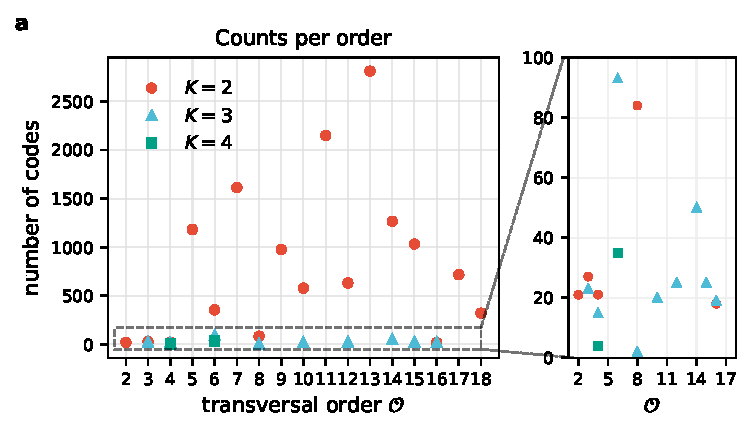
\includegraphics[width=\linewidth]{Fig.3a.pdf}\par\vspace{3pt}
        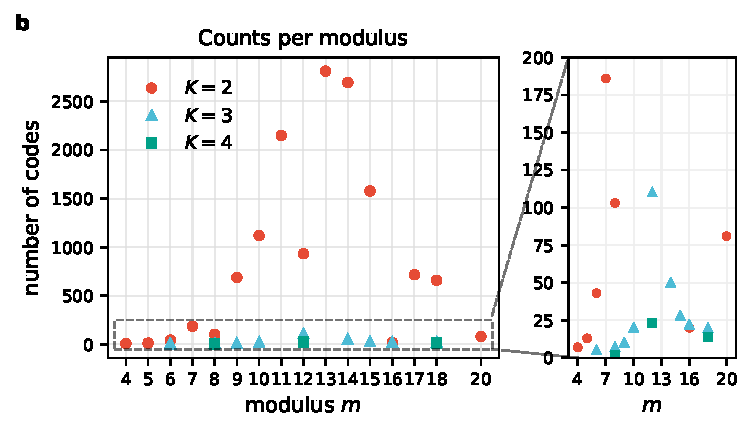
\includegraphics[width=\linewidth]{Fig.3b.pdf}
    \end{minipage}\hfill
    \raisebox{-0.4\linewidth}{%
    \begin{minipage}[t]{0.33\linewidth}
        \centering
        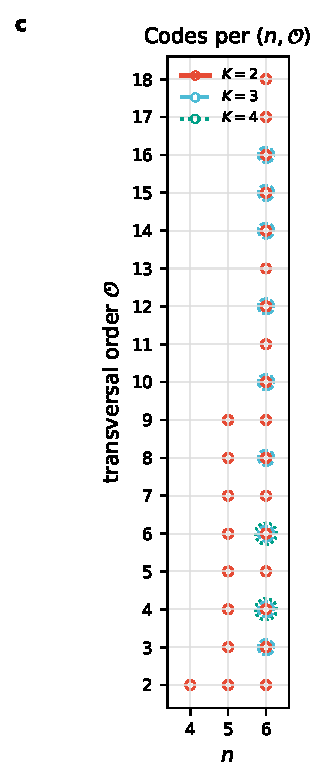
\includegraphics[width=\linewidth]{Fig.3c.pdf}
    \end{minipage}}
    \caption{Global statistics of the diagonal-transversal code catalogue. We aggregate all nondegenerate distance-$2$ codes with $K\leq 4$ and $n\leq 6$ obtained from the multi-agent SSLP search and catalogued in Table~\ref{tab:search_codes}. (a) Number of codes found at each transversal order $\mathcal{O}$, shown on a logarithmic scale and separated by logical dimension $K=2,3,4$ (colours and markers as indicated in the legend). (b) Number of codes as a function of the modulus $m$, again on a logarithmic scale and resolved by $K$. (c) Existence landscape in the $(n,\mathcal{O})$ plane: for each pair $(n,\mathcal{O})$ where at least one code is found, we draw concentric rings centred at $(\mathcal{O},n)$, with the inner, middle and outer rings indicating the presence of codes with $K=2$, $K=3$ and $K=4$, respectively. Panels~(a) and~(b) encode absolute counts, while panel~(c) highlights which regions of the $(n,\mathcal{O})$ grid are populated by different logical dimensions.}
    \label{fig:search_codes}
\end{figure}


Each row of Table~\ref{tab:search_codes} specifies a canonical code for a distinct triple $(K,n,\mathcal{O})$, given by its modulus $m$, sorted weight vector $\mathbf{w}$ and residue set $\mathbf{S}=(0,S_1,\dots,S_{K-1})$. For $K=2$ the landscape is unexpectedly dense: all orders $\mathcal{O}=2,\dots,18$ appear at $n=6$, and several low orders admit shorter realisations at $n=4$ or $5$. Many examples use nearly homogeneous weights such as $(1,1,1,1,1,1)$ or permutations of $\{1,2,3,4,5,6\}$, whereas larger orders tend to require more heterogeneous patterns. The corresponding residue sets exhibit simple arithmetic structure, typically involving small integers or approximately symmetric placements in $\mathbb{Z}_m$, reflecting the balanced subset-sum partitions enforced by the SSLP ansatz. For $K=3$ and $K=4$ the catalogue is sparser but still spans a broad range of orders; all currently known examples sit at $n=6$, demonstrating that higher logical dimensions can be achieved with very compact blocklength once the optimisation is pushed to high numerical accuracy.

Figure~\ref{fig:search_codes}a aggregates all nondegenerate codes by transversal order. On the logarithmic vertical scale, orders $\mathcal{O}\leq 5$ for $K=2$ dominate the statistics, while the count decays gradually towards $\mathcal{O}=18$. Several intermediate orders, such as $\mathcal{O}=4$ and $10$, support noticeably more codes than their neighbours, indicating particularly favourable congruence structure in the underlying subset-sum constraints. The curves for $K=3$ and $K=4$ are shifted down by several orders of magnitude, consistent with the reduced combinatorial volume for higher-dimensional logical spaces at fixed $(n,m)$ and with the additional convex-hull intersection constraint. Nevertheless, most admissible orders host at least one $K=3$ code, and a subset also supports a $K=4$ code, showing that diagonal-transversal resources are not confined to very low logical order.

Figure~\ref{fig:search_codes}b reorganises the same data as a function of the modulus. Certain moduli support markedly richer families of codes, with $m\approx 10$–$18$ particularly prolific for $K=2$. Only a subset of these moduli admit higher-$K$ codes, but overlap is common: several values of $m$ carry simultaneous solutions for $K=2$ and $K=3$, and some of these also host $K=4$ codes. This arithmetic clustering suggests that once a modulus supports one feasible residue pattern, nearby patterns often generate additional solutions at different orders and with different weight profiles, turning each “good” modulus into a local family of diagonal-transversal constructions.

The existence landscape in the $(n,\mathcal{O})$ plane is disentangled from absolute counts in Fig.~\ref{fig:search_codes}c. For each pair where at least one code is found we place concentric rings, with the inner, middle and outer circles indicating the presence of $K=2$, $K=3$ and $K=4$ codes, respectively. The inner ring almost saturates the accessible grid for $n=6$, consistent with the dense $K=2$ statistics in panels~(a) and~(b), while $K=3$ and $K=4$ appear exclusively at $n=6$ but over many orders. Notably, we do not observe any point where a $K=3$ or $K=4$ code exists without a companion $K=2$ code at the same $(n,\mathcal{O})$, indicating that the $K=2$ solutions often form a combinatorial backbone from which higher-dimensional constructions can be obtained.

Taken together, Table~\ref{tab:search_codes} and Fig.~\ref{fig:search_codes} provide a compact catalogue of small-distance diagonal-transversal codes (see Table~\ref{tab:group_ranges_by_n} for the corresponding numerical $\lambda^*$ ranges). Beyond furnishing explicit rational certificates, the statistics highlight where the landscape is dense, which orders and moduli are especially productive, and where gaps remain open. These observations guide our extensions to larger $n$ and higher distances, and suggest concrete analytical questions about when a given diagonal-transversal group can be realised by a nonadditive code.

\subsection{Analytical families and scaling patterns}
\label{subsec:families}

The catalogue of certified codes obtained by the multi-agent search serves as a dataset from which to extract structure. After completing sweeps over $n\le 6$ and $K\in\{2,3,4\}$, the Synthesis Agent analysed audited instances selected by the human researcher and proposed parameterizations that explain recurring residue patterns, amplitude assignments, and logical phase structures. From these proposals we identified several infinite families of distance-2 codes that can be constructed analytically within the SSLP framework (Methods, Sec.~\ref{subsec:families-methods}). We highlight two representative families that capture the main scaling patterns.

\subsubsection{Family I: $C_0=\{0^n,1^n\}$}
\label{subsubsec:family1}

The first family is seeded by the extremal codewords $\{0^n,1^n\}$. For each $n\ge2$ we choose a modulus $m\ge n$ and weight vector
$\mathbf w=(1,\dots,1,m-(n-1))\in(\mathbb Z_m)^n$ so that the subset-sum class with residue~$0$ contains exactly
$C_0=\{0^n,1^n\}$. For any residue $s$ in an allowed range (determined by the subset-sum structure), the class $C_s$ splits into two Hamming-weight slices: strings of weight $s$ with a $0$ on the last qubit, and strings of weight $t=n-1+s-m$ with a $1$ on the last qubit. Within the SSLP formulation there is a site-symmetric probability assignment on $C_0$ and $C_s$ that equalizes all single-qubit $Z$-marginals and hence solves the convex part of the KL conditions.

This construction yields a pair of logical states supported on $C_0$ and $C_s$ with closed-form amplitudes and common expectation value $\langle Z_i\rangle=1-\tfrac{2s}{m}$ at every site. The associated diagonal transversal gate
$U(\mathbf w,m)=\bigotimes_j Z(2\pi w_j/m)$ acts on the code space as
$\overline U=\mathrm{diag}(1,\omega_m^{s})$, so the generated logical group has order
\[
  \mathcal O=\frac{m}{\gcd(m,s)} .
\]
Whenever $s$ avoids a small set of forbidden residues, the residue-shift screening rule inherited from the search guarantees that all single-qubit $X/Y$ off-diagonal KL terms vanish combinatorially, so the code has distance~2 (see Methods: Section~\ref{subsubsec:proof_family_1} for a proof).

This family explains many of the high-order entries in the catalogue. For example, at $((n,K))=((5,2))$ taking $m=5$ and $s=2$ reproduces a $((5,2,2))$ code with $\overline U=\mathrm{diag}(1,\omega_5^2)$, while at $((n,K))=((6,2))$ taking $m=7$ and $s=3$ produces a $((6,2,2))$ code with $\overline U=\mathrm{diag}(1,\omega_7^3)$ and order~$\mathcal O=7$, matching the independently discovered instances.


\subsubsection{Family II: even-parity subset-sum codes}
\label{subsubsec:family2}

A second family arises by restricting supports to the even-parity subcode
$\mathsf E=\{\sigma\in\{0,1\}^n:\mathrm{wt}(\sigma)\equiv 0\ (\bmod\ 2)\}$ for even $n$. Given a modulus $m$, a weight vector $\mathbf w\in(\mathbb Z_m)^n$, and distinct residues $\mathbf S=\{S_0,\dots,S_{K-1}\}\subset\mathbb Z_m$ with $S_0=0$, we consider the even-parity subset-sum classes
\[
  C^{(+)}_{S_k}(\mathbf w)=\bigl\{\sigma\in\mathsf E:\textstyle\sum_{j=1}^{n} w_j\sigma_j\equiv S_k \pmod m\bigr\}
\]
and define logical states as uniform superpositions over these supports:
\[
    \ket{k_L} = \frac{1}{\sqrt{|C^{(+)}_{S_k}|}}\sum_{\sigma\in C^{(+)}_{S_k}}\ket{\sigma},\qquad k=0,\dots,K-1.
\]
The diagonal transversal gate $U(\mathbf w,m)$ induces $\overline U=\mathrm{diag}(\omega_m^{S_0},\dots,\omega_m^{S_{K-1}})$, so the logical group generated by $U$ has order $\mathcal O = m / \gcd(m,S_1,\dots,S_{K-1})$.

The distance-2 property is enforced in two complementary ways. Because all supports lie in the even-parity subcode, any single-qubit $X_i$ or $Y_i$ error maps basis states to odd-parity strings outside the support of every logical state, so all $X/Y$ matrix elements vanish automatically. For $Z$-error constraints we require each support $C^{(+)}_{S_k}$ to be \emph{column-balanced}: for every qubit index $i$, exactly half of the strings in $C^{(+)}_{S_k}$ have a '$1$' at position~$i$. This yields $\langle k_L|Z_i|k_L\rangle=0$ for all logical labels $k$, while disjoint supports ensure $\langle k_L|Z_i|\ell_L\rangle=0$ for $k\neq\ell$. Sufficient symmetry conditions on $\mathbf w$ and $\mathbf S$ that enforce column balance, together with concrete constructions, are given in the Methods (Section~\ref{subsubsec:proof_family_2}) and Supplementary Information (Section~\ref{subsubsec:supp:family2}).

Within this family we obtain examples with different dimensions and logical orders. Choosing suitable $(m,\mathbf w,\mathbf S)$ for $n=4$ and $n=6$ yields $((n,K,d))=((4,2,2))$ and $((6,2,2))$ codes with logical order $\mathcal O=2$, while a construction at $n=6$ with $K=3$ realizes
$\overline U=\mathrm{diag}(1,\omega_9^3,\omega_9^6)$ of order $\mathcal O=3$. These families account for a substantial fraction of the catalogue entries with small $n$ and show how multi-agent-guided analysis can lift isolated search hits into scalable code constructions.


\subsection{Beyond nondegenerate residues}
\label{subsec:extension}

All constructions discussed so far impose two simplifying guards on the SSLP framework: 
(i) \emph{residue nondegeneracy}, where each logical state $\ket{j_L}$ is supported on a distinct residue class $C_{S_j}(\mathbf w)$, and 
(ii) a strict classical union distance $d(C)=2$. 
Together these reduce the design problem to combinatorial residue screens plus small $Z$-only programs: all single-qubit $X/Y$ matrix elements vanish by residue bookkeeping, while the remaining $Z$-marginal equalities become linear feasibility tests. The catalogue in the previous sections was obtained entirely within this nondegenerate regime.

To access a richer design space, we now relax these guards. 
If several logical states share the same residue class, the diagonal transversal $U(\mathbf w,m)$ induces a degenerate logical action on that block, and the Knill--Laflamme conditions must be enforced by structured amplitude patterns that cancel $X/Y/Z$ matrix elements. 
Dropping the requirement $d(C)=2$ likewise allows Hamming-1 neighbours inside the union support, further shifting the burden from combinatorial separation to amplitude design. 
Although search in this regime is more demanding, the multi-agent system can still discover concrete examples when given a targeted specification.

As a test case, we ask the agents to construct a distance-2 code implementing a non-trivial two-qubit logical gate, namely a controlled phase with eigenvalues $(1,1,1,i)$. 
The Synthesis and Search Agents jointly identify a residue-degenerate $((6,4,2))$ code with modulus $m=4$ and weight vector $\mathbf w=(1,3,2,2,2,2)\in\mathbb Z_4^6$, for which the residue of $x=(x_1,\dots,x_6)$ is
\[
  \operatorname{res}(x)\equiv \mathbf w\cdot x \pmod 4
  = x_1 - x_2 + 2\,\bigl(x_3\oplus x_4\oplus x_5\oplus x_6\bigr)\pmod 4,
\]
determined by the first two bits and the parity of the last four. 
The code exploits this structure by organizing the last four qubits into even- and odd-parity subsets and placing three logical states in residue value $0$, reserving residue value $1$ for the fourth.

Concretely, three logical states $(\ket{0_L},\ket{1_L},\ket{2_L})$ are supported on even-parity strings in the last four qubits with $(x_1,x_2)=(00)$ or $(11)$ and differ only by $\{\pm1\}$ sign patterns given by characters on $\mathbb F_2^3$, which guarantee orthogonality within the residue-$0$ block and the required $Z$-marginal equalities. 
The fourth state $\ket{3_L}$ lives on residue-$1$ strings that mix $(10)$ and $(01)$ on the first two qubits with even and odd tail parity, chosen so that all single-qubit $X/Y$ matrix elements between $\ket{3_L}$ and the residue-$0$ block vanish by residue and parity arguments. 
All four logical states have flat amplitudes in modulus, so the construction is fully determined by supports and sign characters.

A direct verification (Methods, Sec.~\ref{subsec:families-methods}, and Supplementary Note~\ref{supp:degenerate-642}) confirms that every weight-1 Pauli operator $E\in\{X_i,Y_i,Z_i\}$ satisfies the distance-2 Knill--Laflamme equations
$\bra{j_L}E\ket{k_L}=0$ for $j\neq k$ and equal diagonals across $j$. 
The diagonal transversal $U=\bigotimes_{j=1}^6 Z\!\left(\tfrac{\pi}{2} w_j\right)$
acts on a basis state $\ket{x}$ as $U\ket{x}=i^{\operatorname{res}(x)}\ket{x}$ and therefore induces $U_L=\mathrm{diag}(1,1,1,i)$ on the logical basis $\{\ket{0_L},\ket{1_L},\ket{2_L},\ket{3_L}\}$. 
This $((6,4,2))$ controlled-phase example lies strictly beyond the nondegenerate-residue screen used in our systematic sweeps (three logical states share residue value $0$), showing that relaxing the simplifying guards can yield genuinely new codes and logical gates within the SSLP framework. 

\section{Discussion and Outlook}
\label{sec:discuss}

We have developed an automated discovery pipeline that finds quantum error-correcting codes with prescribed transversal gates, producing a certificate-backed catalog of distance-2 codes on small qubit numbers. With 14,116 new codes found in the $K\in{2,3,4}$, $n\le 6$ regime, our results show that agentic orchestration can support catalogue-level discovery with independent verification. The workflow runs on TeXRA~\cite{Texra2025TeXRA} with GPT-5~\cite{Openai2025GPT} and uses three coordinated agents to explore parameter spaces, convert numerical solutions to exact rational forms, and verify results independently. For $K \in \{2,3,4\}$ on $n \le 6$ qubits we obtain a collection of \emph{new} codes with cyclic transversal gate orders from 2 to 18, each certified with exact Knill--Laflamme equations~\cite{Knill1997Theory}, and extend these instances into infinite analytical families.

Designing the multi-agent architecture was driven by practical limitations of frontier models. Finite context windows~\cite{Openai2025GPT,Anthropic2024Model} can accumulate small errors that propagate through long chains of reasoning, and models often exhibit anchoring behavior, defending earlier conclusions instead of revising them~\cite{Lightman2023Lets}. We therefore separated search and verification: a Search Agent proposes constructions, while an independent Audit Agent without access to the search transcripts generates its own code to check numerical instances and validates the derivations of the closed-form families, mirroring the software engineering principle of independent testing~\cite{Jimenez2024SWEbench}. Additional agents handle notation checking and redundancy removal to mitigate drift across sessions.

Human oversight remained essential: resetting conversations prevented context pollution, concrete examples grounded abstract claims, and humans edited manuscripts for coherence and notation. All new mathematical results---discovered codes, analytical families, closed-form proofs---were generated by agents, while humans validated correctness, guided strategies, and shaped presentation. This division of labor appears effective whenever problems have the right structure.

The key technical step, identified together with the agents, was to use the SSLP framework~\cite{Zhang2025Transversal} with the \emph{classical union distance} condition $d(C)=2$ to reduce distance-2 feasibility to tractable subproblems. Modular residue classes partition computational basis strings so that transversal diagonal gates induce predictable logical phases; when each logical state occupies a distinct residue class, single-qubit $X$ and $Y$ errors automatically satisfy off-diagonal KL constraints by disjoint support, and the remaining $Z$-marginal conditions become linear equations on probability amplitudes. This turns a nonlinear, high-dimensional feasibility problem into discrete screening plus convex optimization, enabling systematic enumeration and exact analytical reconstruction via continued-fraction approximation~\cite{Ferguson1999Analysis,Lenstra1982Factoring} and integer-preserving projection~\cite{Schrijver1986Theory}.

Although our application focuses on distance-2 codes with diagonal transversals, the methodology suggests a broader paradigm for AI-assisted discovery in theoretical physics and mathematics. It combines (1) mathematical reformulation that exposes tractable substructure; (2) multi-agent orchestration~\cite{Wu2023AutoGen,Du2023Improving} with specialized roles; and (3) problems whose solutions are hard to generate but easy to check~\cite{Glazer2024FrontierMath,Lu2025Can}. Similar structural conditions arise in classification problems across mathematical physics, such as symmetry-protected phases~\cite{Chen2013Symmetry,Zeng2019Quantum}. In our implementation, the Synthesis Agent uses derivation-then-edit workflows~\cite{Wei2022Chainofthought,Shinn2023Reflexion} to derive combinatorial reformulations and screening rules, the Search Agent employs tool-use loops~\cite{Yao2023ReAct,Schick2023Toolformer} to generate and run code at scale, and the Audit Agent operates behind a no-communication barrier in the spirit of independent testing~\cite{Jimenez2024SWEbench}. 

For quantum error correction, our catalog enlarges the known nonadditive design space~\cite{Rains1997Nonadditive,Rains2002Quantum} beyond prior constructions~\cite{Cross2009Codeword,Yu2008Nonadditive,Kubischta2023Family,Cross2025Small}. Codes with high-order transversal gates may enable efficient fault-tolerant protocols via magic-state distillation~\cite{Bravyi2005Universal} and gadget-based universality~\cite{Anderson2016Classification}. More broadly, this work contributes to efforts where AI systems augment theoretical science through structured exploration and analytical pattern extraction~\cite{Wang2023Scientific,Romera-Paredes2024Mathematical}, leveraging tool use and symbolic manipulation~\cite{Brown2020Language,OpenAI2024OpenAI} and advanced reasoning workflows~\cite{Guo2025DeepSeekR1}.

\section{Methods}
\label{sec:methods}

\subsection{Multi-agent workspace setup and agent workflows}
\label{subsec:workspace}

The computational infrastructure that enables our human-AI collaboration is described in this section. The workspace is built around TeXRA~\cite{Texra2025TeXRA}, a Visual Studio Code extension for academic research that integrates large language models into the local development environment. VS Code~\cite{VSCode} is a widely-used source-code editor that provides file management, version control integration (git), and an extensible plugin architecture. TeXRA extends it with agentic capabilities for scientific writing and computation. The system operates locally: user interactions and file contents are sent as API requests to model providers (we used OpenAI's GPT-5 API~\cite{Openai2025GPT}), and the returned responses are parsed and displayed to the researcher or processed into structured outputs. We organized the workspace as a directory containing LaTeX source files, Python scripts, data files, and chat logs, which we connected as a git repository to Overleaf to allow collaborators to review agent-generated content and track changes in real time.

The platform supports two distinct operational modes (see Fig.~\ref{fig:agents-workspace} for an illustration). The \emph{tool-use loop} implements the ReAct paradigm~\cite{Yao2023ReAct}, alternating between reasoning and action in an interactive, open-ended process. Through a chat interface, the agent maintains a conversation history and can call functions~\cite{Schick2023Toolformer}, such as creating or editing files, executing Python scripts, reading outputs, or querying file contents. Each interaction cycle consists of (1) the agent reasoning about the next step, (2) selecting and invoking a tool with appropriate arguments, (3) the system executing the action and returning the results, and (4) the agent incorporating the results into its reasoning for the next step. This loop continues until the task is complete or the agent requests human guidance. We used this mode for exploratory tasks, such as proposing alternative problem formulations and iteratively refining search strategies.

The \emph{derivation-then-edit workflow} is a fixed two-round process that combines chain-of-thought reasoning~\cite{Wei2022Chainofthought} with structured output generation and self-reflection~\cite{Shinn2023Reflexion}. We select input files and context materials through the interface. In the first round, the agent expands its intermediate reasoning steps in an internal scratchpad-deriving formulas, analyzing examples, proposing generalizations-without producing final output. In the second round, the agent generates new LaTeX content or critical annotations~\cite{Lightman2023Lets} based on its reasoning, wrapping the outputs in XML tags for structured parsing. The system uses regular expressions to extract these tagged segments and constructs a modified LaTeX document. We visualize the changes using \texttt{latexdiff}~\cite{Tilmann2024latexdiff}, which produces a markup showing additions and deletions, and review this diff in VS Code's compare mode to accept or reject modifications. Modern LLMs support context windows exceeding 200K tokens~\cite{Openai2025GPT,Anthropic2024Model}-sufficient for multiple research papers-making them effective at synthesizing and reformulating existing mathematical frameworks.

\begin{figure}[t]
    \centering
    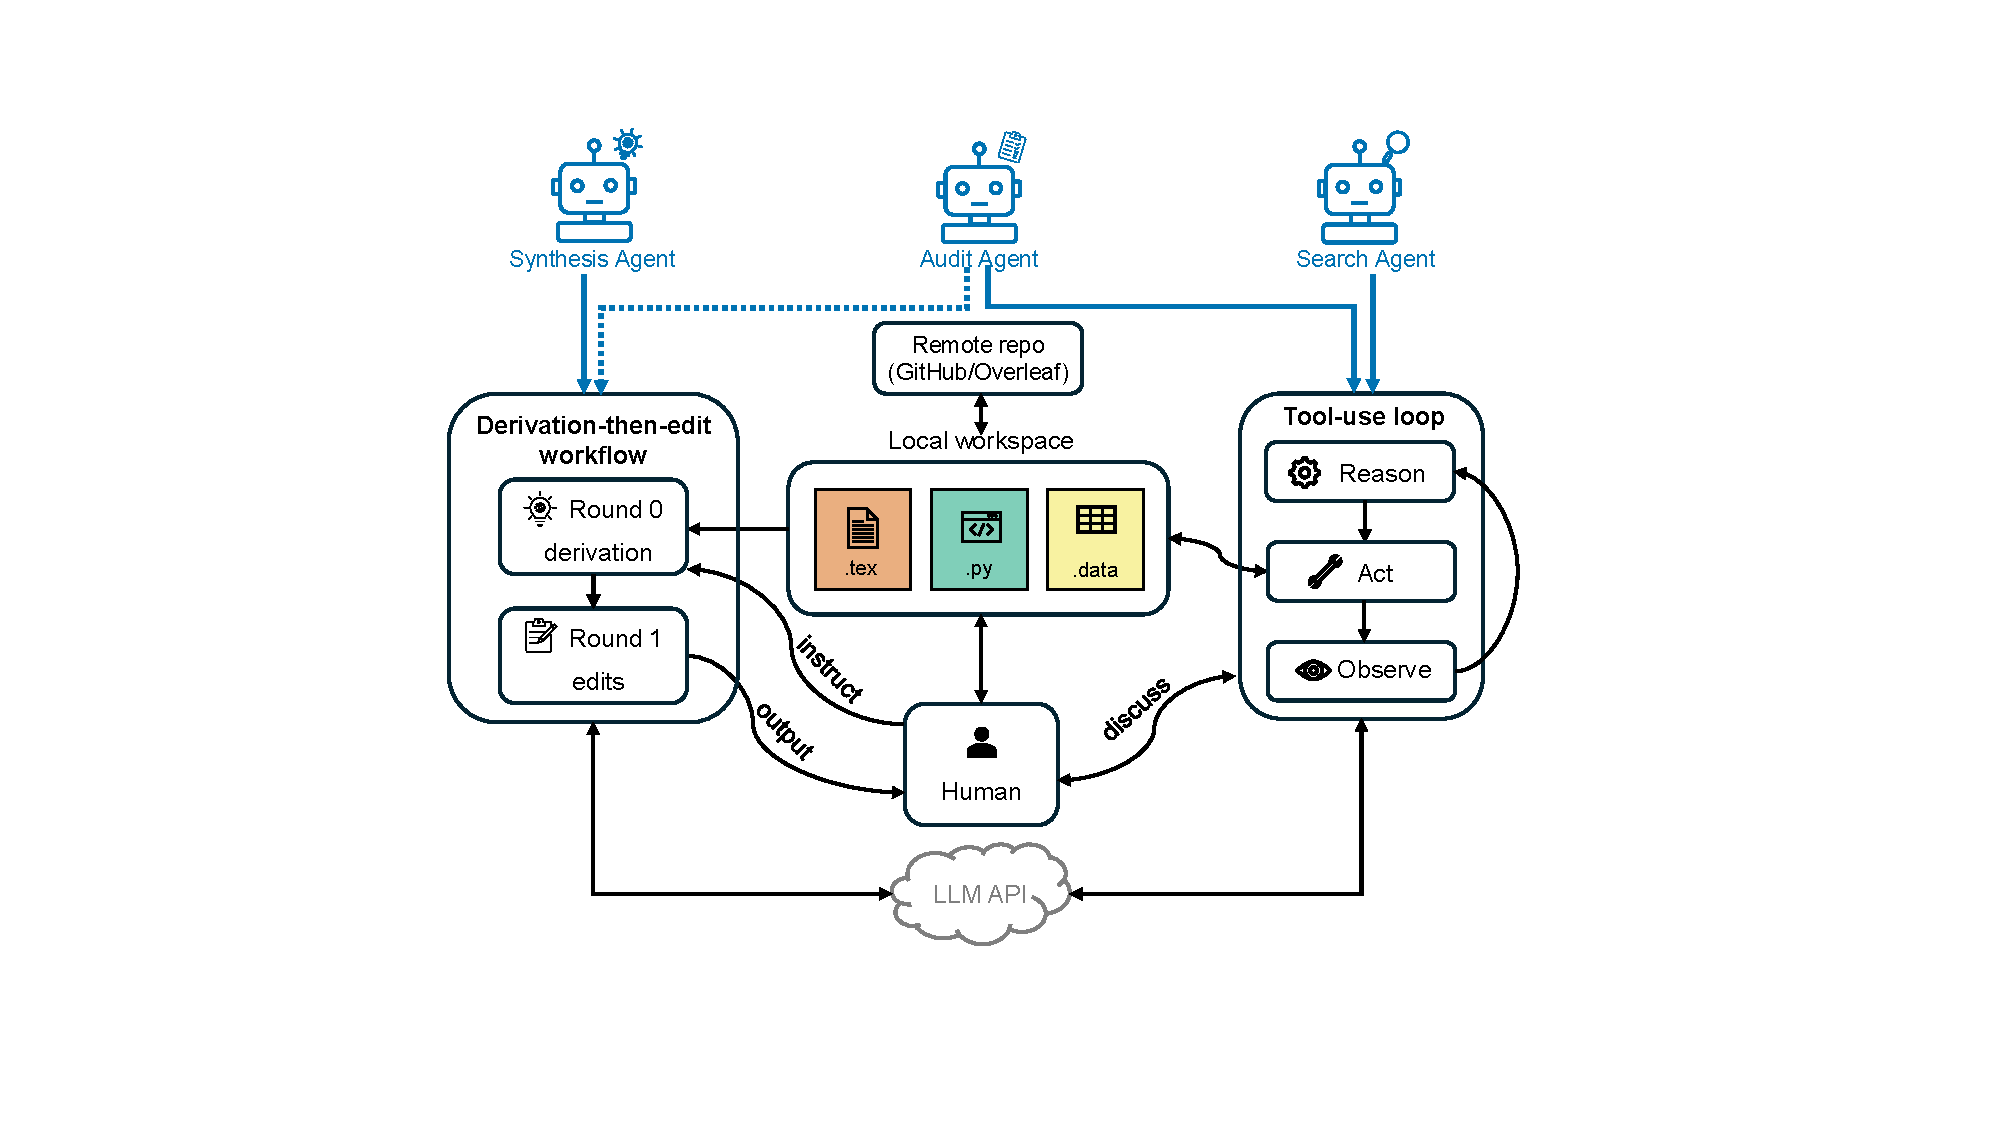
\includegraphics[width=0.95\linewidth]{Fig.2.pdf}
    \caption{TeXRA-enabled workspace linking agents, human, and tools. 
    All agents operate on a shared local project directory containing \LaTeX{} sources, Python scripts, and data files, synchronized with a remote repository (for example GitHub or Overleaf), and access a common large language model (LLM) backend via API. (a)~\emph{Derivation-then-edit workflow}: the Synthesis Agent produces an initial derivation (Round~0) and then refines or extends it in subsequent rounds, while the human and the Audit Agent review, instruct, and accept or reject suggested \LaTeX{} edits. (b)~\emph{Tool-use loop}: the Search Agent follows an iterative reason-act-observe (ReAct) cycle, writing and executing code to update the workspace under the verification of the Audit Agent, with the human able to intervene and discuss at any stage. Bidirectional arrows indicate interactive communication channels between the human and each agent.}
    \label{fig:agents-workspace}
\end{figure}

Given these capabilities, we structure a multi-agent architecture~\cite{Wu2023AutoGen,Du2023Improving,Sumers2023Cognitive} where specialized agents handle distinct subtasks under human orchestration. This separation provides \emph{specialization} (each agent focuses on one function with appropriate prompting), \emph{verification independence} (auditing agents do not see intermediate artifacts from generation agents), and natural \emph{checkpoints for human oversight} (we review proposals before committing to large computations and validate outputs to catch errors before they propagate).

\subsection{Combinatorial reformulation}
\label{subsec:comb}
The Synthesis Agent uses its LLM backend to recast the distance-2 construction in purely combinatorial terms. The key insight is that subset-sum residue classes can be used to simultaneously (i) enforce separation against single-bit flips and (ii) reduce the remaining $Z$-marginal constraints to a finite convex feasibility problem.

\paragraph{Residue separation implies distance two (screen).}
A key insight formulated by the agent is to use residue separation to satisfy the KL conditions for $X$ and $Y$ errors combinatorially. A single-bit flip at site $i$ maps a string $x$ to $x\oplus e_i$, which shifts its residue by $\pm w_i$ modulo $m$:
\[
    \langle \mathbf w, x\oplus e_i\rangle \equiv \langle \mathbf w, x\rangle \pm w_i \pmod m.
\]
Thus, to prevent all Hamming-1 adjacencies between the supports of different logical states, we can simply forbid residue differences that coincide with any $\pm w_i$. This leads to the lightweight screening condition:
\begin{equation}
    \label{eq:shift-screen-comb}
    S_j - S_k \ \not\equiv\ \pm w_i \pmod m \qquad \text{for every } i\in[n] \text{ and } j\neq k.
\end{equation}
When this condition holds, the classical union support $C$ has a minimum distance of $d(C)\ge 2$. As a result, all single-qubit $X/Y$ off-diagonal terms between distinct logical states vanish without any need for phase engineering.

(If some coordinate is pinned within a class, Eq.~\eqref{eq:shift-screen-comb} is sufficient but not necessary; an explicit $d(C)$ check may be substituted.)

\paragraph{$Z$ marginals as a finite convex intersection.}
Define the sign vector associated with a binary string $x$ as $v(x)\ :=\ ((-1)^{x_1},\dots,(-1)^{x_n})\in\{\pm1\}^n$. For each residue class $C_{S_j}(\mathbf w)$, let $V_j\ :=\ \{v(x):\ x\in C_{S_j}(\mathbf w) \}$ be the set of corresponding sign vectors. The set of all possible single-site $Z$-expectation vectors realizable by a state supported on class $j$ is precisely the convex hull of $V_j$, denoted $\operatorname{conv}(V_j)\subset[-1,1]^n$. The distance-2 KL equalities for the $Z_i$ operators are satisfied if and only if there exists a common expectation vector $q=(t_1,\dots,t_n)$ such that $q \in \bigcap_{j=0}^{K-1}\operatorname{conv}(V_j)$. This is equivalent to finding probabilities $\{p_{j,x}\}$ that satisfy:
\begin{equation}
    \label{eq:Zmatch-comb}
    \sum_{x\in C_{S_j}(\mathbf w)} (1-2x_i)\,p_{j,x}\ =\ t_i,
    \quad \forall i\in[n], \forall j,\qquad
    \text{with } \sum_{x\in C_{S_j}} p_{j,x}=1 \text{ and } p_{j,x}\ge 0.
\end{equation}
This reduction to a convex feasibility problem is the key simplification. Without residue separation, the KL conditions for $X/Y$ errors would couple the amplitudes $a_{j,x}$ and their phases quadratically across different residue classes, leading to large and ill-conditioned nonlinear systems. By enforcing $d(C)\ge 2$, we transform this intractable nonlinear problem into the tractable linear program of Eq.~\eqref{eq:Zmatch-comb}.

\paragraph{Small supports via Carath\'eodory's theorem.}
By Carath\'eodory's theorem~\cite{Caratheodory1907Uber} in $\mathbb{R}^n$, if the intersection $\bigcap_j\operatorname{conv}(V_j)$ is non-empty, then each class $j$ admits a solution supported on at most $n+1$ basis states. This guarantees that we can find sparse solutions. A convenient integer formulation of the feasibility problem is to find integer vectors $u_j$ and a common integer vector $t$ such that:
\begin{equation}
    \label{eq:int-feas-comb}
    A_j u_j\ =\ t,\qquad \mathbf 1^\top u_j\ =\ L\ \le\ n+1,\qquad
    u_j\ \in\ \mathbb{Z}_{\ge 0}^{|C_{S_j}|}\quad (\forall j),
\end{equation}
where $A_j$ is a matrix whose columns are the sign vectors $v(x)$ for $x\in C_{S_j}(\mathbf w)$. Normalizing by $L$ gives the rational solution $q=t/L$.

\paragraph{Fast no-go certificates.}
To efficiently prune the vast parameter space, the agent also formulates a method for generating fast no-go certificates. If $\bigcap_j \operatorname{conv}(V_j)=\varnothing$, the parameter set is infeasible. This is often witnessed by a linear separator: if there exist $\alpha\in\mathbb{Z}^n$ and $\beta\in\mathbb{R}$ such that
\[
\max_{x\in C_{S_j}} \alpha \cdot  v(x)\ <\ \beta\ <\ \min_{x\in C_{S_k}} \alpha \cdot  v(x)
\quad\text{for some } j\neq k,
\]
then the convex sets are strictly separated, and Eq.~\eqref{eq:Zmatch-comb} is impossible. Computing $\alpha \cdot v(x)$ is extremely fast, allowing us to use such separators to reject large portions of the $(m,\mathbf w,\mathbf S)$ search space before attempting a full LP solve.

\paragraph{Two illustrative patterns.}
\emph{Homogeneous weights.} If $\mathbf w=(t,\dots,t)$ with $\gcd(t,m)=1$, then $C_{S_j}(\mathbf w)$ coincides with Hamming-weight layers modulo $m$:
\[
    C_{S_j}(\mathbf w)=\bigl\{x:\ \mathrm{wt}(x)\equiv S_j\,t^{-1}\ (\bmod\ m) \bigr\}.
\]
For small $n$ and multiple distinct layers, the screen Eq.~\eqref{eq:shift-screen-comb} typically forces an extreme layer (e.g.\ $\mathrm{wt}=0$ or $n$), which pins $V_j$ to $\{\pm(1,\dots,1)\}$ and often prevents a common $q$ with the same parity $L\le n+1$ across the remaining layers.
\emph{Mixed weights (affine slices).} For many $\mathbf w$, the congruence fixes $\sum_{i\in I} x_i$ modulo $m$, so $V_j$ lies in an affine slice
$\{\mu\in[-1,1]^n:\ \sum_{i\in I}\mu_i=c_j'\,\}$ with different constants $c_j'$.
If these slices share no rational point with denominator $\le n+1$, a linear functional separates them, yielding an immediate no-go.

\subsection{Search space and enumeration pipeline}
\label{subsec:search}

We now describe how the SSLP formulation is instantiated at scale to enumerate codes with transversal diagonals and distance $2$.

\subsubsection{Canonical search space and guards}

To avoid redundant enumeration, we restrict to canonical representatives. The Search Agent enumerates weight vectors $\mathbf w$ in non-decreasing order
\[
  1\le w_1\le\cdots\le w_n\le m-1,
\]
and residue tuples $\mathbf S$ with $S_0=0$ and
\[
  1\le S_1<\cdots<S_{K-1}\le m-1.
\]
Equivalence under qubit permutations is tracked so that each discovered code is genuinely distinct. Two lightweight guards are applied before any heavy computation:
(i) an optional coprime filter on the residues $S_j$, and
(ii) the residue-shift screen condition
\begin{equation}
    \label{eq:shift-screen-comb}
    S_j - S_k \ \not\equiv\ \pm w_i \pmod m \qquad \text{for every } i\in[n] \text{ and } j\neq k,
\end{equation}
which forbids all Hamming-1 adjacencies between supports of different logical states.

\subsubsection{Supports, union distance, and Z-only feasibility}

For each parameter set $(\mathbf w,m,\mathbf S)$ that passes the initial guards, we construct the residue classes $C_{S_j}(\mathbf w)$ by evaluating
$\langle \mathbf w,x\rangle \bmod m$ for all $x\in\{0,1\}^n$. Any set for which a class $C_{S_j}(\mathbf w)$ is empty is discarded.

We then compute the minimum distance of the union support,
\begin{equation}
  C :=\bigcup_{j=0}^{K-1} C_{S_{j}}(\mathbf w),\qquad
  d(C)=\min_{\substack{x\ne y\\x,y\in C}} d_{\mathrm H}(x,y).
  \label{eq:distance2}
\end{equation}
For the catalogue reported in the main text we impose $d(C)=2$, consistent with the distance-2 setting; in large sweeps we often rely on Eq.~\eqref{eq:shift-screen-comb} as a fast sufficient condition and only compute $d(C)$ for promising candidates.

Next, we test $Z$-only feasibility by solving the linear program implied by Eq.~\eqref{eq:Zmatch-comb}. Let $p_{j,x}$ denote non-negative, block-normalized probabilities on $C_{S_j}(\mathbf w)$ such that
$\langle j_{L} |Z_i| j_{L} \rangle=\sum_{x\in C_{S_j}(\mathbf{w})} p_{j,x}(1-2x_i)$. The KL equalities for all $Z_i$ are satisfied if there exists a set $\{p_{j,x}\}$ obeying
\begin{equation}
  \begin{split}
    &\sum_{x\in C_{S_0}(\mathbf{w})} p_{0,x} (1-2x_i)
      = \sum_{y\in C_{S_j}(\mathbf{w})} p_{j,y} (1-2y_i),
      \qquad \forall i\in[n],\ \forall j=1,\dots,K-1,\\
    &\sum_{x\in C_{S_j}(\mathbf{w})} p_{j,x} = 1,\qquad
      p_{j,x}\ge 0\quad \forall j,\ \forall x\in C_{S_j}(\mathbf{w}).
  \end{split}
  \label{eq:Zmatch}
\end{equation}
We assemble these into a block-structured linear system $A_{\mathrm{eq}} \mathbf{p}=b_{\mathrm{eq}}$ with $\mathbf{p}\ge 0$, where $\mathbf{p}$ concatenates all $p_{j,x}$. For $K=2$, this is an $(n+2)\times(|C_{S_0}|+|C_{S_1}|)$ system. We solve Eq.~\eqref{eq:Zmatch} numerically using standard LP solvers and then convert numerical solutions to exact rationals as described below.

\subsubsection{Rational reconstruction}
\label{subsubsec:rational-main}

Although $A_{\mathrm{eq}}$ and $b_{\mathrm{eq}}$ are integer-valued, the LP solver operates in floating-point arithmetic, and naive rounding of the resulting $\mathbf p^{(\mathrm{num})}$ can violate the constraints. To obtain exact rational solutions $\mathbf p\in\mathbb Q^N$ we exploit the underlying integer structure in two complementary ways.

First, when the solution is close to a basic feasible solution (BFS), at most $(K-1)n+K$ entries are nonzero. We then identify a full-rank basis $B$ of that size, form the integer submatrix $A_B\in\mathbb{Z}^{((K-1)n+K)\times((K-1)n+K)}$, and solve
$A_B \mathbf{p}_B=b_{\mathrm{eq}}$ exactly over $\mathbb Q$, with $p_i=0$ for $i\notin B$. The resulting vector $\mathbf{p}$ is accepted if $A_{\mathrm{eq}}\mathbf{p}=b_{\mathrm{eq}}$ and $\mathbf{p}\ge 0$ hold exactly.

Second, when the numerical solution is not clearly a BFS, we first rationalize each coordinate by continued fractions (imposing a denominator bound) and then project back onto the affine constraint space $A_{\mathrm{eq}}\mathbf p=b_{\mathrm{eq}}$ using exact rational linear algebra. Small negative entries caused by rounding are clipped to $0$ and the vector is re-projected and block-normalized. Detailed pseudocode for these two procedures is given in Supplementary Algorithms~\ref{alg:exactbfs-supp}–\ref{alg:ratproj-supp}~\cite{Bareiss1968Sylvester,Bertsimas1997Introduction,Schrijver1986Theory,Vonzurgathen2003Modern,Lenstra1982Factoring,Ferguson1999Analysis}.


\subsubsection{Search skeleton and recorded outputs}

The full search procedure over $(m,\mathbf w,\mathbf S)$ can be summarized as follows:
(i) enumerate canonical $(\mathbf w,\mathbf S)$ subject to initial guards;
(ii) construct residue classes and enforce non-emptiness;
(iii) check the distance-2 screen (either via Eq.~\eqref{eq:shift-screen-comb} or by computing $d(C)$);
(iv) solve the $Z$-only LP Eq.~\eqref{eq:Zmatch};
(v) perform rational reconstruction;
(vi) assemble logical states and verify all distance-2 KL conditions and the transversal logical action.

For each successful hit we record $(n,m,K,\mathbf w,\mathbf S)$, the rational probabilities $\{p_{j,x}\}$, the explicit logical states $\{\ket{j_L}\}$, the per-site expectations $\langle Z_i\rangle$, and the logical order $\mathcal O$.

\subsection{Verification protocol and audit agent}
\label{subsec:audit}

The Search Agent produces candidate codes with claimed parameters and logical actions. To ensure correctness, we maintain an independent verification pipeline managed by the Audit Agent, supplemented by manual checks.

\subsubsection{Reconstructing states and checking KL conditions}

Given a record
$R=(n,m,\mathbf w,\mathbf S,\{C_{S_j}(\mathbf w)\}_{j=0}^{K-1},\{p_{j,x}\})$
with $\sum_{x\in C_{S_j}}p_{j,x}=1$, the Audit Agent reconstructs logical states as
\[
  \ket{j_{L}}=\sum_{x\in C_{S_j}(\mathbf{w})}\sqrt{p_{j,x}} \ket{x}.
\]
It then checks two sets of conditions for each site $i$ and each Pauli $P_i\in\{X_i,Y_i,Z_i\}$:
(i) equal diagonals,
$\langle j_{L}|P_i| j_{L} \rangle=\langle k_{L} |P_i| k_{L} \rangle$ for all $j,k$;
and (ii) vanishing off-diagonals,
$\langle j_{L} | P_i | k_{L} \rangle=0$ for all $j \neq k$.
These checks are performed in both floating-point arithmetic (with a numerical tolerance) and exact rational arithmetic ($\tau=0$).

\subsubsection{Verifying transversal logical actions}

To verify the logical action of the transversal gate $U(\mathbf w,m)$, the Audit Agent applies $U(\mathbf w,m)$ to each logical state and computes the overlap
$\braket{j_L | U(\mathbf w,m) | j_L}$. This projection must yield the expected eigenvalue $\omega_m^{S_j}$ and confirm that $U(\mathbf w,m)\ket{j_L}$ is proportional to $\ket{j_L}$. Any deviation beyond numerical tolerance triggers rejection of the candidate.

\subsubsection{Independent implementations and manual audit}

The Audit Agent is prompted with the verification rules and independently generates a Python checker for the search results. For all new quantum codes found for $n\in\{4,5,6\}$, this automated audit passed. In addition, the researcher implemented an independent verifier and re-ran all checks on the final catalogue.

Manual validation consists of two components: (i) re-running KL and transversal checks with independently written scripts and libraries, and (ii) spot-checking representative instances (including those used to define analytical families) by hand, verifying both the combinatorial screens and the $Z$-marginal equalities.

\subsection{Proof outlines for analytical families and residue-degenerate codes}
\label{subsec:families-methods}

We provide brief proof outlines for the analytical families and residue-degenerate constructions discussed in the main text. Full derivations and explicit small-$n$ instances are given in Supplementary Notes~\ref{supp:families-examples} and~\ref{supp:degenerate-642}.


\subsubsection{Family I: $C_0=\{0^n,1^n\}$}
\label{subsubsec:proof_family_1}

Fix $n\ge 2$, a modulus $m\ge n$, and
\[
  \mathbf w=(1,1,\dots,1,m-(n-1))\in(\mathbb Z_m)^n.
\]
Define residue classes
$C_s=\{x\in\{0,1\}^n : \langle \mathbf w,x\rangle \equiv s \pmod m\}$.

Writing $x=(u,b)$ with $u\in\{0,1\}^{n-1}$, $b\in\{0,1\}$ and $t=\mathrm{wt}(u)$, we obtain
$\langle \mathbf w,x\rangle\equiv t + b(m-(n-1)) \pmod m$. For $m\ge n$, the residue-$0$ class contains only $0^n$ and $1^n$, so $C_0=\{0^n,1^n\}$. For $1\le s\le m-1$ in a suitable window, $C_s$ decomposes into two Hamming-weight slices $A_s$ and $B_t$ supported on $b=0$ and $b=1$, respectively, where $t=n-1+s-m$.

Choosing $\ket{0_L}$ supported on $C_0$ and $\ket{1_L}$ supported on $C_s$, a symmetric solution of the $Z$-marginal constraints assigns probabilities
\[
  p(0^n)=1-\frac{s}{m},\qquad p(1^n)=\frac{s}{m}
\]
on $C_0$ and
\[
  q(y)=
  \begin{cases}
    \dfrac{m-s}{m}\,\dfrac{1}{\binom{n-1}{s}}, & y\in A_s,\\[4pt]
    \dfrac{s}{m}\,\dfrac{1}{\binom{n-1}{t}},   & y\in B_t,
  \end{cases}
\]
on $C_s$, giving a common single-site expectation
$\langle Z_i\rangle=1-2s/m$ for all $i$. The transversal
$U(\mathbf w,m)$ then acts as
$\overline U=\mathrm{diag}(1,\omega_m^s)$, with logical order
$m/\gcd(m,s)$. Imposing the shift screen
$s\not\equiv\pm1,\pm(m-(n-1))\pmod m$ guarantees that all weight-1 $X/Y$ matrix elements vanish combinatorially, so the code has distance~2. Explicit examples for small $n$ are listed in Supplementary Note~\ref{supp:families-examples}.


\subsubsection{Family II: even-parity subset-sum codes}
\label{subsubsec:proof_family_2}
Let $n$ be even and
$\mathsf E=\{\sigma\in\{0,1\}^n:\mathrm{wt}(\sigma)\equiv 0\ (\mathrm{mod}\ 2)\}$ denote the even-parity subcode. For modulus $m$, weights $\mathbf w\in(\mathbb Z_m)^n$, and residues $\mathbf S=\{S_0,\dots,S_{K-1}\}\subset\mathbb Z_m$ with $S_0=0$, define
\[
  C^{(+)}_{S_k}(\mathbf w)
  =\Bigl\{\sigma\in\mathsf E:\textstyle\sum_{j=1}^n w_j\sigma_j\equiv S_k\pmod m\Bigr\},
\]
and logical states
\[
  \ket{k_L}=\frac{1}{\sqrt{|C^{(+)}_{S_k}|}}\sum_{\sigma\in C^{(+)}_{S_k}}\ket{\sigma},\quad k=0,\dots,K-1.
\]

Every $\ket{k_L}$ is supported entirely on even-parity strings, so any single $X_i$ or $Y_i$ error maps basis states to odd-parity strings outside the union of supports. Thus all $X/Y$ matrix elements vanish identically. For the $Z$-error constraints it suffices to enforce \emph{column balance}: for each class $k$ and each site $i$, exactly half of the strings in $C^{(+)}_{S_k}$ have a $1$ at position $i$. In that case
$\langle k_L|Z_i|k_L\rangle=0$ for all $k$, and disjoint supports imply $\langle k_L|Z_i|\ell_L\rangle=0$ for $k\neq\ell$, so the KL conditions hold and the code has distance~2. The diagonal transversal $U(\mathbf w,m)$ acts as
$\overline U=\mathrm{diag}(\omega_m^{S_0},\dots,\omega_m^{S_{K-1}})$ with logical order
$\mathcal O=m/\gcd(m,S_1,\dots,S_{K-1})$. The instances summarized in the catalogue correspond to parameter choices where each $C^{(+)}_{S_k}$ is closed under an involutive symmetry (e.g. bitwise complement or structured pairings), which guarantees column balance; see Supplementary Note~\ref{supp:families-examples} for full listings.


\subsubsection{Residue-degenerate \texorpdfstring{$((6,4,2))$}{((6,4,2))} controlled-phase code}
\label{subsubsec:proof_642}

Finally, we outline the residue-degenerate $((6,4,2))$ controlled-phase code used in the main text as an example of relaxing residue nondegeneracy. A full derivation and explicit computational-basis expansions are given in Supplementary Note~\ref{supp:degenerate-642}.

We work with modulus $m=4$ and weight vector
\[
  \mathbf w=(1,3,2,2,2,2)\in\mathbb Z_4^6.
\]
For $x=(x_1,\dots,x_6)$ the residue is
\[
  \operatorname{res}(x)\equiv \mathbf w\cdot x \pmod 4
  = x_1 - x_2 + 2\,(x_3\oplus x_4\oplus x_5\oplus x_6)\pmod 4,
\]
so it is determined by $(x_1,x_2)$ and the parity of the last four bits. We organize the last four qubits into even- and odd-parity subsets indexed by $t\in\mathbb F_2^3$ via
\[
  \phi(t)=(t_1,t_2,t_3,t_1\oplus t_2\oplus t_3) \quad\text{(even parity)},
\]
\[
  \psi(t)=(t_1,t_2,t_3,1\oplus t_1\oplus t_2\oplus t_3) \quad\text{(odd parity)}.
\]
Defining characters
$\chi_3(t)=(-1)^{t_1}$, $\chi_4(t)=(-1)^{t_2}$, $\chi_5(t)=(-1)^{t_3}$ and sign patterns
\[
  s_0(t)=1,\qquad s_1(t)=\chi_3(t)\chi_4(t),\qquad s_2(t)=\chi_3(t)\chi_5(t),
\]
we construct three residue-$0$ logical states
\[
  \ket{j_L}
    =\frac{1}{4}\sum_{t\in\mathbb F_2^3} s_j(t)\bigl(\ket{00\,\phi(t)}+\ket{11\,\phi(t)}\bigr),
    \quad j=0,1,2,
\]
and a residue-$1$ state
\[
  \ket{3_L}
    =\frac{1}{4}\sum_{t\in\mathbb F_2^3} \chi_5(t)\bigl(\ket{10\,\phi(t)}+\ket{01\,\psi(t)}\bigr).
\]
Each logical state contains $16$ basis strings with amplitudes of modulus $1/4$, so all are normalized; disjoint residues imply $\ket{3_L}$ is orthogonal to the residue-$0$ block, while character orthogonality on $\mathbb F_2^3$ ensures orthogonality within $\{\ket{0_L},\ket{1_L},\ket{2_L}\}$.

For qubits $3$–$6$, any bit flip toggles the parity of the last four bits and shifts the residue by $2$, mapping supports to residue values $2$ or $3$ that are unoccupied; hence all $X_i/Y_i$ matrix elements with $i\in\{3,4,5,6\}$ vanish. For $Z_i$ on the last four qubits, each logical state has a $50/50$ split of $0$ and $1$ in coordinate $i$, so the diagonals vanish, and off-diagonals reduce to averages of nontrivial characters, which vanish by orthogonality. For qubits $1$ and $2$, the patterns $(00)$, $(11)$, $(10)$, and $(01)$ are arranged so that $X_1,X_2,Y_1,Y_2$ map between residue classes without producing overlap with any logical support, while $Z_1,Z_2$ diagonals and off-diagonals cancel by symmetry. Altogether, all weight-1 KL equations are satisfied and the code has distance $2$.

The transversal operator
\[
  U=\bigotimes_{j=1}^6 Z\!\left(\tfrac{\pi}{2} w_j\right)
\]
acts as $U\ket{x}=i^{\mathbf w\cdot x}\ket{x}=i^{\operatorname{res}(x)}\ket{x}$, so it contributes a constant phase to each residue class. Since $\ket{0_L},\ket{1_L},\ket{2_L}$ lie entirely in residue value $0$ and $\ket{3_L}$ lies in residue value $1$, we obtain the logical action
\[
  U_L=\mathrm{diag}(1,1,1,i)
\]
on the ordered logical basis. This construction lies outside the strictly nondegenerate residue regime used in our systematic sweeps and illustrates how relaxing that guard yields a new $((6,4,2))$ code with a non-trivial diagonal transversal gate.







\section*{Data availability}
The catalogue of quantum codes discovered in this work, including all parameters, logical states, and verification results, is available at [repository URL to be added upon publication].
% The data used to generate figures are included in the Supplementary Information.

\section*{Code availability}
The Python code for the SSLP search pipeline, rational reconstruction algorithms, and verification routines is available at [repository URL to be added upon publication].
The multi-agent system was implemented using the TeXRA platform~\cite{Texra2025TeXRA} with the GPT-5 API~\cite{Openai2025GPT}.

\section*{Author contributions}
X.H.\ implemented the search, screening, rational reconstruction and verification procedure, performed the experiments. S.L.\ %designed TeXRA and 
contributed to the agent development and tooling, helped formulate the analytical derivations. B.Z.\ conceived and developed the multi-agent workflow, supervised the project, provided research direction. All authors contributed to analyzing results and writing the manuscript.

\section*{Competing interests}
The authors declare no competing interests.

\section*{Acknowledgements}
The authors would like to express their gratitude to Alexander Frei and Ningping Cao for helpful
discussions.


\begin{appendices}

%\section{Section title of first appendix}\label{secA1}

%An appendix contains supplementary information that is not an essential part of the text itself but which may be helpful in providing a more comprehensive understanding of the research problem or it is information that is too cumbersome to be included in the body of the paper.



\section{Additional background on the SSLP framework and transversal gates}
\label{sec:addi}

We briefly summarize the error-correction setting, subset-sum notation, and transversal gates that underlie the SSLP framework. These definitions were provided to the agents as seed input, partially synthesized and adapted from Ref.~\cite{Zhang2025Transversal} using the derivation-then-edit workflow described in Sec.~\ref{subsec:workspace}.

\subsection{Basic notations and definitions}
\label{subsec:notation}

We work on an $n$-qubit system with computational basis $\{\ket{x}: x\in\{0,1\}^n\}$, where $x=(x_1,\ldots,x_n)$ and $\ket{x}\equiv\ket{x_1}\otimes\cdots\otimes\ket{x_n}$. The Hamming weight is $\mathrm{wt}(x)=\sum_i x_i$, and the Hamming distance is $d_{\mathrm{H}}(x,y)=\mathrm{wt}(x\oplus y)$. The single-qubit Pauli operators are
\[
    X=\begin{bmatrix}0&1\\1&0\end{bmatrix},\quad
    Y=\begin{bmatrix}0&-i\\i&0\end{bmatrix},\quad
    Z=\begin{bmatrix}1&0\\0&-1\end{bmatrix},
\]
where $Z_i$ acts on a basis state as $Z_i\ket{x}=(-1)^{x_i}\ket{x}$. We denote code parameters by $((n,K,d))$~\cite{Nielsen2010Quantum}, for $n$ physical qubits, a code dimension of $K$, and a distance of $d$. We use the standard notation $[n]:=\{1,\ldots,n\}$ for index sets.

A quantum code with distance $d$ encodes information into a $K$-dimensional subspace spanned by orthonormal logical states $\{\ket{j_L}\}_{j=0}^{K-1}$. The KL conditions~\cite{Knill1997Theory} ensure error detectability: for a set $\mathcal{E}$ of detectable errors, $\bra{j_L}E^\dagger E'\ket{j'_L}=0$ when $j\neq j'$, and $\bra{j_L}E^\dagger E'\ket{j_L}=\lambda_{E,E'}$ is independent of $j$.

For distance $d=2$, we take the set of detectable errors to be $E_D=\{X_i,Y_i,Z_i:\ i\in[n]\}$ (all single-qubit Paulis). The KL conditions~\cite{Knill1997Theory} simplify to
\begin{align}
    \bra{j_L}P_i\ket{j'_L} &=0\ \text{for } j\neq j',\notag\\
    \bra{j_L}P_i\ket{j_L}  &=\lambda_{P_{i}} \quad \text{for all } j \in \{ 0, \dots, K-1\},
    \label{eq:KL-d2}
\end{align}
for all $P_i\in\{X_i,Y_i,Z_i\}$, where the scalars $\lambda_{P_i}$ are independent of the logical state $j$. Writing a logical state as $\ket{j_L}=\sum_x a_{j,x}\ket{x}$ with probabilities $p_{j,x}=|a_{j,x}|^2$, the diagonal constraints for $Z_i$ become
\begin{equation}
    \sum_x (1-2x_i)p_{j,x} = t_i \quad \text{for all } i\in[n], j=0,\ldots,K-1,
    \label{eq:Z-KL}
\end{equation}
for some site-wise constants $t_i\in\mathbb{R}$. The constraints for $X_i$ and $Y_i$ involve cross-terms of the form $a_{j,x}^* a_{j',x\oplus e_i}$ between Hamming-1 neighbors, which couple the amplitudes nonlinearly.

In addition, the definitions of the quantum weight enumerator and signature vector are presented as follows.

\begin{definition}[Quantum weight enumerators]\label{def:weight-enumerator}
Let $\Pi$ be the projector onto an $((n,K,d))$ quantum code, and let $\mathcal P_n$ denote the $n$-qubit Pauli group
generated by $\{I,X,Y,Z\}^{\otimes n}$ (up to overall phases). 
Following Rains' distance-two analysis and subsequent work~\cite{Rains2002Quantum,Du2024Characterizing,Zhang2025Transversal}, 
the quantum weight enumerators associated with $\Pi$ are the polynomials
\[
  A(z) \;=\; \sum_{j=0}^n A_j z^j,
  \qquad
  B(z) \;=\; \sum_{j=0}^n B_j z^j,
\]
with coefficients
\begin{align*}
  A_j &\;=\; \frac{1}{K^2} 
    \sum_{\substack{E\in\mathcal P_n \\ \mathrm{wt}(E)=j}}
      \Bigl|\mathrm{Tr}(\Pi E)\Bigr|^2, \\
  B_j &\;=\; \frac{1}{K} 
    \sum_{\substack{E\in\mathcal P_n \\ \mathrm{wt}(E)=j}}
      \mathrm{Tr}\!\bigl(\Pi E \Pi E^\dagger\bigr).
\end{align*}
Here $\mathrm{wt}(E)$ is the Pauli weight, i.e.\ the number of non-identity tensor factors in $E$.
The sequences $A=(A_0,\dots,A_n)$ and $B=(B_0,\dots,B_n)$ are invariants of the code under local unitaries.
\end{definition}

\begin{definition}[Signature vector and signature norm $\lambda^*$]\label{def:signature-norm}
Let $E_{\mathrm D}$ be the detectable Pauli error set used in the KL conditions for the code (for the distance-$2$ setting in this work one may take $E_{\mathrm D}=\{X_i,Y_i,Z_i : i\in[n]\}$, cf.\ Sec.~2.2).
For each $E\in E_{\mathrm D}$, let $\lambda_E \in \mathbb C$ be the corresponding KL coefficient, characterized by
$\Pi E \Pi = \lambda_E \Pi$ and equivalently $\lambda_E = \tfrac{1}{K}\mathrm{Tr}(\Pi E)$.
The signature vector on $E_{\mathrm D}$ is
\[
  \tilde\lambda \;:=\; (\lambda_E)_{E\in E_{\mathrm D}} \;\in\; \mathbb C^{|E_{\mathrm D}|},
\]
and its Euclidean norm
\[
  \lambda^* \;:=\; \|\tilde\lambda\|_2 \;=\;
  \Biggl(\sum_{E\in E_{\mathrm D}} |\lambda_E|^2\Biggr)^{1/2}
\]
is called the signature norm of the code~\cite{Du2024Characterizing,Zhang2025Transversal}. 
In particular, for the Pauli error models considered in this work, $\lambda^*$ is a scalar invariant that summarizes how the code projector overlaps with the detectable error operators.
\end{definition}































\subsection{Subset-sum classes and modular inner product}
\label{subsec:residue-classes}

Fix a modulus $m\in\mathbb{Z}_{>0}$ and a weight vector $\mathbf w=(w_1,\dots,w_n)\in(\mathbb{Z}_m)^n$. We define the modular inner product as
\[
    \langle \mathbf w,x\rangle \equiv \sum_{i=1}^n w_i x_i \pmod m,
\]
and the corresponding residue classes as
\begin{equation}
    C_{S_{j}}(\mathbf w):=\{x\in\{0,1\}^n:\ \langle \mathbf w,x\rangle\equiv S_{j} \pmod m \}, \quad \text{for } j=0, \cdots, K-1.
    \label{eq:res-class-pre}
\end{equation}
Throughout this paper, we require each logical basis state to be supported on a single such class: $\mathrm{supp}(\ket{j_L})\subseteq C_{S_j}(\mathbf w)$ for a set of residues $\mathbf S=(S_0,\dots,S_{K-1})\in(\mathbb{Z}_m)^K$. We take $S_0=0$ without loss of generality. Let $C:=\bigcup_{j}C_{S_j}(\mathbf w)$ denote the classical union support of the code, and let $d(C):=\min_{x\neq y\in C} d_{\mathrm{H}}(x,y)$ be its minimum distance.

\subsection{Transversal diagonals and logical order}
\label{subsec:transversals}

We consider the phase gate
\[Z(\theta)=\mathrm{diag}(1,e^{i\theta}),\]
and define the transversal operator
\begin{equation}
    U(\mathbf w,m):=\bigotimes_{i=1}^n Z \left(\tfrac{2\pi w_i}{m}\right),\qquad
    U(\mathbf w,m)\ket{x}= \omega_m^{\langle \mathbf w,x\rangle}\ket{x}, \
    \text{where } \omega_m=e^{2\pi i/m}.
    \label{eq:U-pre}
\end{equation}
If $\mathrm{supp}(\ket{j_L})\subseteq C_{S_j}(\mathbf w)$, then $U(\mathbf w,m)$ acts diagonally on the logical basis:
\begin{equation}
    U(\mathbf w,m)\ket{j_L}=\omega_m^{S_j}\ket{j_L},\qquad
    \overline U=\mathrm{diag}(\omega_m^{S_0},\dots,\omega_m^{S_{K-1}}),
    \label{eq:logical-diag-pre}
\end{equation}
The (projective) order of the induced cyclic logical group is
\begin{equation}
    \mathcal O=\frac{m}{\gcd(m,S_1,\dots,S_{K-1})}.
    \label{eq:order-pre}
\end{equation}
Using the rotation gate $R_Z(\theta)=e^{-i\theta Z/2}$ instead only introduces a global phase, leaving relative logical phases invariant; however, the absolute order of the logical cyclic group can double~\cite{Zhang2025Transversal}.

\subsection{Subset-sum linear program (SSLP)~\cite{Zhang2025Transversal} for distance-2 codes}
\label{subsec:sslp}

Given parameters $(n,K,m,\mathbf w,\mathbf S)$, where $\mathbf w=(w_1,\dots,w_n)\in(\mathbb Z_m)^n$ and $\mathbf S=\{S_0,\dots,S_{K-1}\}\subset\mathbb Z_m$ (with $S_0=0$), the SSLP framework consists of three main steps:

\paragraph{Step 1: Determining Logical-State Support Subsets.}
Compatibility with the transversal gate $U(\mathbf w,m)$ forces each logical basis state $\ket{j_L}$ to be supported exclusively on a single residue class:
\[
    \mathrm{supp}(\ket{j_L}) \subseteq C_{S_j}(\mathbf w):=\bigl\{x\in\{0,1\}^n:\ \langle \mathbf w,x\rangle \equiv S_j \pmod m \bigr\}.
\]
If the residues $\{S_j\}$ are distinct, the supports $C_{S_j}(\mathbf w)$ are disjoint, which ensures orthogonality and dramatically simplifies the search.


\paragraph{Step 2: Linear-Programming Filter from Z-type KL Conditions.}
We introduce non-negative probabilities $p_{j,x}=|a_{j,x}|^2$ for each logical state $j$, defined on its support $C_{S_j}(\mathbf w)$ and normalized such that $\sum_{x\in C_{S_j}} p_{j,x}=1$. The single-site $Z$-marginal equalities require the existence of site parameters $t_i\in\mathbb R$ such that
\[
    \sum_{x\in C_{S_j}(\mathbf w)} (1-2x_i)\,p_{j,x} =  t_i,
    \qquad \forall\, i=1,\dots,n,\ \forall\, j=0,\dots,K-1,
\]
along with the non-negativity constraints $p_{j,x}\ge 0$. This is a linear feasibility program; any parameter set $(\mathbf w,\mathbf S)$ for which this program is infeasible can be discarded immediately.


\paragraph{Step 3: Solving for the remaining KL conditions.}
With supports fixed (Step 1) and $Z$-type marginals feasible (Step 2), we now solve for complex amplitudes $a_{j,x}$ so that the \emph{full} KL equalities hold for errors beyond the $Z$-only case. This can be done by minimizing a differentiable KL loss on the Stiefel manifold as shown in~\cite{Zhang2025Transversal}. Because $X$ (and $Y$) errors map $C_{S_j}$ into $C_{S_j\pm w_i}$, these terms couple distinct residue blocks, making the problem nonconvex and globally coupled. In practice, this stage is the computational bottleneck: solutions are typically numerical, hard to verify analytically, and difficult to scale to larger $n$.

\paragraph{Worked example.}
A detailed instantiation of this SSLP pipeline on a $((5,2,2))$ example, including explicit residue classes, linear system, and rational solution family, is provided in Supplementary Note~\ref{supp:example-522}. This example was part of the seed input given to the agents.

%%%%%%%%%%%%%%%%%%%%%%%%%%%%%%%%%%%%%%%%%%%%%%%%%%%%%%%%%%%%%



%%%%%%%%%%%%%%%%%%%%%%%%%%%%%%%%%%%%%%%%%%%%%%%%%%%%%%%
\section{Detailed \texorpdfstring{$((5,2,2))$}{((5,2,2))} SSLP example}
\label{supp:example-522}

In this note we give a step-by-step derivation of the $((5,2,2))$ example that was used to seed the multi-agent system. It instantiates the subset-sum linear program (SSLP) in the distance-2 regime and illustrates how residue separation and $Z$-only feasibility interact.

\subsection{Parameters}

We consider
\[
    n=5,\quad \mathbf w=(1,1,2,2,2)\ \text{(sorted nondecreasingly)},\quad
    m=7,\quad K=2,\quad (S_0,S_1)=(0,4).
\]
For $S\in\{0,4\}$ we define the residue class
\[
    C_{S}(\mathbf w):=\{x\in\{0,1\}^5:\ \langle\mathbf w,x\rangle\equiv S \pmod 7\},
\]
where
$\langle\mathbf w,x\rangle\equiv \sum_{i=1}^5 w_i x_i \pmod 7$.

We impose the design condition that the classical union support
\[
    C:=C_{S_0}(\mathbf w)\cup C_{S_1}(\mathbf w)
\]
has minimum Hamming distance
\[
    d(C)=2.
\]
This forbids any Hamming-1 neighbours anywhere in $C$; as a consequence, all single-qubit $X_i/Y_i$ off-diagonal Knill--Laflamme (KL) constraints vanish automatically.

\paragraph{Step 1: Subset-sum supports}

Direct enumeration of $\langle\mathbf w,x\rangle\bmod 7$ for all $x\in\{0,1\}^5$ yields:
\[
    \begin{aligned}
        C_{S_0}(\mathbf w)=C_0 & =\{00000, 01111, 10111\},\\
        C_{S_1}(\mathbf w)=C_1 & =\{00011, 00101, 00110, 11001, 11010, 11100\}.
    \end{aligned}
\]
These are the basis strings that may carry nonzero amplitudes in the logical states.

\paragraph{Step 2: Enforcing classical distance}

The classical union $C=C_0\cup C_1$ satisfies $d(C)=2$: no two distinct strings in $C$ differ by Hamming distance $1$. Therefore, for any logical labels $j,k\in\{0,1\}$ and any site $i$,
\[
    \bra{j_L}X_i\ket{k_L}=\bra{j_L}Y_i\ket{k_L}=0,
\]
because $X_i$ or $Y_i$ maps each basis string $\ket{x}$ to $\ket{x\oplus e_i}\notin C$. Hence both the diagonal and off-diagonal KL terms for $X/Y$ vanish identically. The full KL constraints reduce to the $Z$-type equalities.

\paragraph{Step 3: Logical states (parameterized)}

We define logical states with amplitudes supported on the designated residue classes:
\begin{align}
    \ket{0_L} &= \sum_{x\in C_0} a_{0,x}\ket{x}
               = \alpha_0\ket{00000}+\alpha_1\ket{01111}+\alpha_2\ket{10111},\\
    \ket{1_L} &= \sum_{y\in C_1} a_{1,y}\ket{y} \notag\\
              &= \beta_0\ket{00011}+\beta_1\ket{00101}+\beta_2\ket{00110}
               +\beta_3\ket{11001}+\beta_4\ket{11010}+\beta_5\ket{11100}, \notag
\end{align}
with probabilities $p_{0,x_j}:=|\alpha_j|^2$ for $x_j \in C_0$ and $p_{1,y_k}:=|\beta_k|^2$ for $y_k \in C_1$.

Normalization of $\ket{0_L}$ and $\ket{1_L}$ imposes
\[
    \sum_{j=0}^{2}p_{0, x_{j}}=1,\qquad
    \sum_{k=0}^{5}p_{1, y_{k}}=1.
\]

\paragraph{Step 4: Transversal diagonal action}

Define the transversal gate
\[
    U(\mathbf w,7):=\bigotimes_{i=1}^5 Z \left(\tfrac{2\pi w_i}{7}\right),\qquad
    U(\mathbf w,7)\ket{x}=\omega_7^{\langle\mathbf w,x\rangle}\ket{x},
\]
where $\omega_7=e^{2\pi i/7}$. Because $\mathrm{supp}(\ket{j_L})\subseteq C_{S_j}(\mathbf w)$, this gate acts diagonally on the logical basis:
\[
    U(\mathbf w,7)\ket{0_L}=\omega_7^{0}\ket{0_L}=\ket{0_L},\qquad
    U(\mathbf w,7)\ket{1_L}=\omega_7^{4}\ket{1_L}.
\]
The induced logical gate is
\[
    \overline U=\mathrm{diag}(1, \omega_7^{4}),
\]
which has order $7/\gcd(7,4)=7$.

\paragraph{Step 5: KL constraints from $Z_i$ (SSLP linear stage)}

Since the condition $d(C)=2$ ensures that all $X_i/Y_i$ constraints are met, only the diagonal $Z_i$ constraints remain. These require
\[
    \bra{0_L}Z_i\ket{0_L}=\bra{1_L}Z_i\ket{1_L},\qquad \text{for } i=1,\dots,5,
\]
which translate into linear equations on the probabilities:
\[
    \sum_{x\in C_0}(1-2x_i)\, p_{0,x}
    =\sum_{y\in C_1}(1-2y_i)\, p_{1,y} ,\qquad \text{for } i=1,\dots,5.
\]

Writing these explicitly in terms of $p_{0,x_j}$ and $p_{1,y_k}$ yields:
\begin{align*}
    (i = 1)\quad & p_{0, x_{0}} + p_{0, x_{1}} - p_{0, x_{2}}
      = p_{1, y_{0}} + p_{1, y_{1}} +p_{1, y_{2}} - p_{1, y_{3}} - p_{1, y_{4}} - p_{1, y_{5}},   \\
    (i = 2)\quad & p_{0, x_{0}} - p_{0, x_{1}} + p_{0, x_{2}}
      = p_{1, y_{0}} + p_{1, y_{1}} +p_{1, y_{2}} - p_{1, y_{3}} - p_{1, y_{4}} - p_{1, y_{5}},   \\
    (i = 3)\quad & p_{0, x_{0}} - p_{0, x_{1}} - p_{0, x_{2}}
      = p_{1, y_{0}} - p_{1, y_{1}} - p_{1, y_{2}} + p_{1, y_{3}} + p_{1, y_{4}} - p_{1, y_{5}},  \\
    (i = 4)\quad & p_{0, x_{0}} - p_{0, x_{1}} - p_{0, x_{2}}
      = -p_{1, y_{0}} + p_{1, y_{1}} - p_{1, y_{2}} + p_{1, y_{3}} - p_{1, y_{4}} + p_{1, y_{5}}, \\
    (i = 5)\quad & p_{0, x_{0}} - p_{0, x_{1}} - p_{0, x_{2}}
      = -p_{1, y_{0}} - p_{1, y_{1}} + p_{1, y_{2}} - p_{1, y_{3}} + p_{1, y_{4}} + p_{1, y_{5}}.
\end{align*}

Together with the two normalization constraints, this defines a linear feasibility region for the probabilities.

\paragraph{Step 6: Solving the LP equalities}

Solving the above linear system yields a family of rational solutions:
\[
    \begin{aligned}
        p_{0, x_{0}} & = \tfrac{3}{7},\qquad
        p_{0, x_{1}}=p_{0, x_{2}}=\tfrac{2}{7},                                        \\
        p_{1, y_{0}} & = \tfrac{1}{7}+p_{1, y_{5}},\qquad
        p_{1, y_{1}}=\tfrac{1}{7}+p_{1, y_{4}},                                       \\
        p_{1, y_{2}} & = \tfrac{3}{7}-p_{1, y_{4}}-p_{1, y_{5}},\qquad
        p_{1, y_{3}}=\tfrac{2}{7}-p_{1, y_{4}}-p_{1, y_{5}},
    \end{aligned}
\]
where $p_{1, y_{4}},p_{1, y_{5}}\ge 0$ and $p_{1, y_{4}}+p_{1, y_{5}}\le \tfrac{2}{7}$.

\paragraph{Step 7: A canonical solution and site expectations}

A simple canonical solution is obtained by taking $p_{1, y_{4}}=p_{1, y_{5}}=0$, which leads to
\[
    \begin{aligned}
        \ket{0_L} & =\sqrt{\tfrac{3}{7}}\ket{00000}
                   +\sqrt{\tfrac{2}{7}}\ket{01111}
                   +\sqrt{\tfrac{2}{7}}\ket{10111}, \\
        \ket{1_L} & =\sqrt{\tfrac{1}{7}}\ket{00011}
                   +\sqrt{\tfrac{1}{7}}\ket{00101}
                   +\sqrt{\tfrac{3}{7}}\ket{00110}
                   +\sqrt{\tfrac{2}{7}}\ket{11001}.
    \end{aligned}
\]

For this solution (and indeed for the entire family), the expectation values of the $Z_i$ operators are
\[
    \langle Z_i\rangle=
    \begin{cases}
        \dfrac{3}{7},  & i=1,2,   \\
        -\dfrac{1}{7}, & i=3,4,5,
    \end{cases}
\]
which is consistent with the KL equalities. Thus this instance realizes a $((5,2,2))$ code that admits the transversal diagonal gate
$\overline U=\mathrm{diag}(1,\omega_7^{4})$ and satisfies all distance-2 KL conditions.
%%%%%%%%%%%%%%%%%%%%%%%%%%%%%%%%%%%%%%%%%%%%%%%%%%

\section{Code catalogue of small diagonal distance-two codes}
\label{supp:code-catalog}

Executing the pipeline described in Section~\ref{subsec:search}, our multi-agent system performed large-scale parameter sweeps on a local high-performance computing workstation equipped with an Intel Xeon w7-3565X CPU and two Nvidia RTX 6000 Ada Generation GPUs. The search focused on distance-2 codes for $n \le 6$ qubits and logical dimensions $K \in \{2,3,4\}$. This procedure, executed by the Search Agent and verified by the Audit Agent, yielded a rich catalog of new nonadditive quantum codes. The following subsections present these codes, organized by logical dimension $K$. Each entry includes the code parameters, the explicit logical states with exact rational amplitudes, and the resulting transversal diagonal gate.

\subsection{$K=2$ (two-dimensional logical space)}

For two-dimensional codes ($K=2$), our search on up to $n=6$ qubits revealed a rich structure, including codes with cyclic group orders as high as 18. Table.~\ref{tab:K=2} summarizes the parameters of these instances, followed by their explicit logical state constructions.

\begin{table}[t]
  \caption{Representative distance-2 diagonal-transversal codes for $K=2$.}
  \label{tab:K=2}
  \begin{tabular*}{\textwidth}{@{\extracolsep{\fill}}llllllll}
    \toprule
    $\mathcal{O}$ & $m$ & $n$ & $\mathbf w$
    & $\mathbf S$ & $(|C_0|,|C_2|)$ \\
    \midrule
    2 & 4 & 4 & (1,1,1,1) & (0,2) & (2,6) \\
    \midrule
    2   & 4   & 5 & (1, 1, 1, 1, 1)           & (0, 2) & (6, 10)  \\
    3   & 6   & 5 & (1, 1, 1, 1, 3)           & (0, 4) & (5, 5) \\
    4   & 8   & 5 & (1, 1, 1, 3, 3)           & (0, 6) & (4, 3) \\
    5   & 5   & 5 & (1, 1, 1, 1, 1)           & (0, 2) & (2, 10) \\
    6   & 6   & 5 & (2, 2, 2, 3, 3)           & (0, 1) & (4, 6) \\
    7   & 7   & 5 & (1, 1, 1, 2, 2)           & (0, 3) & (2, 7) \\
    8   & 8   & 5 & (1, 1, 2, 2, 4)           & (0, 5) & (4, 4) \\
    9   & 9   & 5 & (1, 1, 2, 2, 3)           & (0, 4) & (2, 5) \\
    \midrule
    2   & 4   & 6 & (1, 1, 1, 1, 1, 1)        & (0, 2) & (16, 16) \\
    3   & 6   & 6 & (1, 1, 1, 1, 1, 1)        & (0, 2) & (2, 15) \\
    5   & 5   & 6 & (1, 1, 1, 1, 1, 1)        & (0, 2) & (7, 15) \\
    6   & 6   & 6 & (2, 2, 2, 2, 3, 3)        & (0, 1) & (10, 12) \\
    7   & 7   & 6 & (1, 1, 1, 1, 1, 2)        & (0, 3) & (2, 15) \\
    8   & 8   & 6 & (1, 1, 1, 1, 1, 4)        & (0, 5) & (6, 6) \\
    9   & 9   & 6 & (1, 1, 1, 1, 2, 3)        & (0, 4) & (2, 11) \\
    10  & 10  & 6 & (1, 1, 1, 1, 4, 6)        & (0, 7) & (3, 8) \\
    11  & 11  & 6 & (1, 1, 1, 1, 4, 4)        & (0, 8) & (5, 3) \\
    12  & 12  & 6 & (1, 1, 1, 2, 3, 4)        & (0, 5) & (2, 8) \\
    13  & 13  & 6 & (1, 1, 1, 2, 5, 5)        & (0, 10) & (5, 3)\\
    14  & 14  & 6 & (1, 1, 1, 3, 3, 6)        & (0, 9)  & (4, 4)\\
    15  & 15  & 6 & (1, 1, 2, 2, 5, 6)        & (0, 11) & (4, 4)\\
    16  & 16  & 6 & (1, 1, 2, 3, 4, 5)        & (0, 7) & (2, 6) \\
    17  & 17  & 6 & (1, 1, 2, 4, 4, 6)        & (0, 8) & (3, 5)\\
    18  & 18  & 6 & (1, 2, 3, 4, 5, 6)        & (0, 11) & (3, 5)\\
    \bottomrule
  \end{tabular*}
\end{table}

\subsubsection{$n=4$}
\label{subsubsec:K2n4}
\paragraph{\textbf{Order 2:}}
\noindent\textbf{Parameters:} $n=4,\; m=4,\; K=2;\quad \mathbf w=(1, 1, 1, 1);\quad \mathbf S=\{0, 2\};\quad \text{sizes}=\left(2, 6\right).$ $\displaystyle \text{order}=\frac{m}{\gcd(m,s_1,\dots,s_{K-1})}=\frac{4}{2}=2.$

\noindent\textbf{Transversal gates:}
\[
    U(\mathbf w,4)=Z \left(\tfrac{2\pi}{4}\right)^{\otimes 4},\qquad \overline U=\mathrm{diag}(1,\omega_4^{2}).
\]

\noindent\textbf{Logical states:}
\begin{align*}
    &\ket{0_L} = \sqrt{\tfrac{1}{2}}\,\ket{0000} + \sqrt{\tfrac{1}{2}}\,\ket{1111}, \\
    &\ket{1_L} = \sqrt{\tfrac{1}{2}}\,\ket{0011} + \sqrt{\tfrac{1}{2}}\,\ket{1100}.
\end{align*}

\noindent\textbf{Weight enumerators:}
\begin{align*}
    &A(z) = 1 + 2\,z^{2} + 5\,z^{4}, \\
    &B(z) = 1 + 10\,z^{2} + 8\,z^{3} + 13\,z^{4}.
\end{align*}

\subsubsection{$n=5$}
\label{subsubsec:K2n5}
\paragraph{\textbf{Order 2:}}
\noindent\textbf{Parameters:} $n=5,\; m=4,\; K=2;\quad \mathbf w=(1, 1, 1, 1, 1);\quad \mathbf S=\{0, 2\};\quad \text{sizes}=\left(6, 10\right).$ $\displaystyle \text{order}=\frac{m}{\gcd(m,s_1,\dots,s_{K-1})}=\frac{4}{2}=2.$

\noindent\textbf{Transversal gates:}
\[
    U(\mathbf w,4)=Z \left(\tfrac{2\pi}{4}\right)^{\otimes5},\qquad
    \overline U=\mathrm{diag}(1,\omega_4^{2}).
\]

\noindent\textbf{Logical states:}
\begin{align*}
    &\ket{0_L} = \sqrt{\tfrac{1}{2}}\,\ket{00000} + \sqrt{\tfrac{1}{2}}\,\ket{10111}, \\
    &\ket{1_L} = \sqrt{\tfrac{1}{2}}\,\ket{00011} + \sqrt{\tfrac{1}{2}}\,\ket{10100}.
\end{align*}

\noindent\textbf{Weight enumerators:}
\begin{align*}
    &A(z) = 1 + z + 2\,z^{2} + 2\,z^{3} + 5\,z^{4} + 5\,z^{5}, \\
    &B(z) = 1 + z + 10\,z^{2} + 18\,z^{3} + 21\,z^{4} + 13\,z^{5}.
\end{align*}

\paragraph{\textbf{Order 3:}}
\noindent\textbf{Parameters:} $n=5,\; m=6,\; K=2;\quad \mathbf w=(1, 1, 1, 1, 3);\quad \mathbf S=\{0, 4\};\quad \text{sizes}=\left(5, 5\right).$ $\displaystyle \text{order}=\frac{m}{\gcd(m,s_1,\dots,s_{K-1})}=\frac{6}{2}=3.$

\noindent\textbf{Transversal gates:}
\[
    U(\mathbf w,6)=Z \left(\tfrac{2\pi}{6}\right)^{\otimes4} \otimes Z \left(\tfrac{6\pi}{6}\right),\qquad
    \overline U=\mathrm{diag}(1,\omega_6^{4}).
\]

\noindent\textbf{Logical states:}
\begin{align*}
    &\ket{0_L} = \sqrt{\tfrac{1}{3}}\,\ket{00000} + \sqrt{\tfrac{1}{3}}\,\ket{01111} + \sqrt{\tfrac{1}{3}}\,\ket{10111}, \\
    &\ket{1_L} = \sqrt{\tfrac{1}{3}}\,\ket{00011} + \sqrt{\tfrac{1}{3}}\,\ket{00101} + \sqrt{\tfrac{1}{3}}\,\ket{11110}.
\end{align*}

\noindent\textbf{Weight enumerators:}
\begin{align*}
    &A(z) = 1 + \tfrac{5}{9}\,z + \tfrac{14}{9}\,z^{2} + \tfrac{22}{9}\,z^{3} + \tfrac{49}{9}\,z^{4} + 5\,z^{5}, \\
    &B(z) = 1 + \tfrac{5}{9}\,z + \tfrac{74}{9}\,z^{2} + \tfrac{154}{9}\,z^{3} + \tfrac{205}{9}\,z^{4} + \tfrac{43}{3}\,z^{5}. 
\end{align*}

\paragraph{\textbf{Order 4:}}
\noindent\textbf{Parameters:} $n=5,\; m=8,\; K=2;\quad \mathbf w=(1, 1, 1, 3, 3);\quad \mathbf S=\{0, 6\};\quad \text{sizes}=\left(4, 3\right).$ $\displaystyle \text{order}=\frac{m}{\gcd(m,s_1,\dots,s_{K-1})}=\frac{8}{2}=4.$

\noindent\textbf{Transversal gates:}
\[
    U(\mathbf w,8)=Z \left(\tfrac{2\pi}{8}\right)^{\otimes3} \otimes Z \left(\tfrac{6\pi}{8}\right)^{\otimes2},\qquad
    \overline U=\mathrm{diag}(1,\omega_8^{6}).
\]

\noindent\textbf{Logical states:}
\begin{align*}
    &\ket{0_L} = \sqrt{\tfrac{1}{4}}\,\ket{00000} + \sqrt{\tfrac{1}{4}}\,\ket{01111} + \sqrt{\tfrac{1}{4}}\,\ket{10111} + \sqrt{\tfrac{1}{4}}\,\ket{11011}, \\
    &\ket{1_L} = \sqrt{\tfrac{1}{2}}\,\ket{00011} + \sqrt{\tfrac{1}{4}}\,\ket{11101} + \sqrt{\tfrac{1}{4}}\,\ket{11110}.
\end{align*}

\noindent\textbf{Weight enumerators:}
\begin{align*}
    &A(z) = 1 + \tfrac{1}{2}\,z + \tfrac{3}{2}\,z^{2} + \tfrac{5}{2}\,z^{3} + \tfrac{11}{2}\,z^{4} + 5\,z^{5}, \\
    &B(z) = 1 + \tfrac{1}{2}\,z + 8\,z^{2} + 17\,z^{3} + 23\,z^{4} + \tfrac{29}{2}\,z^{5}.
\end{align*}

\paragraph{\textbf{Order 5:}}
\noindent\textbf{Parameters:} $n=5,\; m=10,\; K=2;\quad \mathbf w=(1, 1, 4, 4, 4);\quad \mathbf S=\{0, 2\};\quad \text{sizes}=\left(4, 2\right).$ $\displaystyle \text{order}=\frac{m}{\gcd(m,s_1,\dots,s_{K-1})}=\frac{10}{2}=5.$

\noindent\textbf{Transversal gates:}
\[
    U(\mathbf w,10)=Z \left(\tfrac{2\pi}{10}\right)^{\otimes2} \otimes Z \left(\tfrac{8\pi}{10}\right)^{\otimes3},\qquad
    \overline U=\mathrm{diag}(1,\omega_{10}^{2}).
\]

\noindent\textbf{Logical states:}
\begin{align*}
    &\ket{0_L} = \sqrt{\tfrac{2}{5}}\,\ket{00000} + \sqrt{\tfrac{1}{5}}\,\ket{11011} + \sqrt{\tfrac{1}{5}}\,\ket{11101} + \sqrt{\tfrac{1}{5}}\,\ket{11110}, \\
    &\ket{1_L} = \sqrt{\tfrac{2}{5}}\,\ket{00111} + \sqrt{\tfrac{3}{5}}\,\ket{11000}.
\end{align*}

\noindent\textbf{Weight enumerators:}
\begin{align*}
    &A(z) = 1 + \tfrac{1}{5}\,z + \tfrac{64}{25}\,z^{2} + \tfrac{36}{25}\,z^{3} + \tfrac{111}{25}\,z^{4} + \tfrac{159}{25}\,z^{5}, \\
    &B(z) = 1 + \tfrac{1}{5}\,z + \tfrac{238}{25}\,z^{2} + \tfrac{342}{25}\,z^{3} + \tfrac{537}{25}\,z^{4} + \tfrac{453}{25}\,z^{5}.
\end{align*}

\paragraph{\textbf{Order 6:}}
\noindent\textbf{Parameters:} $n=5,\; m=12,\; K=2;\quad \mathbf w=(4, 4, 4, 6, 6);\quad \mathbf S=\{0, 2\};\quad \text{sizes}=\left(4, 6\right).$ $\displaystyle \text{order}=\frac{m}{\gcd(m,s_1,\dots,s_{K-1})}=\frac{12}{2}=6.$

\noindent\textbf{Transversal gates:}
\[
    U(\mathbf w,12)=Z \left(\tfrac{8\pi}{12}\right)^{\otimes3} \otimes Z \left(\tfrac{12\pi}{12}\right)^{\otimes2},\qquad
    \overline U=\mathrm{diag}(1,\omega_{12}^{2}).
\]

\noindent\textbf{Logical states:}
\begin{align*}
    &\ket{0_L} = \sqrt{\tfrac{1}{3}}\,\ket{00011} + \sqrt{\tfrac{1}{2}}\,\ket{11100} + \sqrt{\tfrac{1}{6}}\,\ket{11111}, \\
    &\ket{1_L} = \sqrt{\tfrac{1}{3}}\,\ket{01110} + \sqrt{\tfrac{1}{3}}\,\ket{10101} + \sqrt{\tfrac{1}{6}}\,\ket{11001} + \sqrt{\tfrac{1}{6}}\,\ket{11010}.
\end{align*}

\noindent\textbf{Weight enumerators:}
\begin{align*}
    &A(z) = 1 + \tfrac{1}{3}\,z + \tfrac{17}{9}\,z^{2} + \tfrac{19}{9}\,z^{3} + \tfrac{46}{9}\,z^{4} + \tfrac{50}{9}\,z^{5}, \\
    &B(z) = 1 + \tfrac{1}{3}\,z + \tfrac{76}{9}\,z^{2} + \tfrac{140}{9}\,z^{3} + \tfrac{203}{9}\,z^{4} + \tfrac{145}{9}\,z^{5}.
\end{align*}


\paragraph{\textbf{Order 7:}}
\noindent\textbf{Parameters:} $n=5,\; m=7,\; K=2;\quad \mathbf w=(2, 2, 2, 4, 4);\quad \mathbf S=\{0, 6\};\quad \text{sizes}=\left(2, 7\right).$ $\displaystyle \text{order}=\frac{m}{\gcd(m,s_1,\dots,s_{K-1})}=\frac{7}{1}=7.$

\noindent\textbf{Transversal gates:}
\[
    U(\mathbf w,7)=Z \left(\tfrac{4\pi}{7}\right)^{\otimes3} \otimes Z \left(\tfrac{8\pi}{7}\right)^{\otimes2},\qquad
    \overline U=\mathrm{diag}(1,\omega_{7}^{6}).
\]

\noindent\textbf{Logical states:}
\begin{align*}
    &\ket{0_L} = \sqrt{\tfrac{4}{7}}\,\ket{00000} + \sqrt{\tfrac{3}{7}}\,\ket{11111}, \\
    &\ket{1_L} = \sqrt{\tfrac{2}{7}}\,\ket{00101} + \sqrt{\tfrac{2}{7}}\,\ket{01010} + \sqrt{\tfrac{1}{7}}\,\ket{10001} + \sqrt{\tfrac{1}{7}}\,\ket{10010} + \sqrt{\tfrac{1}{7}}\,\ket{11100}. 
\end{align*}

\noindent\textbf{Weight enumerators:}
\begin{align*}
    &A(z) = 1 + \tfrac{5}{49}\,z + \tfrac{108}{49}\,z^{2} + \tfrac{88}{49}\,z^{3} + \tfrac{235}{49}\,z^{4} + \tfrac{299}{49}\,z^{5}, \\
    &B(z) = 1 + \tfrac{5}{49}\,z + \tfrac{422}{49}\,z^{2} + 14\,z^{3} + \tfrac{1097}{49}\,z^{4} + \tfrac{877}{49}\,z^{5}.
\end{align*}

\paragraph{\textbf{Order 8:}}
\noindent\textbf{Parameters:} $n=5,\; m=16,\; K=2;\quad \mathbf w=(2, 2, 4, 4, 8);\quad \mathbf S=\{0, 10\};\quad \text{sizes}=\left(4, 4\right).$ $\displaystyle \text{order}=\frac{m}{\gcd(m,s_1,\dots,s_{K-1})}=\frac{16}{2}=8.$

\noindent\textbf{Transversal gates:}
\[
    U(\mathbf w,16)=Z \left(\tfrac{4\pi}{16}\right)^{\otimes2} \otimes Z \left(\tfrac{8\pi}{16}\right)^{\otimes2} \otimes Z \left(\tfrac{16\pi}{16}\right),\quad
    \overline U=\mathrm{diag}(1,\omega_{16}^{10}).
\]

\noindent\textbf{Logical states:}
\begin{align*}
    &\ket{0_L} = \sqrt{\tfrac{3}{8}}\,\ket{00000} + \sqrt{\tfrac{1}{8}}\,\ket{00111} + \sqrt{\tfrac{1}{4}}\,\ket{11011} + \sqrt{\tfrac{1}{4}}\,\ket{11101}, \\
    &\ket{1_L} = \sqrt{\tfrac{1}{8}}\,\ket{01001} + \sqrt{\tfrac{3}{8}}\,\ket{01110} + \sqrt{\tfrac{1}{2}}\,\ket{10001}.
\end{align*}

\noindent\textbf{Weight enumerators:}
\begin{align*}
    &A(z) = 1 + \tfrac{3}{16}\,z + \tfrac{29}{16}\,z^{2} + \tfrac{35}{16}\,z^{3} + \tfrac{83}{16}\,z^{4} + \tfrac{45}{8}\,z^{5}, \\
    &B(z) = 1 + \tfrac{3}{16}\,z + 8\,z^{2} + \tfrac{121}{8}\,z^{3} + 23\,z^{4} + \tfrac{267}{16}\,z^{5}.
\end{align*}


\paragraph{\textbf{Order 9:}}
\noindent\textbf{Parameters:} $n=5,\; m=9,\; K=2;\quad \mathbf w=(2, 2, 4, 4, 6);\quad \mathbf S=\{0, 1\};\quad \text{sizes}=\left(2, 5\right).$ $\displaystyle \text{order}=\frac{m}{\gcd(m,s_1,\dots,s_{K-1})}=\frac{9}{1}=9.$

\noindent\textbf{Transversal gates:}
\[
    U(\mathbf w,9)=Z \left(\tfrac{4\pi}{9}\right)^{\otimes2} \otimes Z \left(\tfrac{8\pi}{9}\right)^{\otimes2} \otimes Z \left(\tfrac{12\pi}{9}\right),\quad
    \overline U=\mathrm{diag}(1,\omega_{9}^{1}).
\]

\noindent\textbf{Logical states:}
\begin{align*}
    &\ket{0_L} = \sqrt{\tfrac{4}{9}}\,\ket{00000} + \sqrt{\tfrac{5}{9}}\,\ket{11111}, \\
    &\ket{1_L} = \sqrt{\tfrac{1}{9}}\,\ket{00011} + \sqrt{\tfrac{1}{9}}\,\ket{00101} + \sqrt{\tfrac{2}{9}}\,\ket{01110} + \sqrt{\tfrac{2}{9}}\,\ket{10110} + \sqrt{\tfrac{1}{3}}\,\ket{11001}.
\end{align*}

\noindent\textbf{Weight enumerators:}
\begin{align*}
    &A(z) = 1 + \tfrac{5}{81}\,z + \tfrac{172}{81}\,z^{2} + \tfrac{152}{81}\,z^{3} + \tfrac{395}{81}\,z^{4} + \tfrac{491}{81}\,z^{5}, \\
    &B(z) = 1 + \tfrac{5}{81}\,z + \tfrac{226}{27}\,z^{2} + 14\,z^{3} + \tfrac{611}{27}\,z^{4} + \tfrac{1453}{81}\,z^{5}.
\end{align*}

\subsubsection{$n=6$}
\label{subsubsec:K2n6}
\paragraph{\textbf{Order 2:}}
\noindent\textbf{Parameters:} $n=6,\; m=4,\; K=2;\quad \mathbf w=(1, 1, 1, 1, 1, 1);\quad \mathbf S=\{0, 2\};\quad \text{sizes}=\left(16, 16\right).$ $\displaystyle \text{order}=\frac{m}{\gcd(m,s_1,\dots,s_{K-1})}=\frac{4}{2}=2.$

\noindent\textbf{Transversal gates:}
\[
    U(\mathbf w,4)=Z \left(\tfrac{2\pi}{4}\right)^{\otimes6},\qquad
    \overline U=\mathrm{diag}(1,\omega_{4}^{2}).
\]

\noindent\textbf{Logical states:}
\begin{align*}
    &\ket{0_L} = \sqrt{\tfrac{1}{4}}\,\ket{011011} + \sqrt{\tfrac{1}{2}}\,\ket{100111} + \sqrt{\tfrac{1}{4}}\,\ket{111100}, \\
    &\ket{1_L} = \sqrt{\tfrac{1}{4}}\,\ket{000101} + \sqrt{\tfrac{1}{4}}\,\ket{100010} + \sqrt{\tfrac{1}{2}}\,\ket{111111}.
\end{align*}

\noindent\textbf{Weight enumerators:}
\begin{align*}
    &A(z) = 1 + z + 2\,z^{2} + 4\,z^{3} + 7\,z^{4} + 11\,z^{5} + 6\,z^{6}, \\
    &B(z) = 1 + z + 8\,z^{2} + 22\,z^{3} + 37\,z^{4} + 41\,z^{5} + 18\,z^{6}.
\end{align*}


\paragraph{\textbf{Order 3:}}
\noindent\textbf{Parameters:} $n=6,\; m=6,\; K=2;\quad \mathbf w=(1, 1, 1, 1, 1, 1);\quad \mathbf S=\{0, 2\};\quad \text{sizes}=\left(2, 15\right).$\\[4pt]
$\displaystyle \text{order}=\frac{m}{\gcd(m,s_1,\dots,s_{K-1})}=\frac{6}{2}=3.$

\noindent\textbf{Transversal gates:}
\[
    U(\mathbf w,6)=Z \left(\tfrac{2\pi}{6}\right)^{\otimes6},\qquad
    \overline U=\mathrm{diag}(1,\omega_{6}^{2}).
\]

\noindent\textbf{Logical states:}
\begin{align*}
    &\ket{0_L} = \sqrt{\tfrac{2}{3}}\,\ket{000000} + \sqrt{\tfrac{1}{3}}\,\ket{111111}, \\
    &\ket{1_L} = \sqrt{\tfrac{1}{3}}\,\ket{001001} + \sqrt{\tfrac{1}{3}}\,\ket{010100} + \sqrt{\tfrac{1}{3}}\,\ket{100010}.
\end{align*}

\noindent\textbf{Weight enumerators:}
\begin{align*}
    &A(z) = 1 + \tfrac{2}{3}\,z + \tfrac{13}{3}\,z^{2} + \tfrac{20}{9}\,z^{3} + 7\,z^{4} + 6\,z^{5} + \tfrac{97}{9}\,z^{6}, \\
    &B(z) = 1 + \tfrac{2}{3}\,z + \tfrac{37}{3}\,z^{2} + \tfrac{148}{9}\,z^{3} + \tfrac{109}{3}\,z^{4} + \tfrac{98}{3}\,z^{5} + \tfrac{257}{9}\,z^{6}.
\end{align*}

\paragraph{\textbf{Order 5:}}
\noindent\textbf{Parameters:} $n=6,\; m=5,\; K=2;\quad \mathbf w=(1, 1, 1, 1, 1, 1);\quad \mathbf S=\{0, 2\};\quad \text{sizes}=\left(7, 15\right).$ $\displaystyle \text{order}=\frac{m}{\gcd(m,s_1,\dots,s_{K-1})}=\frac{5}{1}=5.$

\noindent\textbf{Transversal gates:}
\[
    U(\mathbf w,5)=Z \left(\tfrac{2\pi}{5}\right)^{\otimes6} ,\qquad
    \overline U=\mathrm{diag}(1,\omega_{5}^{2}).
\]

\noindent\textbf{Logical states:}
\begin{align*}
    &\ket{0_L} = \sqrt{\tfrac{3}{5}}\,\ket{000000} + \sqrt{\tfrac{2}{5}}\,\ket{110111}, \\
    &\ket{1_L} = \sqrt{\tfrac{1}{5}}\,\ket{000011} + \sqrt{\tfrac{1}{5}}\,\ket{010001} + \sqrt{\tfrac{1}{5}}\,\ket{010010} + \sqrt{\tfrac{2}{5}}\,\ket{100100}.
\end{align*}

\noindent\textbf{Weight enumerators:}
\begin{align*}
    &A(z) = 1 + \tfrac{6}{5}\,z + \tfrac{69}{25}\,z^{2} + 4\,z^{3} + \tfrac{147}{25}\,z^{4} + \tfrac{54}{5}\,z^{5} + \tfrac{159}{25}\,z^{6}, \\
    &B(z) = 1 + \tfrac{6}{5}\,z + \tfrac{243}{25}\,z^{2} + \tfrac{116}{5}\,z^{3} + \tfrac{879}{25}\,z^{4} + \tfrac{198}{5}\,z^{5} + \tfrac{453}{25}\,z^{6}.
\end{align*}

\paragraph{\textbf{Order 6:}}
\noindent\textbf{Parameters:} $n=6,\; m=6,\; K=2;\quad \mathbf w=(2, 2, 2, 2, 3, 3);\quad \mathbf S=\{0, 1\};\quad \text{sizes}=\left(10, 12\right).$ $\displaystyle \text{order}=\frac{m}{\gcd(m,s_1,\dots,s_{K-1})}=\frac{6}{1}=6.$

\noindent\textbf{Transversal gates:}
\[
    U(\mathbf w,6)=Z \left(\tfrac{4\pi}{6}\right)^{\otimes4} \otimes Z \left(\tfrac{6\pi}{6}\right)^{\otimes2} ,\qquad
    \overline U=\mathrm{diag}(1,\omega_{6}^{1}).
\]

\noindent\textbf{Logical states:}
\begin{align*}
    &\ket{0_L} = \sqrt{\tfrac{1}{3}}\,\ket{000011} + \sqrt{\tfrac{1}{6}}\,\ket{011100} + \sqrt{\tfrac{1}{6}}\,\ket{011111} + \sqrt{\tfrac{1}{3}}\,\ket{101100}, \\
    &\ket{1_L} = \sqrt{\tfrac{5}{12}}\,\ket{001101} + \sqrt{\tfrac{1}{4}}\,\ket{010110} + \sqrt{\tfrac{1}{4}}\,\ket{101010} + \sqrt{\tfrac{1}{12}}\,\ket{110001}.
\end{align*}

\noindent\textbf{Weight enumerators:}
\begin{align*}
    &A(z) = 1 + \tfrac{4}{9}\,z + \tfrac{29}{18}\,z^{2} + 4\,z^{3} + \tfrac{20}{3}\,z^{4} + \tfrac{104}{9}\,z^{5} + \tfrac{121}{18}\,z^{6}, \\
    &B(z) = 1 + \tfrac{4}{9}\,z + \tfrac{20}{3}\,z^{2} + \tfrac{56}{3}\,z^{3} + \tfrac{317}{9}\,z^{4} + \tfrac{404}{9}\,z^{5} + \tfrac{190}{9}\,z^{6}.
\end{align*}


\paragraph{\textbf{Order 7:}}
\noindent\textbf{Parameters:} $n=6,\; m=7,\; K=2;\quad \mathbf w=(1, 1, 1, 1, 1, 2);\quad \mathbf S=\{0, 3\};\quad \text{sizes}=\left(2, 15\right).$ $\displaystyle \text{order}=\frac{m}{\gcd(m,s_1,\dots,s_{K-1})}=\frac{7}{1}=7.$

\noindent\textbf{Transversal gates:}
\[
    U(\mathbf w,7)=Z \left(\tfrac{2\pi}{7}\right)^{\otimes5} \otimes Z \left(\tfrac{4\pi}{7}\right) ,\qquad
    \overline U=\mathrm{diag}(1,\omega_{7}^{3}).
\]

\noindent\textbf{Logical states:}
\begin{align*}
    &\ket{0_L} = \sqrt{\tfrac{4}{7}}\,\ket{000000} + \sqrt{\tfrac{3}{7}}\,\ket{111111}, \\
    &\ket{1_L} = \sqrt{\tfrac{3}{14}}\,\ket{001001} + \sqrt{\tfrac{5}{14}}\,\ket{010110} + \sqrt{\tfrac{3}{14}}\,\ket{100001} + \sqrt{\tfrac{1}{14}}\,\ket{101010} + \sqrt{\tfrac{1}{14}}\,\ket{101100} + \sqrt{\tfrac{1}{14}}\,\ket{111000}.
\end{align*}

\noindent\textbf{Weight enumerators:}
\begin{align*}
    &A(z) = 1 + \tfrac{6}{49}\,z + \tfrac{27}{7}\,z^{2} + \tfrac{100}{49}\,z^{3} + \tfrac{363}{49}\,z^{4} + 6\,z^{5} + \tfrac{81}{7}\,z^{6}, \\
    &B(z) = 1 + \tfrac{6}{49}\,z + \tfrac{531}{49}\,z^{2} + \tfrac{628}{49}\,z^{3} + \tfrac{1767}{49}\,z^{4} + \tfrac{1734}{49}\,z^{5} + \tfrac{1557}{49}\,z^{6}.
\end{align*}

\paragraph{\textbf{Order 8:}}
\noindent\textbf{Parameters:} $n=6,\; m=8,\; K=2;\quad \mathbf w=(1, 1, 1, 1, 1, 4);\quad \mathbf S=\{0, 5\};\quad \text{sizes}=\left(6, 6\right).$ $\displaystyle \text{order}=\frac{m}{\gcd(m,s_1,\dots,s_{K-1})}=\frac{8}{1}=8.$

\noindent\textbf{Transversal gates:}
\[
    U(\mathbf w,8)=Z \left(\tfrac{2\pi}{8}\right)^{\otimes5} \otimes Z \left(\tfrac{8\pi}{8}\right) ,\qquad
    \overline U=\mathrm{diag}(1,\omega_{8}^{5}).
\]

\noindent\textbf{Logical states:}
\begin{align*}
    &\ket{0_L} = \sqrt{\tfrac{3}{8}}\,\ket{000000} + \sqrt{\tfrac{1}{8}}\,\ket{011111} + \sqrt{\tfrac{1}{4}}\,\ket{110111} + \sqrt{\tfrac{1}{4}}\,\ket{111101}, \\
    &\ket{1_L} = \sqrt{\tfrac{1}{4}}\,\ket{000101} + \sqrt{\tfrac{1}{4}}\,\ket{010001} + \sqrt{\tfrac{1}{8}}\,\ket{100001} + \sqrt{\tfrac{3}{8}}\,\ket{111110}.
\end{align*}

\noindent\textbf{Weight enumerators:}
\begin{align*}
    &A(z) = 1 + \tfrac{5}{16}\,z + \tfrac{13}{4}\,z^{2} + \tfrac{27}{8}\,z^{3} + \tfrac{15}{4}\,z^{4} + \tfrac{197}{16}\,z^{5} + 8\,z^{6}, \\
    &B(z) = 1 + \tfrac{5}{16}\,z + \tfrac{147}{16}\,z^{2} + \tfrac{153}{8}\,z^{3} + \tfrac{223}{8}\,z^{4} + \tfrac{713}{16}\,z^{5} + \tfrac{415}{16}\,z^{6}.
\end{align*}

\paragraph{\textbf{Order 9:}}
\noindent\textbf{Parameters:} $n=6,\; m=9,\; K=2;\quad \mathbf w=(1, 1, 1, 1, 2, 3);\quad \mathbf S=\{0, 4\};\quad \text{sizes}=\left(2, 11\right).$ $\displaystyle \text{order}=\frac{m}{\gcd(m,s_1,\dots,s_{K-1})}=\frac{9}{1}=9.$

\noindent\textbf{Transversal gates:}
\[
    U(\mathbf w,9)=Z \left(\tfrac{2\pi}{9}\right)^{\otimes4} \otimes Z \left(\tfrac{4\pi}{9}\right) \otimes Z \left(\tfrac{6\pi}{9}\right),\qquad
    \overline U=\mathrm{diag}(1,\omega_{9}^{4}).
\]

\noindent\textbf{Logical states:}
\begin{align*}
    &\ket{0_L} = \sqrt{\tfrac{5}{9}}\,\ket{000000} + \sqrt{\tfrac{4}{9}}\,\ket{111111}, \\
    &\ket{1_L} = \sqrt{\tfrac{2}{9}}\,\ket{000101} + \sqrt{\tfrac{2}{9}}\,\ket{001001} + \sqrt{\tfrac{1}{9}}\,\ket{001110} + \sqrt{\tfrac{1}{3}}\,\ket{110010} + \sqrt{\tfrac{1}{9}}\,\ket{111100}.
\end{align*}

\noindent\textbf{Weight enumerators:}
\begin{align*}
    &A(z) = 1 + \tfrac{2}{27}\,z + \tfrac{319}{81}\,z^{2} + \tfrac{164}{81}\,z^{3} + \tfrac{583}{81}\,z^{4} + 6\,z^{5} + \tfrac{953}{81}\,z^{6}, \\
    &B(z) = 1 + \tfrac{2}{27}\,z + \tfrac{887}{81}\,z^{2} + \tfrac{1012}{81}\,z^{3} + \tfrac{2879}{81}\,z^{4} + \tfrac{962}{27}\,z^{5} + \tfrac{2617}{81}\,z^{6}.
\end{align*}

\paragraph{\textbf{Order 10:}}
\noindent\textbf{Parameters:} $n=6,\; m=10,\; K=2;\quad \mathbf w=(1, 1, 1, 1, 4, 6);\quad \mathbf S=\{0, 7\};\quad \text{sizes}=\left(3, 8\right).$ $\displaystyle \text{order}=\frac{m}{\gcd(m,s_1,\dots,s_{K-1})}=\frac{10}{1}=10.$

\noindent\textbf{Transversal gates:}
\[
    U(\mathbf w,10)=Z \left(\tfrac{2\pi}{10}\right)^{\otimes4} \otimes Z \left(\tfrac{8\pi}{10}\right) \otimes Z \left(\tfrac{12\pi}{10}\right),\qquad
    \overline U=\mathrm{diag}(1,\omega_{10}^{7}).
\]

\noindent\textbf{Logical states:}
\begin{align*}
    &\ket{0_L} = \sqrt{\tfrac{3}{10}}\,\ket{000000} + \sqrt{\tfrac{3}{10}}\,\ket{000011} + \sqrt{\tfrac{2}{5}}\,\ket{111101}, \\
    &\ket{1_L} = \sqrt{\tfrac{1}{10}}\,\ket{000101} + \sqrt{\tfrac{1}{10}}\,\ket{001001} + \sqrt{\tfrac{2}{5}}\,\ket{010001} + \sqrt{\tfrac{1}{10}}\,\ket{100001} + \sqrt{\tfrac{3}{10}}\,\ket{101110}.
\end{align*}

\noindent\textbf{Weight enumerators:}
\begin{align*}
    &A(z) = 1 + \tfrac{12}{25}\,z + \tfrac{81}{25}\,z^{2} + \tfrac{76}{25}\,z^{3} + \tfrac{159}{25}\,z^{4} + \tfrac{216}{25}\,z^{5} + \tfrac{231}{25}\,z^{6}, \\
    &B(z) = 1 + \tfrac{12}{25}\,z + \tfrac{249}{25}\,z^{2} + \tfrac{424}{25}\,z^{3} + \tfrac{867}{25}\,z^{4} + \tfrac{972}{25}\,z^{5} + \tfrac{651}{25}\,z^{6}.
\end{align*}

\paragraph{\textbf{Order 11:}}
\noindent\textbf{Parameters:} $n=6,\; m=11,\; K=2;\quad \mathbf w=(1, 1, 1, 1, 4, 4);\quad \mathbf S=\{0, 8\};\quad \text{sizes}=\left(5, 3\right).$ $\displaystyle \text{order}=\frac{m}{\gcd(m,s_1,\dots,s_{K-1})}=\frac{11}{1}=11.$

\noindent\textbf{Transversal gates:}
\[
    U(\mathbf w,11)=Z \left(\tfrac{2\pi}{11}\right)^{\otimes4} \otimes Z \left(\tfrac{8\pi}{11}\right)^{\otimes2},\qquad
    \overline U=\mathrm{diag}(1,\omega_{11}^{8}).
\]

\noindent\textbf{Logical states:}
\begin{align*}
    &\ket{0_L} = \sqrt{\tfrac{3}{11}}\,\ket{000000} + \sqrt{\tfrac{2}{11}}\,\ket{011111} + \sqrt{\tfrac{2}{11}}\,\ket{101111} + \sqrt{\tfrac{2}{11}}\,\ket{110111} + \sqrt{\tfrac{2}{11}}\,\ket{111011}, \\
    &\ket{1_L} = \sqrt{\tfrac{5}{11}}\,\ket{000011} + \sqrt{\tfrac{3}{11}}\,\ket{111101} + \sqrt{\tfrac{3}{11}}\,\ket{111110}.
\end{align*}

\noindent\textbf{Weight enumerators:}
\begin{align*}
    &A(z) = 1 + \tfrac{54}{121}\,z + \tfrac{393}{121}\,z^{2} + \tfrac{412}{121}\,z^{3} + \tfrac{483}{121}\,z^{4} + \tfrac{1470}{121}\,z^{5} + \tfrac{939}{121}\,z^{6}, \\
    &B(z) = 1 + \tfrac{54}{121}\,z + \tfrac{1131}{121}\,z^{2} + \tfrac{2404}{121}\,z^{3} + \tfrac{3471}{121}\,z^{4} + \tfrac{5286}{121}\,z^{5} + \tfrac{3021}{121}\,z^{6}.
\end{align*}

\paragraph{\textbf{Order 12:}}
\noindent\textbf{Parameters:} $n=6,\; m=12,\; K=2;\quad \mathbf w=(1, 1, 1, 2, 3, 4);\quad \mathbf S=\{0, 5\};\quad \text{sizes}=\left(2, 8\right).$ $\displaystyle \text{order}=\frac{m}{\gcd(m,s_1,\dots,s_{K-1})}=\frac{12}{1}=12.$

\noindent\textbf{Transversal gates:}
\[
    U(\mathbf w,12)=Z \left(\tfrac{2\pi}{12}\right)^{\otimes3} \otimes Z \left(\tfrac{4\pi}{12}\right) \otimes Z \left(\tfrac{6\pi}{12}\right) \otimes Z \left(\tfrac{8\pi}{12}\right),\qquad
    \overline U=\mathrm{diag}(1,\omega_{12}^{5}).
\]

\noindent\textbf{Logical states:}
\begin{align*}
    &\ket{0_L} = \sqrt{\tfrac{7}{12}}\,\ket{000000} + \sqrt{\tfrac{5}{12}}\,\ket{111111}, \\
    &\ket{1_L} = \sqrt{\tfrac{1}{4}}\,\ket{000110} + \sqrt{\tfrac{1}{12}}\,\ket{001001} + \sqrt{\tfrac{1}{4}}\,\ket{010001} + \sqrt{\tfrac{1}{12}}\,\ket{100001} + \sqrt{\tfrac{1}{6}}\,\ket{101010} + \sqrt{\tfrac{1}{6}}\,\ket{111100}.
\end{align*}

\noindent\textbf{Weight enumerators:}
\begin{align*}
    &A(z) = 1 + \tfrac{1}{6}\,z + \tfrac{269}{72}\,z^{2} + \tfrac{37}{18}\,z^{3} + \tfrac{277}{36}\,z^{4} + 6\,z^{5} + \tfrac{817}{72}\,z^{6}, \\
    &B(z) = 1 + \tfrac{1}{6}\,z + \tfrac{383}{36}\,z^{2} + \tfrac{118}{9}\,z^{3} + \tfrac{661}{18}\,z^{4} + \tfrac{211}{6}\,z^{5} + \tfrac{1123}{36}\,z^{6}.
\end{align*}

\paragraph{\textbf{Order 13:}}
\noindent\textbf{Parameters:} $n=6,\; m=13,\; K=2;\quad \mathbf w=(1, 1, 1, 2, 5, 5);\quad \mathbf S=\{0, 10\};\quad \text{sizes}=\left(5, 3\right).$ $\displaystyle \text{order}=\frac{m}{\gcd(m,s_1,\dots,s_{K-1})}=\frac{13}{1}=13.$

\noindent\textbf{Transversal gates:}
\[
    U(\mathbf w,13)=Z \left(\tfrac{2\pi}{13}\right)^{\otimes3} \otimes Z \left(\tfrac{4\pi}{13}\right) \otimes Z \left(\tfrac{10\pi}{13}\right)^{\otimes2},\qquad
    \overline U=\mathrm{diag}(1,\omega_{13}^{10}).
\]

\noindent\textbf{Logical states:}
\begin{align*}
    &\ket{0_L} = \sqrt{\tfrac{3}{13}}\,\ket{000000} + \sqrt{\tfrac{2}{13}}\,\ket{001111} + \sqrt{\tfrac{2}{13}}\,\ket{010111} + \sqrt{\tfrac{2}{13}}\,\ket{100111} + \sqrt{\tfrac{4}{13}}\,\ket{111011}, \\
    &\ket{1_L} = \sqrt{\tfrac{7}{13}}\,\ket{000011} + \sqrt{\tfrac{3}{13}}\,\ket{111101} + \sqrt{\tfrac{3}{13}}\,\ket{111110}.
\end{align*}

\noindent\textbf{Weight enumerators:}
\begin{align*}
    &A(z) = 1 + \tfrac{102}{169}\,z + \tfrac{417}{169}\,z^{2} + \tfrac{604}{169}\,z^{3} + \tfrac{963}{169}\,z^{4} + \tfrac{1998}{169}\,z^{5} + \tfrac{1155}{169}\,z^{6}, \\
    &B(z) = 1 + \tfrac{102}{169}\,z + \tfrac{1371}{169}\,z^{2} + \tfrac{3460}{169}\,z^{3} + \tfrac{5535}{169}\,z^{4} + \tfrac{558}{13}\,z^{5} + \tfrac{3741}{169}\,z^{6}.
\end{align*}

\paragraph{\textbf{Order 14:}}
\noindent\textbf{Parameters:} $n=6,\; m=14,\; K=2;\quad \mathbf w=(1, 1, 1, 3, 3, 6);\quad \mathbf S=\{0, 9\};\quad \text{sizes}=\left(4, 4\right).$ $\displaystyle \text{order}=\frac{m}{\gcd(m,s_1,\dots,s_{K-1})}=\frac{14}{1}=14.$

\noindent\textbf{Transversal gates:}
\[
    U(\mathbf w,14)=Z \left(\tfrac{2\pi}{14}\right)^{\otimes3} \otimes Z \left(\tfrac{6\pi}{14}\right)^{\otimes2} \otimes Z \left(\tfrac{12\pi}{14}\right),\qquad
    \overline U=\mathrm{diag}(1,\omega_{14}^{9}).
\]

\noindent\textbf{Logical states:}
\begin{align*}
    &\ket{0_L} = \sqrt{\tfrac{5}{14}}\,\ket{000000} + \sqrt{\tfrac{3}{14}}\,\ket{011111} + \sqrt{\tfrac{3}{14}}\,\ket{101111} + \sqrt{\tfrac{3}{14}}\,\ket{110111}, \\
    &\ket{1_L} = \sqrt{\tfrac{2}{7}}\,\ket{000011} + \sqrt{\tfrac{2}{7}}\,\ket{000101} + \sqrt{\tfrac{1}{14}}\,\ket{111001} + \sqrt{\tfrac{5}{14}}\,\ket{111110}.
\end{align*}

\noindent\textbf{Weight enumerators:}
\begin{align*}
    &A(z) = 1 + \tfrac{15}{49}\,z + \tfrac{41}{14}\,z^{2} + \tfrac{171}{49}\,z^{3} + \tfrac{209}{49}\,z^{4} + \tfrac{598}{49}\,z^{5} + \tfrac{765}{98}\,z^{6}, \\
    &B(z) = 1 + \tfrac{15}{49}\,z + \tfrac{424}{49}\,z^{2} + \tfrac{132}{7}\,z^{3} + \tfrac{1427}{49}\,z^{4} + \tfrac{2197}{49}\,z^{5} + \tfrac{1236}{49}\,z^{6}.
\end{align*}

\paragraph{\textbf{Order 15:}}
\noindent\textbf{Parameters:} $n=6,\; m=15,\; K=2;\quad \mathbf w=(1, 1, 2, 2, 5, 6);\quad \mathbf S=\{0, 11\};\quad \text{sizes}=\left(4, 4\right).$ $\displaystyle \text{order}=\frac{m}{\gcd(m,s_1,\dots,s_{K-1})}=\frac{15}{1}=15.$

\noindent\textbf{Transversal gates:}
\[
    U(\mathbf w,15)=Z \left(\tfrac{2\pi}{15}\right)^{\otimes2} \otimes Z \left(\tfrac{4\pi}{15}\right)^{\otimes2} \otimes Z \left(\tfrac{10\pi}{15}\right) \otimes Z \left(\tfrac{12\pi}{15}\right),\qquad
    \overline U=\mathrm{diag}(1,\omega_{15}^{11}).
\]

\noindent\textbf{Logical states:}
\begin{align*}
    &\ket{0_L} = \sqrt{\tfrac{4}{15}}\,\ket{000000} + \sqrt{\tfrac{1}{3}}\,\ket{001111} + \sqrt{\tfrac{1}{5}}\,\ket{110111} + \sqrt{\tfrac{1}{5}}\,\ket{111011}, \\
    &\ket{1_L} = \sqrt{\tfrac{7}{15}}\,\ket{000011} + \sqrt{\tfrac{2}{15}}\,\ket{011101} + \sqrt{\tfrac{2}{15}}\,\ket{101101} + \sqrt{\tfrac{4}{15}}\,\ket{111110}.
\end{align*}

\noindent\textbf{Weight enumerators:}
\begin{align*}
    &A(z) = 1 + \tfrac{118}{225}\,z + \tfrac{401}{225}\,z^{2} + \tfrac{836}{225}\,z^{3} + \tfrac{1523}{225}\,z^{4} + \tfrac{294}{25}\,z^{5} + \tfrac{1523}{225}\,z^{6}, \\
    &B(z) = 1 + \tfrac{118}{225}\,z + \tfrac{1531}{225}\,z^{2} + \tfrac{4436}{225}\,z^{3} + \tfrac{7879}{225}\,z^{4} + \tfrac{1094}{25}\,z^{5} + \tfrac{953}{45}\,z^{6}.
\end{align*}

\paragraph{\textbf{Order 16:}}
\noindent\textbf{Parameters:} $n=6,\; m=16,\; K=2;\quad \mathbf w=(1, 1, 2, 3, 4, 5);\quad \mathbf S=\{0, 7\};\quad \text{sizes}=\left(2, 6\right).$ $\displaystyle \text{order}=\frac{m}{\gcd(m,s_1,\dots,s_{K-1})}=\frac{16}{1}=16.$

\noindent\textbf{Transversal gates:}
\[
    U(\mathbf w,16)=Z \left(\tfrac{2\pi}{16}\right)^{\otimes2} \otimes Z \left(\tfrac{4\pi}{16}\right) \otimes Z \left(\tfrac{6\pi}{16}\right) \otimes Z \left(\tfrac{8\pi}{16}\right) \otimes Z \left(\tfrac{10\pi}{16}\right),\qquad
    \overline U=\mathrm{diag}(1,\omega_{16}^{7}).
\]

\noindent\textbf{Logical states:}
\begin{align*}
    &\ket{0_L} = \sqrt{\tfrac{9}{16}}\,\ket{000000} + \sqrt{\tfrac{7}{16}}\,\ket{111111}, \\
    &\ket{1_L} = \sqrt{\tfrac{5}{16}}\,\ket{000110} + \sqrt{\tfrac{3}{16}}\,\ket{001001} + \sqrt{\tfrac{1}{16}}\,\ket{011010} + \sqrt{\tfrac{1}{16}}\,\ket{101010} + \sqrt{\tfrac{1}{4}}\,\ket{110001} + \sqrt{\tfrac{1}{8}}\,\ket{111100}.
\end{align*}

\noindent\textbf{Weight enumerators:}
\begin{align*}
    &A(z) = 1 + \tfrac{3}{32}\,z + \tfrac{459}{128}\,z^{2} + \tfrac{65}{32}\,z^{3} + \tfrac{507}{64}\,z^{4} + 6\,z^{5} + \tfrac{1455}{128}\,z^{6}, \\
    &B(z) = 1 + \tfrac{3}{32}\,z + \tfrac{657}{64}\,z^{2} + \tfrac{101}{8}\,z^{3} + \tfrac{1185}{32}\,z^{4} + \tfrac{1137}{32}\,z^{5} + \tfrac{2013}{64}\,z^{6}.
\end{align*}

\paragraph{\textbf{Order 17:}}
\noindent\textbf{Parameters:} $n=6,\; m=17,\; K=2;\quad \mathbf w=(1, 1, 2, 4, 4, 6);\quad \mathbf S=\{0, 8\};\quad \text{sizes}=\left(3, 5\right).$ $\displaystyle \text{order}=\frac{m}{\gcd(m,s_1,\dots,s_{K-1})}=\frac{17}{1}=17.$

\noindent\textbf{Transversal gates:}
\[
    U(\mathbf w,17)=Z \left(\tfrac{2\pi}{17}\right)^{\otimes2} \otimes Z \left(\tfrac{4\pi}{17}\right) \otimes Z \left(\tfrac{8\pi}{17}\right)^{\otimes2} \otimes Z \left(\tfrac{12\pi}{17}\right),\qquad
    \overline U=\mathrm{diag}(1,\omega_{17}^{8}).
\]

\noindent\textbf{Logical states:}
\begin{align*}
    &\ket{0_L} = \sqrt{\tfrac{9}{17}}\,\ket{000000} + \sqrt{\tfrac{4}{17}}\,\ket{011111} + \sqrt{\tfrac{4}{17}}\,\ket{101111}, \\
    &\ket{1_L} = \sqrt{\tfrac{7}{17}}\,\ket{000110} + \sqrt{\tfrac{6}{17}}\,\ket{001001} + \sqrt{\tfrac{2}{17}}\,\ket{110001} + \sqrt{\tfrac{1}{17}}\,\ket{111010} + \sqrt{\tfrac{1}{17}}\,\ket{111100}.
\end{align*}

\noindent\textbf{Weight enumerators:}
\begin{align*}
    &A(z) = 1 + \tfrac{166}{289}\,z + \tfrac{665}{289}\,z^{2} + 4\,z^{3} + \tfrac{1603}{289}\,z^{4} + \tfrac{3302}{289}\,z^{5} + \tfrac{2067}{289}\,z^{6}, \\
    &B(z) = 1 + \tfrac{166}{289}\,z + \tfrac{139}{17}\,z^{2} + \tfrac{5620}{289}\,z^{3} + \tfrac{9607}{289}\,z^{4} + \tfrac{12710}{289}\,z^{5} + \tfrac{6237}{289}\,z^{6}.
\end{align*}

\paragraph{\textbf{Order 18:}}
\noindent\textbf{Parameters:} $n=6,\; m=18,\; K=2;\quad \mathbf w=(1, 2, 3, 4, 5, 6);\quad \mathbf S=\{0, 11\};\quad \text{sizes}=\left(3, 5\right).$ $\displaystyle \text{order}=\frac{m}{\gcd(m,s_1,\dots,s_{K-1})}=\frac{18}{1}=18.$

\noindent\textbf{Transversal gates:}
\[
    U(\mathbf w,18)=\bigotimes_{i=1}^{6} Z \left(\tfrac{2\pi i}{18}\right),\qquad
    \overline U=\mathrm{diag}(1,\omega_{18}^{11}).
\]

\noindent\textbf{Logical states:}
\begin{align*}
    &\ket{0_L} = \sqrt{\tfrac{7}{18}}\,\ket{000000} + \sqrt{\tfrac{1}{6}}\,\ket{001111} + \sqrt{\tfrac{4}{9}}\,\ket{110111}, \\
    &\ket{1_L} = \sqrt{\tfrac{2}{9}}\,\ket{000011} + \sqrt{\tfrac{5}{18}}\,\ket{010110} + \sqrt{\tfrac{1}{18}}\,\ket{011001} + \sqrt{\tfrac{1}{3}}\,\ket{100101} + \sqrt{\tfrac{1}{9}}\,\ket{111010}.
\end{align*}

\noindent\textbf{Weight enumerators:}
\begin{align*}
    &A(z) = 1 + \tfrac{50}{81}\,z + \tfrac{37}{27}\,z^{2} + 4\,z^{3} + \tfrac{607}{81}\,z^{4} + \tfrac{922}{81}\,z^{5} + \tfrac{497}{81}\,z^{6}, \\
    &B(z) = 1 + \tfrac{50}{81}\,z + \tfrac{515}{81}\,z^{2} + \tfrac{532}{27}\,z^{3} + \tfrac{335}{9}\,z^{4} + \tfrac{3538}{81}\,z^{5} + \tfrac{1573}{81}\,z^{6}.
\end{align*}

\subsection{$K=3$ (qutrit logical space)}

For $K=3$ on $n=6$ qubits, the search yielded codes with orders up to 16 as in Table.~\ref{tab:K=3}. The attainable orders appear less continuous in $m$ compared to the $K=2$ case. Key instances are detailed below.

\begin{table}[t]
  \caption{Representative distance-2 diagonal-transversal codes for $K=3$.}
  \label{tab:K=3}
  \begin{tabular*}{\textwidth}{@{\extracolsep{\fill}}llllllll}
    \toprule
    $\mathcal{O}$ & $m$ & $n$ & $\mathbf w$
    & $\mathbf S$ & $(|C_{S_{0}}|,|C_{S_{1}}|, |C_{S_{2}}|)$ \\
    \midrule
    3   & 6   & 6 & (1, 1, 1, 1, 3, 3)        & (0, 2, 4)  & (10, 12, 10)   \\
    4   & 8   & 6 & (1, 1, 1, 3, 3, 3)        & (0, 2, 4)  & (10, 6, 10) \\
    6   & 12  & 6 & (1, 1, 1, 5, 5, 7)        & (0, 6, 10) & (6, 9, 2) \\
    8   & 16  & 6 & (1, 1, 4, 4, 7, 7)        & (0, 2, 8)  & (6, 3, 6)  \\
    10  & 10  & 6 & (1, 1, 1, 4, 4, 4)        & (0, 2, 5)  & (10, 4, 10) \\
    12  & 12  & 6 & (2, 2, 3, 3, 4, 4)        & (0, 6, 7)  & (6, 6, 6) \\
    14  & 14  & 6 & (1, 1, 3, 4, 6, 6)        & (0, 2, 7)  & (6, 4, 6) \\
    15  & 15  & 6 & (1, 1, 4, 4, 6, 9)        & (0, 2, 10) & (6, 3, 6) \\
    16  & 16  & 6 & (1, 2, 4, 4, 6, 7)        & (0, 8, 11) & (4, 4, 5) \\
    \bottomrule
  \end{tabular*}
\end{table}


\paragraph{\textbf{Order 3:}}
\noindent\textbf{Parameters:} $n=6,\; m=6,\; K=3;\quad \mathbf w=(1, 1, 1, 1, 3, 3);\quad \mathbf S=\{0, 2, 4\};\quad \text{sizes}=\left(10, 12, 10\right).$ $\displaystyle \text{order}=\frac{m}{\gcd(m,s_1,\dots,s_{K-1})}=\frac{6}{2}=3.$

\noindent\textbf{Transversal gates:}
\[
    U=Z \left(\tfrac{2\pi}{6}\right)^{\otimes4} \otimes Z \left(\tfrac{6\pi}{6}\right)^{\otimes2},\quad
    \overline U=\mathrm{diag}(1,\omega_6^{2},\omega_6^{4}).
\]

\noindent\textbf{Logical states:}
\begin{align*}
    &\ket{0_L} = \sqrt{\tfrac{1}{3}}\,\ket{000000} + \sqrt{\tfrac{1}{3}}\,\ket{011110} + \sqrt{\tfrac{1}{3}}\,\ket{110101}, \\
    &\ket{1_L} = \sqrt{\tfrac{2}{3}}\,\ket{010100} + \sqrt{\tfrac{1}{3}}\,\ket{101011}, \\
    &\ket{2_L} = \sqrt{\tfrac{1}{3}}\,\ket{000101} + \sqrt{\tfrac{1}{3}}\,\ket{010010} + \sqrt{\tfrac{1}{3}}\,\ket{111100}.
\end{align*}

\noindent\textbf{Weight enumerators:}
\begin{align*}
    &A(z) = 1 + \tfrac{2}{3}\,z + \tfrac{53}{27}\,z^{2} + \tfrac{116}{81}\,z^{3} + \tfrac{13}{3}\,z^{4} + \tfrac{146}{27}\,z^{5} + \tfrac{529}{81}\,z^{6}, \\
    &B(z) = 1 + \tfrac{2}{3}\,z + \tfrac{119}{9}\,z^{2} + \tfrac{764}{27}\,z^{3} + \tfrac{173}{3}\,z^{4} + \tfrac{518}{9}\,z^{5} + \tfrac{907}{27}\,z^{6}.
\end{align*}

\paragraph{\textbf{Order 4:}}
\noindent\textbf{Parameters:} $n=6,\; m=8,\; K=3;\quad \mathbf w=(1, 1, 1, 3, 3, 3);\quad \mathbf S=\{0, 2, 4\};\quad \text{sizes}=\left(10, 6, 10\right).$ $\displaystyle \text{order}=\frac{m}{\gcd(m,s_1,\dots,s_{K-1})}=\frac{8}{2}=4.$

\noindent\textbf{Transversal gates:}
\[
    U=Z \left(\tfrac{2\pi}{8}\right)^{\otimes3} \otimes Z \left(\tfrac{6\pi}{8}\right)^{\otimes3},\quad
    \overline U=\mathrm{diag}(1,\omega_8^{2},\omega_8^{4}).
\]

\noindent\textbf{Logical states:}
\begin{align*}
  &\ket{0_L} = \sqrt{\tfrac{1}{4}}\,\ket{000000} + \sqrt{\tfrac{1}{4}}\,\ket{011011} + \sqrt{\tfrac{1}{4}}\,\ket{101101} + \sqrt{\tfrac{1}{4}}\,\ket{110110}, \\
  &\ket{1_L} = \sqrt{\tfrac{1}{2}}\,\ket{011000} + \sqrt{\tfrac{1}{2}}\,\ket{100111}, \\
  &\ket{2_L} = \sqrt{\tfrac{1}{4}}\,\ket{001010} + \sqrt{\tfrac{1}{4}}\,\ket{010100} + \sqrt{\tfrac{1}{4}}\,\ket{100001} + \sqrt{\tfrac{1}{4}}\,\ket{111111}. 
\end{align*}

\noindent\textbf{Weight enumerators:}
\begin{align*}
    &A(z) = 1 + \tfrac{17}{9}\,z^{2} + \tfrac{4}{3}\,z^{3} + \tfrac{41}{9}\,z^{4} + \tfrac{16}{3}\,z^{5} + \tfrac{65}{9}\,z^{6}, \\
    &B(z) = 1 + \tfrac{67}{6}\,z^{2} + 22\,z^{3} + \tfrac{164}{3}\,z^{4} + 62\,z^{5} + \tfrac{247}{6}\,z^{6}.
\end{align*}

\paragraph{\textbf{Order 6:}}
\noindent\textbf{Parameters:} $n=6,\; m=12,\; K=3;\quad \mathbf w=(1, 1, 1, 5, 5, 7);\quad \mathbf S=\{0, 6, 10\};\quad \text{sizes}=\left(6, 9, 2\right).$ $\displaystyle \text{order}=\frac{m}{\gcd(m,s_1,\dots,s_{K-1})}=\frac{12}{2}=6.$

\noindent\textbf{Transversal gates:}
\[
    U=Z \left(\tfrac{2\pi}{12}\right)^{\otimes3} \otimes Z \left(\tfrac{10\pi}{12}\right)^{\otimes2} \otimes Z \left(\tfrac{14\pi}{12}\right),\quad
    \overline U=\mathrm{diag}(1,\omega_{12}^{6},\omega_{12}^{10}).
\]

\noindent\textbf{Logical states:}
\begin{align*}
  &\ket{0_L} = \sqrt{\tfrac{1}{6}}\,\ket{000000} + \sqrt{\tfrac{1}{6}}\,\ket{000011} + \sqrt{\tfrac{1}{6}}\,\ket{000101} + \sqrt{\tfrac{1}{6}}\,\ket{011110} + \sqrt{\tfrac{1}{6}}\,\ket{101110} + \sqrt{\tfrac{1}{6}}\,\ket{110110}, \\
  &\ket{1_L} = \sqrt{\tfrac{1}{3}}\,\ket{001010} + \sqrt{\tfrac{1}{3}}\,\ket{010111} + \sqrt{\tfrac{1}{3}}\,\ket{100100}, \\
  &\ket{2_L} = \sqrt{\tfrac{2}{3}}\,\ket{000110} + \sqrt{\tfrac{1}{3}}\,\ket{111001}. 
\end{align*}

\noindent\textbf{Weight enumerators:}
\begin{align*}
    &A(z) = 1 + \tfrac{2}{3}\,z + \tfrac{49}{27}\,z^{2} + \tfrac{116}{81}\,z^{3} + \tfrac{125}{27}\,z^{4} + \tfrac{146}{27}\,z^{5} + \tfrac{517}{81}\,z^{6}, \\
    &B(z) = 1 + \tfrac{2}{3}\,z + \tfrac{115}{9}\,z^{2} + \tfrac{764}{27}\,z^{3} + \tfrac{527}{9}\,z^{4} + \tfrac{518}{9}\,z^{5} + \tfrac{895}{27}\,z^{6}.
\end{align*}

\paragraph{\textbf{Order 8:}}
\noindent\textbf{Parameters:} $n=6,\; m=16,\; K=3;\quad \mathbf w=(1, 1, 4, 4, 7, 7);\quad \mathbf S=\{0, 2, 8\};\quad \text{sizes}=\left(6, 3, 6\right).$ $\displaystyle \text{order}=\frac{m}{\gcd(m,s_1,\dots,s_{K-1})}=\frac{16}{2}=8.$

\noindent\textbf{Transversal gates:}
\[
    U=Z \left(\tfrac{2\pi}{16}\right)^{\otimes2} \otimes Z \left(\tfrac{8\pi}{16}\right)^{\otimes2} \otimes Z \left(\tfrac{14\pi}{16}\right)^{\otimes2},\quad
    \overline U=\mathrm{diag}(1,\omega_{16}^{2},\omega_{16}^{8}).
\]

\noindent\textbf{Logical states:}
\begin{align*}
  &\ket{0_L} = \sqrt{\tfrac{3}{8}}\,\ket{000000} + \sqrt{\tfrac{1}{8}}\,\ket{011110} + \sqrt{\tfrac{1}{8}}\,\ket{101101} + \sqrt{\tfrac{3}{8}}\,\ket{110011}, \\
  &\ket{1_L} = \sqrt{\tfrac{1}{4}}\,\ket{000111} + \sqrt{\tfrac{1}{4}}\,\ket{001011} + \sqrt{\tfrac{1}{2}}\,\ket{110000}, \\
  &\ket{2_L} = \sqrt{\tfrac{1}{8}}\,\ket{001100} + \sqrt{\tfrac{3}{8}}\,\ket{010010} + \sqrt{\tfrac{3}{8}}\,\ket{100001} + \sqrt{\tfrac{1}{8}}\,\ket{111111}.  
\end{align*}

\noindent\textbf{Weight enumerators:}
\begin{align*}
    &A(z) = 1 + \tfrac{1}{2}\,z + \tfrac{25}{18}\,z^{2} + z + \tfrac{62}{9}\,z^{4} + \tfrac{23}{6}\,z^{5} + \tfrac{121}{18}\,z^{6}, \\
    &B(z) = 1 + \tfrac{1}{2}\,z + \tfrac{67}{6}\,z^{2} + 25\,z^{3} + \tfrac{194}{3}\,z^{4} + \tfrac{109}{2}\,z^{5} + \tfrac{211}{6}\,z^{6}.
\end{align*}

\paragraph{\textbf{Order 10:}}
\noindent\textbf{Parameters:} $n=6,\; m=10,\; K=3;\quad \mathbf w=(1, 1, 1, 4, 4, 4);\quad \mathbf S=\{0, 2, 5\};\quad \text{sizes}=\left(10, 4, 10\right).$ $\displaystyle \text{order}=\frac{m}{\gcd(m,s_1,\dots,s_{K-1})}=\frac{10}{1}=10.$

\noindent\textbf{Transversal gates:}
\[
    U=Z \left(\tfrac{2\pi}{10}\right)^{\otimes3} \otimes Z \left(\tfrac{8\pi}{10}\right)^{\otimes3},\quad
    \overline U=\mathrm{diag}(1,\omega_{10}^{2},\omega_{10}^{5}).
\]

\noindent\textbf{Logical states:}
\begin{align*}
  &\ket{0_L} = \sqrt{\tfrac{2}{5}}\,\ket{000000} + \sqrt{\tfrac{1}{5}}\,\ket{101011} + \sqrt{\tfrac{1}{5}}\,\ket{101101} + \sqrt{\tfrac{1}{5}}\,\ket{110110}, \\
 &\ket{1_L} = \sqrt{\tfrac{2}{5}}\,\ket{000111} + \sqrt{\tfrac{2}{5}}\,\ket{101000} + \sqrt{\tfrac{1}{5}}\,\ket{110000}, \\
 &\ket{2_L} = \sqrt{\tfrac{3}{10}}\,\ket{001010} + \sqrt{\tfrac{1}{10}}\,\ket{010100} + \sqrt{\tfrac{3}{10}}\,\ket{100001} + \sqrt{\tfrac{1}{5}}\,\ket{100100} + \sqrt{\tfrac{1}{10}}\,\ket{111111}. \\
\end{align*}

\noindent\textbf{Weight enumerators:}
\begin{align*}
    A(z) = &1 + \tfrac{14}{25}\,z + \tfrac{23}{25}\,z^{2} + \tfrac{28}{15}\,z^{3} + \tfrac{3921554}{825973}\,z^{4} + \tfrac{2439568}{329179}\,z^{5} + \tfrac{2709023}{561130}\,z^{6}, \\
    B(z) = &1 + \tfrac{14}{25}\,z + \tfrac{9115197}{954386}\,z^{2} + \tfrac{28514679}{962144}\,z^{3} + \tfrac{42540478}{735675}\,z^{4} + \tfrac{7105769}{112226}\,z^{5} + \tfrac{26582159}{882810}\,z^{6}. 
\end{align*}

\paragraph{\textbf{Order 12:}}
\noindent\textbf{Parameters:} $n=6,\; m=12,\; K=3;\quad \mathbf w=(2, 2, 3, 3, 4, 4);\quad \mathbf S=\{0, 6, 7\};\quad \text{sizes}=\left(6, 6, 6\right).$ $\displaystyle \text{order}=\frac{m}{\gcd(m,s_1,\dots,s_{K-1})}=\frac{12}{1}=12.$

\noindent\textbf{Transversal gates:}
\[
    U=Z \left(\tfrac{4\pi}{12}\right)^{\otimes2} \otimes Z \left(\tfrac{6\pi}{12}\right)^{\otimes2} \otimes Z \left(\tfrac{8\pi}{12}\right)^{\otimes2},\quad
    \overline U=\mathrm{diag}(1,\omega_{12}^{6},\omega_{12}^{7}).
\]

\noindent\textbf{Logical states:}
\begin{align*}
  &\ket{0_L} = \sqrt{\tfrac{5}{12}}\,\ket{000000} + \sqrt{\tfrac{1}{4}}\,\ket{011110} + \sqrt{\tfrac{1}{4}}\,\ket{101110} + \sqrt{\tfrac{1}{12}}\,\ket{110011}, \\
  &\ket{1_L} = \sqrt{\tfrac{5}{12}}\,\ket{001100} + \sqrt{\tfrac{1}{4}}\,\ket{010010} + \sqrt{\tfrac{1}{4}}\,\ket{100010} + \sqrt{\tfrac{1}{12}}\,\ket{111111}, \\
  &\ket{2_L} = \sqrt{\tfrac{1}{2}}\,\ket{000110} + \sqrt{\tfrac{1}{12}}\,\ket{001001} + \sqrt{\tfrac{1}{12}}\,\ket{001010} + \sqrt{\tfrac{1}{3}}\,\ket{111000}. 
\end{align*}

\noindent\textbf{Weight enumerators:}
\begin{align*}
    &A(z) = 1 + \tfrac{17}{18}\,z + \tfrac{7}{6}\,z^{2} + \tfrac{125}{81}\,z^{3} + \tfrac{398}{81}\,z^{4} + \tfrac{1165}{162}\,z^{5} + \tfrac{247}{54}\,z^{6}, \\
    &B(z) = 1 + \tfrac{17}{18}\,z + \tfrac{595}{54}\,z^{2} + \tfrac{301}{9}\,z^{3} + \tfrac{538}{9}\,z^{4} + \tfrac{3167}{54}\,z^{5} + \tfrac{163}{6}\,z^{6}.
\end{align*}

\paragraph{\textbf{Order 14:}}
\noindent\textbf{Parameters:} $n=6,\; m=14,\; K=3;\quad \mathbf w=(1, 1, 3, 4, 6, 6);\quad \mathbf S=\{0, 2, 7\};\quad \text{sizes}=\left(6, 4, 6\right).$ $\displaystyle \text{order}=\frac{m}{\gcd(m,s_1,\dots,s_{K-1})}=\frac{14}{1}=14.$

\noindent\textbf{Transversal gates:}
\[
    U=Z \left(\tfrac{2\pi}{14}\right)^{\otimes2} \otimes Z \left(\tfrac{6\pi}{14}\right) \otimes Z \left(\tfrac{8\pi}{14}\right) \otimes Z \left(\tfrac{12\pi}{14}\right)^{\otimes2},\quad
    \overline U=\mathrm{diag}(1,\omega_{14}^{2},\omega_{14}^{7}).
\]

\noindent\textbf{Logical states:}
\begin{align*}
  &\ket{0_L} = \sqrt{\tfrac{2}{7}}\,\ket{000000} + \sqrt{\tfrac{1}{7}}\,\ket{011101} + \sqrt{\tfrac{1}{7}}\,\ket{011110} + \sqrt{\tfrac{3}{7}}\,\ket{110011}, \\
 &\ket{1_L} = \sqrt{\tfrac{2}{7}}\,\ket{000111} + \sqrt{\tfrac{2}{7}}\,\ket{011011} + \sqrt{\tfrac{3}{7}}\,\ket{110000}, \\
 &\ket{2_L} = \sqrt{\tfrac{1}{14}}\,\ket{001100} + \sqrt{\tfrac{1}{7}}\,\ket{010001} + \sqrt{\tfrac{5}{14}}\,\ket{010010} + \sqrt{\tfrac{3}{14}}\,\ket{100001} + \sqrt{\tfrac{3}{14}}\,\ket{111111}.
\end{align*}

\noindent\textbf{Weight enumerators:}
\begin{align*}
    A(z) = &1 + \tfrac{30}{49}\,z + \tfrac{453931}{431153}\,z^{2} + \tfrac{68}{49}\,z^{3} + \tfrac{2959247}{505838}\,z^{4} + \tfrac{3787594}{617967}\,z^{5} + \tfrac{2857848}{539095}\,z^{6}, \\
    B(z) = &1 + \tfrac{30}{49}\,z + \tfrac{4460479}{444783}\,z^{2} + \tfrac{28705481}{992295}\,z^{3} + \tfrac{57183015}{932984}\,z^{4} + \tfrac{25813947}{438664}\,z^{5} + \tfrac{23031226}{735969}\,z^{6}.
\end{align*}

\paragraph{\textbf{Order 15:}}
\noindent\textbf{Parameters:} $n=6,\; m=15,\; K=3;\quad \mathbf w=(1, 1, 4, 4, 6, 9);\quad \mathbf S=\{0, 2, 10\};\quad \text{sizes}=\left(6, 3, 6\right).$ $\displaystyle \text{order}=\frac{m}{\gcd(m,s_1,\dots,s_{K-1})}=\frac{15}{1}=15.$

\noindent\textbf{Transversal gates:}
\[
    U=Z \left(\tfrac{2\pi}{15}\right)^{\otimes2} \otimes Z \left(\tfrac{8\pi}{15}\right)^{\otimes2} \otimes Z \left(\tfrac{12\pi}{15}\right) \otimes Z \left(\tfrac{18\pi}{15}\right),\quad
    \overline U=\mathrm{diag}(1,\omega_{15}^{2},\omega_{15}^{10}).
\]

\noindent\textbf{Logical states:}
\begin{align*}
  &\ket{0_L} = \sqrt{\tfrac{1}{3}}\,\ket{000011} + \sqrt{\tfrac{1}{15}}\,\ket{011110} + \sqrt{\tfrac{1}{15}}\,\ket{101110} + \sqrt{\tfrac{4}{15}}\,\ket{110101} + \sqrt{\tfrac{4}{15}}\,\ket{111001}, \\
  &\ket{1_L} = \sqrt{\tfrac{2}{5}}\,\ket{001101} + \sqrt{\tfrac{2}{15}}\,\ket{110000} + \sqrt{\tfrac{7}{15}}\,\ket{110011}, \\
  &\ket{2_L} = \sqrt{\tfrac{1}{15}}\,\ket{000110} + \sqrt{\tfrac{1}{15}}\,\ket{001010} + \sqrt{\tfrac{4}{15}}\,\ket{010001} + \sqrt{\tfrac{4}{15}}\,\ket{100001} + \sqrt{\tfrac{1}{3}}\,\ket{111111}.
\end{align*}

\noindent\textbf{Weight enumerators:}
\begin{align*}
    A(z) = &1 + \tfrac{158}{225}\,z + \tfrac{2239}{2025}\,z^{2} + \tfrac{36}{25}\,z^{3} + \tfrac{3709}{675}\,z^{4} + \tfrac{13166}{2025}\,z^{5} + \tfrac{229}{45}\,z^{6}, \\
    B(z) = &1 + \tfrac{158}{225}\,z + \tfrac{2327}{225}\,z^{2} + \tfrac{20428}{675}\,z^{3} + \tfrac{40861}{675}\,z^{4} + \tfrac{39802}{675}\,z^{5} + \tfrac{6793}{225}\,z^{6}.
\end{align*}

\paragraph{\textbf{Order 16:}}
\noindent\textbf{Parameters:} $n=6,\; m=16,\; K=3;\quad \mathbf w=(1, 2, 4, 4, 6, 7);\quad \mathbf S=\{0, 8, 11\};\quad \text{sizes}=\left(4, 4, 5\right).$ $\displaystyle \text{order}=\frac{m}{\gcd(m,s_1,\dots,s_{K-1})}=\frac{16}{1}=16.$

\noindent\textbf{Transversal gates:}
\[
    U=Z \left(\tfrac{2\pi}{16}\right) \otimes Z \left(\tfrac{4\pi}{16}\right) \otimes Z \left(\tfrac{8\pi}{16}\right)^{\otimes2} \otimes Z \left(\tfrac{12\pi}{16}\right) \otimes Z \left(\tfrac{14\pi}{16}\right),\quad
    \overline U=\mathrm{diag}(1,\omega_{16}^{8},\omega_{16}^{11}).
\]

\noindent\textbf{Logical states:}
\begin{align*}
   &\ket{0_L} = \sqrt{\tfrac{5}{16}}\,\ket{000000} + \sqrt{\tfrac{3}{16}}\,\ket{011110} + \sqrt{\tfrac{7}{16}}\,\ket{101101} + \sqrt{\tfrac{1}{16}}\,\ket{110011}, \\
   &\ket{1_L} = \sqrt{\tfrac{7}{16}}\,\ket{001100} + \sqrt{\tfrac{1}{16}}\,\ket{010010} + \sqrt{\tfrac{5}{16}}\,\ket{100001} + \sqrt{\tfrac{3}{16}}\,\ket{111111}, \\
   &\ket{2_L} = \sqrt{\tfrac{1}{8}}\,\ket{000101} + \sqrt{\tfrac{3}{8}}\,\ket{001001} + \sqrt{\tfrac{1}{4}}\,\ket{100110} + \sqrt{\tfrac{1}{4}}\,\ket{111100}. 
\end{align*}

\noindent\textbf{Weight enumerators:}
\begin{align*}
    A(z) = &1 + \tfrac{5}{8}\,z + \tfrac{85}{72}\,z^{2} + \tfrac{37}{36}\,z^{3} + \tfrac{426890}{60507}\,z^{4} + \tfrac{1774468}{413403}\,z^{5} + \tfrac{5210962}{846975}\,z^{6}, \\
    B(z) = &1 + \tfrac{5}{8}\,z + \tfrac{5985950}{557927}\,z^{2} + \tfrac{541222}{20169}\,z^{3} + \tfrac{35979113}{548963}\,z^{4} + \tfrac{13889429}{255433}\,z^{5} + \tfrac{16584076}{504143}\,z^{6}. 
\end{align*}

\subsection{$K=4$ (four-dimensional logical space)}

For $K=4$ on $n=6$ qubits, our search identified fewer instances due to the increasing number of constraints as presented in Table.~\ref{tab:K=4}. We report two notable codes with orders 4 and 6.

\begin{table}[t]
  \caption{Representative distance-2 diagonal-transversal codes for $K=4$.}
  \label{tab:K=4}
  \begin{tabular*}{\textwidth}{@{\extracolsep{\fill}}llllll}
    \toprule
    $\mathcal{O}$ & $m$ & $n$ & $\mathbf w$
    & $\mathbf S$ & $(|C_{S_{0}}|,|C_{S_{1}}|, |C_{S_{2}}|, |C_{S_{3}}|)$ \\
    \midrule
    4   & 8   & 6 & (1, 1, 1, 3, 3, 3)        & (0, 2, 4, 6)  & (10, 6, 10, 6) \\
    6   & 12  & 6 & (1, 1, 3, 3, 5, 5)        & (0, 2, 6, 10) & (6, 5, 6, 5)\\
    \bottomrule
  \end{tabular*}
\end{table}

\paragraph{\textbf{Order 4:}} 
\noindent\textbf{Parameters:} $n=6,\; m=8,\; K=4;\quad \mathbf w=(1, 1, 1, 3, 3, 3);\quad \mathbf S=\{0, 2, 4, 6\};\quad \text{sizes}=\left(10, 6, 10, 6\right).$
$\displaystyle \text{order}=\frac{m}{\gcd(m,S_1,\dots,S_{K-1})}=\frac{8}{2}=4.$

\noindent\textbf{Transversal gates:}
\[
    U=Z \left(\tfrac{2\pi}{8}\right)^{\otimes3} \otimes Z \left(\tfrac{6\pi}{8}\right)^{\otimes3},\quad
    \overline U=\mathrm{diag}(1,\omega_8^{2},\omega_8^{4},\omega_8^{6}).
\]

\noindent\textbf{Logical states:}
\begin{align*}
    &\ket{0_L} = \sqrt{\tfrac{1}{4}}\,\ket{000000} + \sqrt{\tfrac{1}{4}}\,\ket{011011} + \sqrt{\tfrac{1}{4}}\,\ket{101101} + \sqrt{\tfrac{1}{4}}\,\ket{110110}, \\
    &\ket{1_L} = \sqrt{\tfrac{1}{2}}\,\ket{001111} + \sqrt{\tfrac{1}{2}}\,\ket{110000}, \\
    &\ket{2_L} = \sqrt{\tfrac{1}{4}}\,\ket{001100} + \sqrt{\tfrac{1}{4}}\,\ket{010010} + \sqrt{\tfrac{1}{4}}\,\ket{100001} + \sqrt{\tfrac{1}{4}}\,\ket{111111}, \\
    &\ket{3_L} = \sqrt{\tfrac{1}{2}}\,\ket{000011} + \sqrt{\tfrac{1}{2}}\,\ket{111100}.
\end{align*}

\noindent\textbf{Weight enumerators:}
\begin{align*}
    &A(z) = 1 + \tfrac{7}{4}\,z^{2} + \tfrac{1}{2}\,z^{3} + \tfrac{7}{2}\,z^{4} + \tfrac{5}{2}\,z^{5} + \tfrac{27}{4}\,z^{6}, \\
    &B(z) = 1 + \tfrac{31}{2}\,z^{2} + 28\,z^{3} + 76\,z^{4} + 80\,z^{5} + \tfrac{111}{2}\,z^{6}.
\end{align*}

\paragraph{\textbf{Order 6:}} 

\noindent\textbf{Parameters:} $n=6,\; m=12,\; K=4;\quad \mathbf w=(1, 1, 3, 3, 5, 5);\quad \mathbf S=\{0, 2, 6, 10\};\quad \text{sizes}=\left(6, 5, 6, 5\right).$ $\displaystyle \text{order}=\frac{m}{\gcd(m,S_1,\dots,S_{K-1})}=\frac{12}{2}=6.$

\noindent\textbf{Transversal gates:}
\[
    U=Z \left(\tfrac{2\pi}{12}\right)^{\otimes2} \otimes Z \left(\tfrac{6\pi}{12}\right)^{\otimes2} \otimes Z \left(\tfrac{10\pi}{12}\right)^{\otimes2},\quad
    \overline U=\mathrm{diag}(1,\omega_{12}^{2},\omega_{12}^{6},\omega_{12}^{10}).
\]

\noindent\textbf{Logical states:}
\begin{align*}
    &\ket{0_L} = \sqrt{\tfrac{1}{6}}\,\ket{000000} + \sqrt{\tfrac{1}{6}}\,\ket{011101} + \sqrt{\tfrac{1}{6}}\,\ket{101110} + \sqrt{\tfrac{1}{2}}\,\ket{110011}, \\
    &\ket{1_L} = \sqrt{\tfrac{1}{3}}\,\ket{010111} + \sqrt{\tfrac{1}{3}}\,\ket{101011} + \sqrt{\tfrac{1}{3}}\,\ket{110000}, \\
    &\ket{2_L} = \sqrt{\tfrac{1}{3}}\,\ket{010001} + \sqrt{\tfrac{1}{3}}\,\ket{100010} + \sqrt{\tfrac{1}{3}}\,\ket{111111}, \\
    &\ket{3_L} = \sqrt{\tfrac{1}{3}}\,\ket{000011} + \sqrt{\tfrac{1}{3}}\,\ket{110101} + \sqrt{\tfrac{1}{3}}\,\ket{111010}.
\end{align*}

\noindent\textbf{Weight enumerators:}
\begin{align*}
    &A(z) = 1 + \tfrac{2}{3}\,z + \tfrac{2}{3}\,z^{2} + \tfrac{2}{3}\,z^{3} + 4\,z^{4} + \tfrac{14}{3}\,z^{5} + \tfrac{13}{3}\,z^{6}, \\
    &B(z) = 1 + \tfrac{2}{3}\,z + \tfrac{40}{3}\,z^{2} + 40\,z^{3} + \tfrac{247}{3}\,z^{4} + \tfrac{238}{3}\,z^{5} + \tfrac{118}{3}\,z^{6}.
\end{align*}

This systematic search produced a large number of new quantum codes for $n \in \{4, 5, 6\}$. The verified instances in this dataset reveal recurring patterns that can be elevated to analytical families.



\subsection{Numerical group ranges from Stiefel-manifold optimization}

Table~\ref{tab:group_ranges_by_n} summarizes our numerical estimates of the signature-norm ranges $\lambda^*$ achievable by distance-2 diagonal-transversal codes with cyclic logical group $C_{\mathcal O}$ and logical dimension $K$.  For each triple $(n,K,\mathcal O)$ that appears in Table~\ref{tab:search_codes}, we do not simply reuse the discrete SSLP catalogue; instead, we set up an independent variational problem on the complex Stiefel manifold $\mathrm{St}(2^n,K)$, parametrizing isometries $V:\mathbb C^K\to(\mathbb C^2)^{\otimes n}$ whose columns form a candidate code basis.  The loss function is defined as the sum of squared violations of (i) the Knill–Laflamme conditions for the single-qubit Pauli errors $E_{\mathrm D}=\{X_i,Y_i,Z_i\}_{i\in[n]}$, (ii) the requirement that a fixed diagonal transversal gate implements the desired logical action of $C_{\mathcal O}$, and (iii) an optional constraint that the signature norm satisfies $\lambda^{*2}\approx\lambda_2$ for a prescribed target value $\lambda_2$.  For each $(n,K,\mathcal O)$ we scan $\lambda_2$ on a one-dimensional uniform grid (problem-dependent range and step size), and at each grid point run manifold optimization with up to $100$ random initializations and numerical tolerance $tol=10^{-8}$.  A grid point is declared feasible if the best run attains a loss value below $10^{-5}$; the corresponding value of $\lambda^*\approx\sqrt{\lambda_2}$ is then recorded.  The “$\lambda^*$ range” for that triple is obtained by collecting all feasible grid points and taking the union of the resulting intervals.  If no grid point meets the loss threshold, the entry is marked as “N/A”.

\begin{table*}[t]
\centering
\footnotesize
\setlength{\tabcolsep}{5.5pt}
\renewcommand{\arraystretch}{0.92}

\caption{Signature-norm ranges $\lambda^*$ realized by distance-2 diagonal-transversal codes
from Table~\ref{tab:search_codes}. For each logical dimension $K$, cyclic logical order
$\mathcal O$ and length $n$, we collect all verified codes (over all SSLP parameters
$m,\mathbf w,\mathbf S$) and report the interval of $\lambda^*$ values observed so far.
A singleton $\{\lambda_0^*\}$ indicates that all such codes share the same signature norm;
``N/A'' means that no valid code was found for the specified triple $(n, K,\mathcal O)$.}
\label{tab:group_ranges_by_n}

% -------------------------
% Panel A: K = 2
% -------------------------
\textbf{Panel A: $K=2$}\par\vspace{2pt}
\begin{tabular*}{\textwidth}{@{\extracolsep{\fill}} R R L : R R L @{}}
\toprule
\multicolumn{1}{c}{Group} &
\multicolumn{1}{c}{$n$} &
\multicolumn{1}{c}{$\lambda^*$ range} &
\multicolumn{1}{c}{Group} &
\multicolumn{1}{c}{$n$} &
\multicolumn{1}{c}{$\lambda^*$ range} \\
\midrule
C_2   & 4 & \{ 0 \} &
C_2   & 5 & [0, 1] \\
C_3   & 5 & [0, 1] &
C_4   & 5 & [0, 1] \\
C_5   & 5 & [0, \sqrt{1/2}]&
C_6   & 5 & [0, \sqrt{0.6}] \\
C_7   & 5 & \{ \sqrt{0.1}, \sqrt{0.25}, \sqrt{0.4} \} &
C_8   & 5 & N/A \\
C_9   & 5 & N/A &
C_2   & 6 & [0, \sqrt{2}] \\
C_3   & 6 & [0, \sqrt{2}] &
C_5   & 6 & [0, \sqrt{1.5}] \\
C_6   & 6 & [0, \sqrt{1.55}] &
C_7   & 6 & \{ 0 \} \cup [\sqrt{0.1}, \sqrt{1.25}] \cup [\sqrt{1.35}, \sqrt{1.55}] \\
C_8   & 6 & [0, \sqrt{0.1}] \cup [\sqrt{0.2}, \sqrt{0.7}]  \cup [\sqrt{0.8}, \sqrt{0.9}] & C_9 & 6 & \{ 0, \sqrt{0.1}, \sqrt{0.7}, \sqrt{1.15}, \sqrt{1.35}\} \cup [\sqrt{0.2}, \\
{} & {} & \cup  [1, \sqrt{1.05}] \cup \{ \sqrt{1.2}, \sqrt{1.4} \} & {} & {} &  \sqrt{0.25}] \cup [\sqrt{0.55}, \sqrt{0.6}] \cup [1, \sqrt{1.05}] \\
C_{10} & 6 & \{ \sqrt{0.2}, \sqrt{0.3}, \sqrt{0.4}, \sqrt{0.55}, \sqrt{0.7}, \sqrt{0.9}, 1 \} &
C_{11} & 6 & \{ \sqrt{0.25}, \sqrt{0.35} \} \\
C_{12} & 6 & \{ \sqrt{0.15}, \sqrt{0.3}, \sqrt{0.7} \} \cup [\sqrt{0.5}, \sqrt{0.55}] &
C_{13} & 6 & \{ \sqrt{0.1} \} \\
C_{14} & 6 & N/A &
C_{15} & 6 & \{ \sqrt{0.35} \} \\
C_{16} & 6 & N/A &
C_{17} & 6 & N/A \\
C_{18} & 6 & N/A &
{}     & {} & {} \\
\bottomrule
\end{tabular*}

\vspace{0.9em}

% -------------------------
% Panel B: K = 3
% -------------------------
\textbf{Panel B: $K=3$}\par\vspace{2pt}
\begin{tabular*}{\textwidth}{@{\extracolsep{\fill}} R R L : R R L @{}}
\toprule
\multicolumn{1}{c}{Group} &
\multicolumn{1}{c}{$n$} &
\multicolumn{1}{c}{$\lambda^*$ range} &
\multicolumn{1}{c}{Group} &
\multicolumn{1}{c}{$n$} &
\multicolumn{1}{c}{$\lambda^*$ range} \\
\midrule
C_3    & 6 & [0, \sqrt{2}] &
C_4    & 6 & [0, \sqrt{2}] \\
C_6    & 6 & [0, \sqrt{0.75}] \cup \{ \sqrt{0.95}, \sqrt{1.05} \}&
C_8    & 6 & \{ \sqrt{0.35}, \sqrt{0.55} \} \\
C_{10} & 6 & N/A &
C_{12} & 6 & N/A \\
C_{14} & 6 & N/A &
C_{15} & 6 & N/A \\
C_{16} & 6 & N/A &
{}     & {} & {} \\
\bottomrule
\end{tabular*}

\vspace{0.9em}

% -------------------------
% Panel C: K = 4
% -------------------------
\textbf{Panel C: $K=4$}\par\vspace{2pt}
\begin{tabular*}{\textwidth}{@{\extracolsep{\fill}} R R L : R R L @{}}
\toprule
\multicolumn{1}{c}{Group} &
\multicolumn{1}{c}{$n$} &
\multicolumn{1}{c}{$\lambda^*$ range} &
\multicolumn{1}{c}{Group} &
\multicolumn{1}{c}{$n$} &
\multicolumn{1}{c}{$\lambda^*$ range} \\
\midrule
C_4  & 6 & [0, \sqrt{1.65}] \cup [\sqrt{1.75}, \sqrt{1.85}] \cup \{ \sqrt{2}\} &
C_6  & 6 & [\sqrt{0.05}, \sqrt{0.1}] \cup \{ \sqrt{0.2}, \sqrt{0.3}, \sqrt{0.4} \} \\
\bottomrule
\end{tabular*}

\end{table*}

These group ranges are therefore purely variational and numerical and should not be interpreted as rigorous bounds.  They are limited by the finite $\lambda_2$ grid, the stochastic nature of the optimizer, and the feasibility threshold $\text{loss}<10^{-5}$ (chosen so that individual KL constraints are typically satisfied to better than $10^{-3}$ in norm, avoiding clearly spurious solutions without significantly increasing the false-negative rate).  In particular, narrow intervals or isolated codes may be missed, and admissible $\lambda^*$ values may exist slightly beyond the quoted ranges.  The table is intended as a compact summary of what our Stiefel-manifold search has actually found so far, rather than a complete classification of all diagonal-transversal codes for the given $(n,K,\mathcal O)$.

%%%%%%%%%%%%%%%%%%%%%%%%%%%%%%%%%%%%%%%%%%%%%%%%%%%%
\section{Catalogue examples for analytical families}
\label{supp:families-examples}

In this note we list explicit small-$n$ instances for the analytical families introduced in the main text. These examples were first discovered by the Search Agent and subsequently recognized and generalized by the Synthesis Agent into the closed-form constructions described in the Results and Methods sections.

\subsection{Family I: $C_0=\{0^n,1^n\}$}
\label{subsubsec:supp:family1}

We recall the general setting. 
Fix $n\ge 2$, a modulus $m\ge n$, and a weight vector
\[
  \mathbf w=(1,1,\dots,1,m-(n-1))\in(\mathbb Z_m)^n .
\]
For $s\in\{0,\dots,m-1\}$ define the subset-sum residue classes
\[
  C_s=\{x\in\{0,1\}^n : \langle \mathbf w,x\rangle \equiv s \pmod m\}.
\]

For $m\ge n$, the residue class $C_0$ reduces to the two extremal strings,
$C_0=\{0^n,1^n\}$, and for each $s$ in the window $m-(n-1)\le s\le n-1$ the class $C_s$ decomposes into two Hamming-weight slices $A_s$ and $B_t$ as described in the main text. 
We choose $\ket{0_L}$ supported on $C_0$ and $\ket{1_L}$ supported on $C_s$ and obtain distance-$2$ $((n,2,2))$ codes with logical diagonal action $\overline U=\mathrm{diag}(1,\omega_m^s)$ when the residue-shift screen is satisfied.

Below we list the concrete instances for $n=5$ and $n=6$ that motivated this family.

\subsubsection{Instances with $n=5$}

For $n=5$ we have
\[
  \mathbf w=(1,1,1,1,m-4),\qquad
  C_0=\{00000,11111\}.
\]
The two-slice window for $s$ is
$m-4\le s\le 4$. We focus on a choice that satisfies the residue-shift screen and yields a distance-2 code.

\paragraph{Example 1 ($n=5$, $m=5$, $s=2$).}
Here
\[
  m=5,\quad \mathbf w=(1,1,1,1,1),\quad s=2,\quad t=1.
\]
The residue classes are determined by Hamming weight modulo $5$:
\[
  C_0=\{x:\mathrm{wt}(x)\equiv 0\ (\mathrm{mod}\ 5)\},\qquad
  C_2=\{x:\mathrm{wt}(x)\equiv 2\ (\mathrm{mod}\ 5)\}.
\]
In particular
\[
  C_0=\{00000,11111\},\qquad
  C_2=A_2\cup B_1,
\]
where
\[
  A_2=\{y\in\{0,1\}^5 : \mathrm{wt}(y)=2\},\qquad
  B_1=\{y\in\{0,1\}^5 : \mathrm{wt}(y)=1\}.
\]
We take $\ket{0_L}$ supported on $C_0$ and $\ket{1_L}$ supported on $C_2$, with probabilities
\[
  p(0^5)=1-\frac{s}{m}=\frac{3}{5},\qquad
  p(1^5)=\frac{s}{m}=\frac{2}{5},
\]
and
\[
  q(y)=
  \begin{cases}
    \dfrac{m-s}{m}\dfrac{1}{\binom{4}{2}}=\dfrac{3}{5}\cdot \dfrac{1}{6}, & y\in A_2,\\[4pt]
    \dfrac{s}{m}\dfrac{1}{\binom{4}{1}}=\dfrac{2}{5}\cdot \dfrac{1}{4},   & y\in B_1.
  \end{cases}
\]
The normalized logical states are
\begin{align}
  \ket{0_L}
    &=\sqrt{\tfrac{3}{5}}\ket{00000}+\sqrt{\tfrac{2}{5}}\ket{11111}, \notag\\
  \ket{1_L}
    &=\frac{\sqrt{3/5}}{\sqrt{6}}\Bigl(
        \ket{11000}+\ket{10100}+\ket{10010}
       +\ket{01100}+\ket{01010}+\ket{00110}
      \Bigr) \notag\\
    &\quad +\frac{\sqrt{2/5}}{2}\Bigl(
        \ket{10001}+\ket{01001}+\ket{00101}+\ket{00011}
      \Bigr). \notag
\end{align}

The transversal gate
\[
  U(\mathbf w,5)=Z(2\pi/5)^{\otimes 5}
\]
acts as
\[
  \overline U=\mathrm{diag}(1,\omega_5^2),
\]
with order $5/\gcd(5,2)=5$. The residue-shift screen
$s\not\equiv \pm1\ (\mathrm{mod}\ 5)$ and
$s\not\equiv \pm(m-(n-1))\ (\mathrm{mod}\ 5)$ is satisfied for $s=2$, so all weight-1 $X/Y$ off-diagonal KL terms vanish combinatorially, and the code has distance~2.

\subsubsection{Instances with $n=6$}

For $n=6$ we have
\[
  \mathbf w=(1,1,1,1,1,m-5),\qquad
  C_0=\{000000,111111\}.
\]
The two-slice window for $s$ is
$m-5\le s\le 5$.

\paragraph{Example 2 ($n=6$, $m=7$, $s=3$).}
Here
\[
  m=7,\quad \mathbf w=(1,1,1,1,1,2),\quad s=3,\quad t=n-1+s-m=1.
\]
The residue classes satisfy
\[
  C_0=\{000000,111111\},\qquad C_3=A_3\cup B_1,
\]
with
\[
  A_3=\{(u,0):\mathrm{wt}(u)=3\},\qquad
  B_1=\{(u,1):\mathrm{wt}(u)=1\},\quad u\in\{0,1\}^{5}.
\]
We again choose $\ket{0_L}$ supported on $C_0$ and $\ket{1_L}$ supported on $C_3$, with probabilities
\[
  p(0^6)=1-\frac{3}{7}=\frac{4}{7},\qquad
  p(1^6)=\frac{3}{7},
\]
and
\[
  q(y)=
  \begin{cases}
    \dfrac{m-s}{m}\dfrac{1}{\binom{5}{3}}=\dfrac{4}{7}\cdot\dfrac{1}{10}, & y\in A_3,\\[4pt]
    \dfrac{s}{m}\dfrac{1}{\binom{5}{1}}=\dfrac{3}{7}\cdot\dfrac{1}{5},   & y\in B_1.
  \end{cases}
\]
The logical states are
\begin{align}
  \ket{0_L}
    &=\sqrt{\tfrac{4}{7}}\ \ket{000000}
      +\sqrt{\tfrac{3}{7}}\ \ket{111111}, \notag\\
  \ket{1_L}
    &=\frac{\sqrt{4/7}}{\sqrt{\binom{5}{3}}}
      \sum_{\mathrm{wt}(u)=3} \ket{u\,0}
     +\frac{\sqrt{3/7}}{\sqrt{\binom{5}{1}}}
      \sum_{\mathrm{wt}(u)=1} \ket{u\,1}. \notag
\end{align}
One convenient explicit expansion is
\begin{align*}
    \ket{1_L}
     & =\frac{\sqrt{4/7}}{\sqrt{10}}\Bigl(
       \ket{111000}+\ket{110100}+\ket{110010}+\ket{101100}+\ket{101010} \\
     & \qquad\qquad\qquad\quad +\ket{100110}+\ket{011100}+\ket{011010}
                               +\ket{010110}+\ket{001110}\Bigr)         \\
     & \quad+\frac{\sqrt{3/7}}{\sqrt{5}}\Bigl(
       \ket{100001}+\ket{010001}+\ket{001001}+\ket{000101}+\ket{000011}
       \Bigr).
\end{align*}
The $Z$-equalities give
\[
  \langle Z_i\rangle_{\ket{0_L}}=\langle Z_i\rangle_{\ket{1_L}}
  =1-\frac{2s}{m}=\frac{1}{7}
\]
for all sites $i$. The transversal gate
\[
  U(\mathbf w,7)
    =Z(2\pi/7)^{\otimes 5}\otimes Z(4\pi/7)
\]
acts as
\[
  \overline U=\mathrm{diag}(1,\omega_7^{3}),
\]
with order $7/\gcd(7,3)=7$. The residue-shift screen
$s\not\equiv \pm1,\pm2\ (\mathrm{mod}\ 7)$ holds for $s=3$, so the code has distance~2.

\subsection{Family II: even-parity subset-sum codes}
\label{subsubsec:supp:family2}

We recall the general construction. 
Let $n$ be even and
\[
  \mathsf E=\{\sigma\in\{0,1\}^n:\mathrm{wt}(\sigma)\equiv 0\ (\mathrm{mod}\ 2)\}
\]
denote the even-parity subcode. 
For a modulus $m$, weights $\mathbf w\in(\mathbb Z_m)^n$, and residues
$\mathbf S=\{S_0,\dots,S_{K-1}\}\subset\mathbb Z_m$ with $S_0=0$, define
\[
  C^{(+)}_{S_k}(\mathbf w)
  =\Bigl\{\sigma\in\mathsf E:\textstyle\sum_{j=1}^n w_j\sigma_j\equiv S_k\pmod m\Bigr\},
\]
and logical states
\[
  \ket{k_L}=\frac{1}{\sqrt{|C^{(+)}_{S_k}|}}
    \sum_{\sigma\in C^{(+)}_{S_k}}\ket{\sigma},\quad k=0,\dots,K-1.
\]

Because each support is contained in $\mathsf E$, single-qubit $X_i$ and $Y_i$ errors map basis states to odd-parity strings outside the support, and therefore all $X/Y$ KL matrix elements vanish. If, in addition, each support $C^{(+)}_{S_k}$ is column-balanced (exactly half of the strings in the set have a $1$ in each coordinate), then all $Z$-type KL constraints are satisfied and the code has distance~2. The transversal diagonal $U(\mathbf w,m)$ acts as
\[
  \overline U=\mathrm{diag}(\omega_m^{S_0},\dots,\omega_m^{S_{K-1}}),
\]
with logical order
\[
  \mathcal O=\frac{m}{\gcd(m,S_1,\dots,S_{K-1})}.
\]

Below we list the catalogue examples that instantiate this family.

\subsubsection{$K=2$ examples}

\paragraph{Example 3 ($n=4,K=2$; order $2$).}
Take
\[
  m=6,\quad \mathbf w=(1,2,4,5),\quad \mathbf S=\{0,3\}.
\]
The supports are
\[
  \begin{aligned}
      C^{(+)}_{0} & =\{0000,0110,1001,1111\}, \\
      C^{(+)}_{3} & =\{0011,1100\}.
  \end{aligned}
\]
The logical states are
\[
  \ket{0_L}=\tfrac12(\ket{0000}+\ket{0110}+\ket{1001}+\ket{1111}),\qquad
  \ket{1_L}=\tfrac{1}{\sqrt2}(\ket{0011}+\ket{1100}).
\]

Both supports are column-balanced: for each $i\in\{1,2,3,4\}$ exactly half of the strings in $C^{(+)}_0$ and in $C^{(+)}_3$ have a $1$ at position $i$. Thus $\langle Z_i\rangle=0$ for both logical states, and all single-qubit KL conditions hold. The transversal diagonal
\[
  U(\mathbf w,6)=\bigotimes_{j=1}^4 Z\!\left(\tfrac{2\pi w_j}{6}\right)
\]
acts as
\[
  \overline U=\mathrm{diag}(1,e^{i\pi})
\]
with order $2$.

\paragraph{Example 4 ($n=6,K=2$; order $2$).}
Take
\[
  m=8,\quad \mathbf w=(1,2,3,5,6,7),\quad \mathbf S=\{0,4\}.
\]
The supports are
\[
  \begin{aligned}
      C^{(+)}_{0} & =\{000000,001100,010010,011110,100001,101101,110011,111111\}, \\
      C^{(+)}_{4} & =\{000101,010111,101000,111010\}.
  \end{aligned}
\]
The logical states are uniform superpositions:
\[
  \ket{0_L}=\tfrac{1}{\sqrt8} \sum_{s\in C^{(+)}_{0}}\ket{s},\qquad
  \ket{1_L}=\tfrac{1}{2} \sum_{s\in C^{(+)}_{4}}\ket{s}.
\]
Both supports are column-balanced in all six coordinates, so $\langle Z_i\rangle=0$ for both logical states and each $i$. The logical action is
\[
  \overline U=\mathrm{diag}(1,\omega_8^{4})=\mathrm{diag}(1,-1),
\]
again of order $2$.

\paragraph{Example 5 ($n=6,K=2$; order $4$).}
Take
\[
  m=8,\quad \mathbf w=(6,4,0,2,7,5),\quad \mathbf S=\{0,2\}.
\]
The supports are
\[
  \begin{aligned}
      C^{(+)}_{0} & =\{000000,011011,100100,111111\}, \\
      C^{(+)}_{2} & =\{001100,010111,101011,110000\}.
  \end{aligned}
\]
The logical states are
\[
  \ket{0_L}=\tfrac{1}{2}(\ket{000000}+\ket{011011}+\ket{100100}+\ket{111111}),
\]
\[
  \ket{1_L}=\tfrac{1}{2}(\ket{001100}+\ket{010111}+\ket{101011}+\ket{110000}).
\]

On both supports, the one-counts in each column are
\[
  [2,2,2,2,2,2],
\]
so each set is column-balanced and $\langle Z_i\rangle=0$ for both logical states and all $i$. The transversal action is
\[
  \overline U=\mathrm{diag}(1,\omega_8^{2}),
\]
with order $8/\gcd(8,2)=4$.

\subsubsection{$K>2$ example}

\paragraph{Example 6 ($n=6,K=3$; order $3$).}
Take
\[
  m=9,\quad \mathbf w=(1,2,5,5,7,1),\quad \mathbf S=\{0,3,6\}.
\]
The even-parity supports are
\[
  \begin{aligned}
      C^{(+)}_{0} & =\{000000,001111,010010,101110,110101,111001\},               \\
      C^{(+)}_{3} & =\{000110,001010,010001,101101,110000,111111\},               \\
      C^{(+)}_{6} & =\{000101,001001,010111,011011,100100,101000,110110,111010\}.
  \end{aligned}
\]
We define logical states as uniform superpositions:
\[
  \begin{aligned}
      \ket{0_L} & =\tfrac{1}{\sqrt6}(\ket{000000}+\ket{001111}+\ket{010010}
                 +\ket{101110}+\ket{110101}+\ket{111001}),                           \\
      \ket{1_L} & =\tfrac{1}{\sqrt6}(\ket{000110}+\ket{001010}+\ket{010001}
                 +\ket{101101}+\ket{110000}+\ket{111111}),                           \\
      \ket{2_L} & =\tfrac{1}{\sqrt8}(\ket{000101}+\ket{001001}+\ket{010111}
                 +\ket{011011}+\ket{100100}+\ket{101000}+\ket{110110}+\ket{111010}).
  \end{aligned}
\]
The one-counts in each column are
\[
  [3,3,3,3,3,3]\ \text{on } C^{(+)}_{0},\quad
  [3,3,3,3,3,3]\ \text{on } C^{(+)}_{3},\quad
  [4,4,4,4,4,4]\ \text{on } C^{(+)}_{6},
\]
so each support is column-balanced and all $Z$-type KL conditions hold. The transversal action is
\[
  \overline U=\mathrm{diag}(1,\omega_9^{3},\omega_9^{6}),
\]
with order
\[
  \mathcal O=\frac{9}{\gcd(9,3,6)}=3.
\]

These catalogue instances illustrate how the even-parity SSLP construction supports different logical dimensions $K$ and a range of logical orders $\mathcal O$ at small $n$.



%%%%%%%%%%%%%%%%%%%%%%%%%%%%%%%%%%%%%%%%%%%%%%%%%%%%
\section{Residue-degenerate \texorpdfstring{$((6,4,2))$}{((6,4,2))} controlled-phase code}
\label{supp:degenerate-642}

In this note we give a detailed construction and verification of the residue-degenerate $((6,4,2))$ code with logical controlled-phase action described in the main text. This example lies beyond the strictly nondegenerate residue regime used in our systematic sweeps.

\subsection{Residues and parity structure}

We take modulus $m=4$ and weight vector
\[
    \mathbf w=(1,3,2,2,2,2)\in\mathbb Z_4^6.
\]
For a bit string $x=(x_1,\dots,x_6)$ the residue is
\[
    \operatorname{res}(x)\equiv \mathbf w\cdot  x \pmod 4
    =  x_1 - x_2 + 2\,(x_3\oplus x_4\oplus x_5\oplus x_6)\pmod 4.
\]
Thus the residue class of $x$ is determined by $(x_1,x_2)$ and the parity of the last four bits.

We organize the last four qubits into even- and odd-parity subsets indexed by $t=(t_1,t_2,t_3)\in\mathbb{F}_2^3$ via the maps:
\[
    \phi(t)=(t_1,t_2,t_3,t_1\oplus t_2\oplus t_3)\quad\text{(even parity)},
\]
\[
    \psi(t)=(t_1,t_2,t_3,1\oplus t_1\oplus t_2\oplus t_3)\quad\text{(odd parity)}.
\]
We define $\{\pm1\}$-valued characters
\[
    \chi_3(t)=(-1)^{t_1},\qquad \chi_4(t)=(-1)^{t_2},\qquad \chi_5(t)=(-1)^{t_3}.
\]
On the even-parity subset we have
$(-1)^{v_3}=\chi_3$, $(-1)^{v_4}=\chi_4$, $(-1)^{v_5}=\chi_5$, and
$(-1)^{v_6}=\chi_3\chi_4\chi_5$.

\subsection{Logical states and sign patterns}

We define four orthonormal logical states. Three states, $\ket{0_L},\ket{1_L},\ket{2_L}$, are supported on strings of residue $0$, while $\ket{3_L}$ is supported on strings of residue $1$. All coefficients have magnitude $\tfrac{1}{4}$.

For the residue-$0$ block we introduce sign patterns
\[
    s_0(t)=1,\qquad s_1(t)=\chi_3(t)\chi_4(t),\qquad s_2(t)=\chi_3(t)\chi_5(t),
\]
and set
\begin{align}
    \ket{j_L}
      &=\frac{1}{4}\sum_{t\in\mathbb{F}_2^3}s_j(t)
        \bigl(\ket{00\,\phi(t)}+\ket{11\,\phi(t)}\bigr)
        \quad \text{for } j=0,1,2. \label{eq:res0-block}
\end{align}
For the residue-$1$ state we use a different support pattern and character:
\begin{align}
    \ket{3_L}
      &=\frac{1}{4}\sum_{t\in\mathbb{F}_2^3}\chi_5(t)
        \bigl(\ket{10\,\phi(t)}+\ket{01\,\psi(t)}\bigr).
      \label{eq:res1-state}
\end{align}

\subsection{Explicit expansions in the computational basis}

For completeness, we expand the four logical states explicitly in the computational basis $\ket{x_1x_2v_3v_4v_5v_6}$.

\paragraph{State $\ket{0_L}$.}
\begin{align*}
    \ket{0_L}
     & =\tfrac{1}{4}\Big(\ket{000000}+\ket{001001}+\ket{000101}+\ket{000011}
    +\ket{001100}+\ket{001010}+\ket{000110}+\ket{001111} \\
     & \qquad +\ket{110000}+\ket{111001}+\ket{110101}+\ket{110011}
    +\ket{111100}+\ket{111010}+\ket{110110}+\ket{111111}\Big).
\end{align*}

\paragraph{State $\ket{1_L}$.}
\begin{align*}
    \ket{1_L}
     & =\tfrac{1}{4}\Big(\ket{000000}-\ket{001001}-\ket{000101}+\ket{000011}
    +\ket{001100}-\ket{001010}-\ket{000110}+\ket{001111} \\
     & \qquad +\ket{110000}-\ket{111001}-\ket{110101}+\ket{110011}
    +\ket{111100}-\ket{111010}-\ket{110110}+\ket{111111}\Big).
\end{align*}

\paragraph{State $\ket{2_L}$.}
\begin{align*}
    \ket{2_L}
     & =\tfrac{1}{4}\Big(\ket{000000}-\ket{001001}+\ket{000101}-\ket{000011}
    -\ket{001100}+\ket{001010}-\ket{000110}+\ket{001111} \\
     & \qquad +\ket{110000}-\ket{111001}+\ket{110101}-\ket{110011}
    -\ket{111100}+\ket{111010}-\ket{110110}+\ket{111111}\Big).
\end{align*}

\paragraph{State $\ket{3_L}$.}
\begin{align*}
    \ket{3_L}
     & =\tfrac{1}{4}\Big(\ket{100000}+\ket{010001}
    +\ket{101001}+\ket{011000}
    +\ket{100101}+\ket{010100}
    -\ket{100011}-\ket{010010} \\
     & \qquad +\ket{101100}+\ket{011101}
    -\ket{101010}-\ket{011011}
    -\ket{100110}-\ket{010111}
    -\ket{101111}-\ket{011110}\Big).
\end{align*}

Each state contains $16$ basis strings with amplitudes $\pm 1/4$, so $\|\ket{j_L}\|^2=1$ for all $j$.

\subsection{Orthonormality}

Orthogonality between $\ket{3_L}$ and the residue-$0$ block follows from disjoint support in residue: $\ket{0_L},\ket{1_L},\ket{2_L}$ are supported only on residue-$0$ strings, whereas $\ket{3_L}$ is supported only on residue-$1$ strings.

Within the residue-$0$ block, orthogonality reduces to character orthogonality over $\mathbb{F}_2^3$. Each of the states in Eq.~\eqref{eq:res0-block} has the form
\[
    \ket{j_L}=\frac{1}{4}\sum_{t\in\mathbb F_2^3}s_j(t)\bigl(\ket{00\,\phi(t)}+\ket{11\,\phi(t)}\bigr).
\]
The inner product is
\[
    \braket{j_L}{k_L}
      =\frac{1}{16}\sum_{t\in\mathbb F_2^3} s_j(t)s_k(t),
\]
since the $\ket{00\,\phi(t)}$ and $\ket{11\,\phi(t)}$ contributions add identically. Because $s_0=1$ and $s_1,s_2$ are nontrivial characters, we have
\[
    \frac{1}{8}\sum_{t\in\mathbb F_2^3}s_j(t)s_k(t)=\delta_{jk},
\]
so the residue-$0$ block is orthonormal.

\subsection{Distance-2 Knill--Laflamme conditions}

We verify that the code has distance $2$ by checking all weight-1 Pauli operators $E\in\{X_i,Y_i,Z_i\}$.

\paragraph{Qubits 3--6: $X_i$ and $Y_i$.}
For $i\in\{3,4,5,6\}$ a bit flip toggles the parity of the last four bits and hence shifts the residue by $2$ modulo $4$. Since our logical states only occupy residue values $0$ and $1$, any $X_i$ or $Y_i=iX_i Z_i$ with $i\in\{3,4,5,6\}$ maps the support of $\ket{j_L}$ to residue values $2$ or $3$ that are unoccupied by any logical state. Therefore,
\[
    \bra{j_L}X_i\ket{k_L}
    =\bra{j_L}Y_i\ket{k_L}=0,\qquad
      i\in\{3,4,5,6\},\ j,k\in\{0,1,2,3\}.
\]

\paragraph{Qubits 3--6: $Z_i$.}
On the last four qubits, each logical state has a $50/50$ split between $v_i=0$ and $v_i=1$ for each $i=3,4,5,6$. Consequently, for each $j$ and $i\in\{3,4,5,6\}$,
\[
    \langle j_L|Z_i|j_L\rangle=0.
\]
Off-diagonal elements within the residue-$0$ block reduce to averages of products of characters:
\[
    \bra{j_L}Z_i\ket{k_L}
      \propto \frac{1}{8}\sum_{t\in\mathbb F_2^3} \chi_i(t)\,s_j(t)s_k(t),
\]
where $\chi_i$ is the appropriate character associated with the $i$th qubit. For $j\neq k$, the product $\chi_i s_j s_k$ is a nontrivial character on $\mathbb{F}_2^3$, so the sum vanishes by orthogonality. Cross terms involving $\ket{3_L}$ similarly vanish because $\ket{3_L}$ has a different residue and a different sign pattern.

\paragraph{Qubits 1 and 2: $X_i$ and $Y_i$.}
For qubits $1$ and $2$, the patterns $(00)$, $(11)$, $(10)$, and $(01)$ are arranged so that applying $X_1,X_2,Y_1,Y_2$ maps residue-$0$ supports to residue-$1$ supports (and vice versa), but the resulting strings do not coincide with any of the basis strings in the supports of the logical states. Thus all matrix elements
\[
    \bra{j_L}X_i\ket{k_L}
    =\bra{j_L}Y_i\ket{k_L}=0,\qquad i\in\{1,2\}
\]
for all $j,k$.

\paragraph{Qubits 1 and 2: $Z_i$.}
The $Z_1$ and $Z_2$ diagonals vanish in each logical state by symmetry. In the residue-$0$ block, each logical state is an equal superposition over strings with $(x_1,x_2)=(00)$ and $(11)$, so contributions to $\langle Z_1\rangle$ and $\langle Z_2\rangle$ cancel. In $\ket{3_L}$, the patterns $(10)$ and $(01)$ appear with symmetric weights and opposite signs so that the $Z_1,Z_2$ diagonals also vanish.

Off-diagonals for $Z_1,Z_2$ are again controlled by character orthogonality: contributions from the $00$-even-parity half cancel those from the $11$-even-parity half term by term in the residue-$0$ block, and cross terms with $\ket{3_L}$ vanish by residue separation and sign cancellation.

\paragraph{Conclusion.}
Combining these observations, we obtain
\[
    \bra{j_L}E\ket{k_L}=0\quad (j\neq k),
\]
and $E$ has identical diagonal expectation values on all logical states, for every weight-1 Pauli $E\in\{X_i,Y_i,Z_i\}$. Therefore the code satisfies all distance-2 KL conditions and has distance $2$.

\subsection{Transversal controlled-phase action}

Define $Z(\theta)=\mathrm{diag}(1,e^{i\theta})$ and
\[
    U=\bigotimes_{j=1}^6 Z \left(\tfrac{\pi}{2}w_j\right).
\]
On a computational basis state $\ket{x}$ this yields
\[
    U\ket{x}=e^{i\frac{\pi}{2} \mathbf w\cdot x}\ket{x}
    =i^{\operatorname{res}(x)}\ket{x}.
\]
Thus $U$ acts as a constant phase on each residue class.

Since $\ket{0_L},\ket{1_L},\ket{2_L}$ lie entirely in residue value $0$ and $\ket{3_L}$ lies in residue value $1$, $U$ acts on the logical basis as
\[
    U_L=\mathrm{diag}(1,1,1,i).
\]
This explicit example lies beyond the nondegenerate-residue filter of the strict subset-sum pipeline (three logical states share residue value $0$), illustrating how relaxing that guard yields a new $((6,4,2))$ code with a nontrivial diagonal transversal gate.



%%%%%%%%%%%%%%%%%%%%%%%%%%%%%%%%%%%%%%%%%%%%%%%%%%%%
\section{Rational reconstruction of LP solutions}
\label{supp:rational}

In this note we describe two complementary procedures used by the Search Agent to convert floating-point LP solutions into exact rational solutions. Both exploit the integer structure of the constraint matrix and are applied after the numerical SSLP has produced a feasible point.

\subsection{Algorithm 1: Exact BFS reconstruction}

When the numerical solution is close to a basic feasible solution (BFS), at most $(K-1)n+K$ entries of $\mathbf p$ are nonzero. In that case we can identify a basis of this size and solve the corresponding subsystem exactly over $\mathbb Q$.

\begin{algorithm}[t]
    \caption{Exact BFS reconstruction}
    \label{alg:exactbfs-supp}
    \begin{algorithmic}[1]
        \Require Integer matrix $A_{\mathrm{eq}} \in \mathbb Z^{M\times N}$,
                 integer vector $b_{\mathrm{eq}}\in\mathbb Z^M$,
                 numerical solution $\mathbf{p}^{(\mathrm{num})}\in\mathbb R^N$
        \State Identify an index set $B\subseteq\{1,\dots,N\}$ of size $M=(K-1)n+K$ such that the submatrix $A_B$ (columns of $A_{\mathrm{eq}}$ indexed by $B$) has full rank.
        \State Solve the linear system
               $A_B \mathbf{p}_{B}=b_{\mathrm{eq}}$
               exactly over $\mathbb Q$, using a fraction-free method (e.g. Bareiss elimination).
        \State Set $p_i=0$ for all $i\notin B$ and assemble $\mathbf p\in\mathbb Q^N$.
        \State Verify that $A_{\mathrm{eq}}\mathbf{p}=b_{\mathrm{eq}}$ holds exactly over $\mathbb Q$.
        \State Verify that $\mathbf{p}\ge 0$ (entrywise).
        \State \Return rational vector $\mathbf{p}$ if both verifications pass; otherwise \textbf{report failure}.
    \end{algorithmic}
\end{algorithm}

\begin{algorithm}[t]
    \caption{Rationalize by projection}
    \label{alg:ratproj-supp}
    \begin{algorithmic}[1]
        \Require Integer matrix $A_{\mathrm{eq}} \in \mathbb Z^{M\times N}$,
                 integer vector $b_{\mathrm{eq}}\in\mathbb Z^M$,
                 numerical solution $\mathbf{p}^{(\mathrm{num})}\in\mathbb R^N$,
                 denominator bound $D\in\mathbb N$
        \State \textbf{Rational approximation:}
               For each $i=1,\dots,N$, set
               \[
                   \tilde{p}_i \gets \mathrm{CFround}\bigl(p^{(\mathrm{num})}_i;\ \mathrm{den}\le D\bigr),
               \]
               where $\mathrm{CFround}$ returns the nearest rational with denominator at most $D$ via continued fractions.
        \State Form the rational vector $\tilde{\mathbf p}\in\mathbb Q^N$.
        \State \textbf{Exact projection:}
               Solve the rational system
               \[
                   A_{\mathrm{eq}}\mathbf{d}=b_{\mathrm{eq}}-A_{\mathrm{eq}}\tilde{\mathbf{p}}
               \]
               over $\mathbb Q$ to obtain a correction vector $\mathbf d\in\mathbb Q^N$.
        \State Set $\mathbf{p}\gets \tilde{\mathbf{p}}+\mathbf{d}$.
        \State \textbf{Non-negativity and re-projection:}
               If some entries of $\mathbf p$ are slightly negative due to rounding, clip them to $0$ and re-solve
               $A_{\mathrm{eq}}\mathbf{d}=b_{\mathrm{eq}}-A_{\mathrm{eq}}\mathbf{p}$ over $\mathbb Q$ to restore feasibility.
        \State \textbf{Block normalization:}
               For each logical block $j$, renormalize $\{p_{j,x}\}_{x\in C_{S_j}}$ so that
               $\sum_{x\in C_{S_j}}p_{j,x}=1$.
        \State Verify that $A_{\mathrm{eq}}\mathbf{p}=b_{\mathrm{eq}}$ holds exactly and $\mathbf{p}\ge 0$.
        \State \Return rational vector $\mathbf{p}$ if verification passes; otherwise \textbf{report failure}.
    \end{algorithmic}
\end{algorithm}

\subsection{Algorithm 2: Rationalization by projection}

When the numerical solution is not clearly BFS-like or when we prefer a more robust method, we first rationalize each coordinate by continued fractions and then project back onto the affine constraint space using exact rational arithmetic.

In practice, Algorithm~\ref{alg:exactbfs-supp} is used when the LP solver identifies a clear BFS with a small active set, while Algorithm~\ref{alg:ratproj-supp} provides a robust fallback when the numerical solution is more diffuse. Both are followed by exact KL and transversal checks in the audit pipeline.



%%%%%%%%%%%%%%%%%%%%%%%%%%%%%%%%%%%%%%%%%%%%%%%%%%%%
















%%=============================================%%
%% For submissions to Nature Portfolio Journals %%
%% please use the heading ``Extended Data''.   %%
%%=============================================%%

%%=============================================================%%
%% Sample for another appendix section			       %%
%%=============================================================%%

%% \section{Example of another appendix section}\label{secA2}%
%% Appendices may be used for helpful, supporting or essential material that would otherwise 
%% clutter, break up or be distracting to the text. Appendices can consist of sections, figures, 
%% tables and equations etc.

\end{appendices}

%%===========================================================================================%%
%% If you are submitting to one of the Nature Portfolio journals, using the eJP submission   %%
%% system, please include the references within the manuscript file itself. You may do this  %%
%% by copying the reference list from your .bbl file, paste it into the main manuscript .tex %%
%% file, and delete the associated \verb+\bibliography+ commands.                            %%
%%===========================================================================================%%
%\bibliography{sn-bibliography}% common bib file
%\bibliography{refs}
%% if required, the content of .bbl file can be included here once bbl is generated
%%\input sn-article.bbl

%---------------refs.bbl--------------------------
\begin{thebibliography}{10}
\expandafter\ifx\csname url\endcsname\relax
  \def\url#1{\burl{#1}}\fi
\expandafter\ifx\csname urlprefix\endcsname\relax\def\urlprefix{URL }\fi
\providecommand{\bibinfo}[2]{#2}
\providecommand{\eprint}[2][]{\url{#2}}
\providecommand{\doi}[1]{\url{https://doi.org/#1}}
\bibcommenthead

\bibitem{Wang2023Scientific}
\bibinfo{author}{Wang, H.} \emph{et~al.}
\newblock \bibinfo{title}{Scientific discovery in the age of artificial intelligence}.
\newblock \emph{\bibinfo{journal}{Nature}} \textbf{\bibinfo{volume}{620}}, \bibinfo{pages}{47--60} (\bibinfo{year}{2023}).

\bibitem{Lu2024AI}
\bibinfo{author}{Lu, C.} \emph{et~al.}
\newblock \bibinfo{title}{The {{AI Scientist}}: {{Towards Fully Automated Open-Ended Scientific Discovery}}} (\bibinfo{year}{2024}).
\newblock \urlprefix\url{http://arxiv.org/abs/2408.06292}.
\newblock \bibinfo{eprint}{{\href{https://arxiv.org/abs/2408.06292}{{arXiv:2408.06292}}}}.

\bibitem{Binz2025How}
\bibinfo{author}{Binz, M.} \emph{et~al.}
\newblock \bibinfo{title}{How should the advancement of large language models affect the practice of science?}
\newblock \emph{\bibinfo{journal}{Proc. Natl. Acad. Sci.}} \textbf{\bibinfo{volume}{122}}, \bibinfo{pages}{e2401227121} (\bibinfo{year}{2025}).

\bibitem{Glazer2024FrontierMath}
\bibinfo{author}{Glazer, E.} \emph{et~al.}
\newblock \bibinfo{title}{{{FrontierMath}}: A benchmark for evaluating advanced mathematical reasoning in {{AI}}} (\bibinfo{year}{2024}).
\newblock \urlprefix\url{http://arxiv.org/abs/2411.04872}.
\newblock \bibinfo{eprint}{{\href{https://arxiv.org/abs/2411.04872}{{arXiv:2411.04872}}}}.

\bibitem{Lu2025Can}
\bibinfo{author}{Lu, S.} \emph{et~al.}
\newblock \bibinfo{title}{Can {{Theoretical Physics Research Benefit}} from {{Language Agents}}?} (\bibinfo{year}{2025}).
\newblock \urlprefix\url{http://arxiv.org/abs/2506.06214}.
\newblock \bibinfo{eprint}{{\href{https://arxiv.org/abs/2506.06214}{{arXiv:2506.06214}}}}.

\bibitem{Silver2016Mastering}
\bibinfo{author}{Silver, D.} \emph{et~al.}
\newblock \bibinfo{title}{Mastering the game of {{Go}} with deep neural networks and tree search}.
\newblock \emph{\bibinfo{journal}{Nature}} \textbf{\bibinfo{volume}{529}}, \bibinfo{pages}{484--489} (\bibinfo{year}{2016}).

\bibitem{Silver2017Mastering}
\bibinfo{author}{Silver, D.} \emph{et~al.}
\newblock \bibinfo{title}{Mastering the game of {{Go}} without human knowledge}.
\newblock \emph{\bibinfo{journal}{Nature}} \textbf{\bibinfo{volume}{550}}, \bibinfo{pages}{354--359} (\bibinfo{year}{2017}).

\bibitem{Jumper2021Highly}
\bibinfo{author}{Jumper, J.} \emph{et~al.}
\newblock \bibinfo{title}{Highly accurate protein structure prediction with {{AlphaFold}}}.
\newblock \emph{\bibinfo{journal}{Nature}} \textbf{\bibinfo{volume}{596}}, \bibinfo{pages}{583--589} (\bibinfo{year}{2021}).

\bibitem{Romera-Paredes2024Mathematical}
\bibinfo{author}{{Romera-Paredes}, B.} \emph{et~al.}
\newblock \bibinfo{title}{Mathematical discoveries from program search with large language models}.
\newblock \emph{\bibinfo{journal}{Nature}} \textbf{\bibinfo{volume}{625}}, \bibinfo{pages}{468--475} (\bibinfo{year}{2024}).

\bibitem{Trinh2024Solving}
\bibinfo{author}{Trinh, T.~H.}, \bibinfo{author}{Wu, Y.}, \bibinfo{author}{Le, Q.~V.}, \bibinfo{author}{He, H.} \& \bibinfo{author}{Luong, T.}
\newblock \bibinfo{title}{Solving olympiad geometry without human demonstrations}.
\newblock \emph{\bibinfo{journal}{Nature}} \textbf{\bibinfo{volume}{625}}, \bibinfo{pages}{476--482} (\bibinfo{year}{2024}).

\bibitem{Brown2020Language}
\bibinfo{author}{Brown, T.} \emph{et~al.}
\newblock \bibinfo{editor}{Larochelle, H.}, \bibinfo{editor}{Ranzato, M.}, \bibinfo{editor}{Hadsell, R.}, \bibinfo{editor}{Balcan, M.-F.} \& \bibinfo{editor}{Lin, H.-T.} (eds) \emph{\bibinfo{title}{Language models are few-shot learners}}.
\newblock (eds \bibinfo{editor}{Larochelle, H.}, \bibinfo{editor}{Ranzato, M.}, \bibinfo{editor}{Hadsell, R.}, \bibinfo{editor}{Balcan, M.-F.} \& \bibinfo{editor}{Lin, H.-T.}) \emph{\bibinfo{booktitle}{Advances in Neural Information Processing Systems}}, Vol.~\bibinfo{volume}{33}, \bibinfo{pages}{1877--1901} (\bibinfo{publisher}{Curran Associates, Inc.}, \bibinfo{year}{2020}).
\newblock \urlprefix\url{https://papers.nips.cc/paper/2020/hash/1457c0d6bfcb4967418bfb8ac142f64a-Abstract.html}.

\bibitem{Schick2023Toolformer}
\bibinfo{author}{Schick, T.} \emph{et~al.}
\newblock \bibinfo{editor}{Oh, A.} \emph{et~al.} (eds) \emph{\bibinfo{title}{Toolformer: {Language} {Models} {Can} {Teach} {Themselves} to {Use} {Tools}}}.
\newblock (eds \bibinfo{editor}{Oh, A.} \emph{et~al.}) \emph{\bibinfo{booktitle}{Advances in Neural Information Processing Systems}}, Vol.~\bibinfo{volume}{36}, \bibinfo{pages}{26857--26879} (\bibinfo{publisher}{Curran Associates, Inc.}, \bibinfo{address}{Red Hook, NY}, \bibinfo{year}{2023}).

\bibitem{Anthropic2024Model}
\bibinfo{author}{{Anthropic}}.
\newblock \bibinfo{title}{Introducing the model context protocol} (\bibinfo{year}{2024}).
\newblock \urlprefix\url{https://www.anthropic.com/news/model-context-protocol}.

\bibitem{Patil2023Gorilla}
\bibinfo{author}{Patil, S.~G.}, \bibinfo{author}{Zhang, T.}, \bibinfo{author}{Wang, X.} \& \bibinfo{author}{Gonzalez, J.~E.}
\newblock \bibinfo{editor}{Globerson, A.} \emph{et~al.} (eds) \emph{\bibinfo{title}{Gorilla: Large language model connected with massive apis}}.
\newblock (eds \bibinfo{editor}{Globerson, A.} \emph{et~al.}) \emph{\bibinfo{booktitle}{Advances in Neural Information Processing Systems}}, Vol.~\bibinfo{volume}{37}, \bibinfo{pages}{126544--126565} (\bibinfo{year}{2024}).

\bibitem{Tian2024SciCode}
\bibinfo{author}{Tian, M.} \emph{et~al.}
\newblock \bibinfo{editor}{Globerson, A.} \emph{et~al.} (eds) \emph{\bibinfo{title}{{{SciCode}}: {{A Research Coding Benchmark Curated}} by {{Scientists}}}}.
\newblock (eds \bibinfo{editor}{Globerson, A.} \emph{et~al.}) \emph{\bibinfo{booktitle}{The {{Thirty-eight Conference}} on {{Neural Information Processing Systems Datasets}} and {{Benchmarks Track}}}} (\bibinfo{year}{2024}).
\newblock \urlprefix\url{https://openreview.net/forum?id=ADLaALtdoG#discussion}.

\bibitem{Jimenez2024SWEbench}
\bibinfo{author}{Jimenez, C.~E.} \emph{et~al.}
\newblock \bibinfo{title}{{{SWE-bench}}: {{Can}} language models resolve real-world github issues?}  (\bibinfo{year}{2024}).
\newblock \urlprefix\url{https://openreview.net/forum?id=VTF8yNQM66}.

\bibitem{OpenAI2024OpenAI}
\bibinfo{author}{{OpenAI}}.
\newblock \bibinfo{title}{{{OpenAI O1}}} (\bibinfo{year}{2024}).
\newblock \urlprefix\url{https://openai.com/o1/}.

\bibitem{Guo2025DeepSeekR1}
\bibinfo{author}{Guo, D.} \emph{et~al.}
\newblock \bibinfo{title}{{DeepSeek-R1} incentivizes reasoning in {LLMs} through reinforcement learning}.
\newblock \emph{\bibinfo{journal}{Nature}} \textbf{\bibinfo{volume}{645}}, \bibinfo{pages}{633--638} (\bibinfo{year}{2025}).

\bibitem{Wu2023AutoGen}
\bibinfo{author}{Wu, Q.} \emph{et~al.}
\newblock \bibinfo{title}{{{AutoGen}}: {{Enabling Next-Gen LLM Applications}} via {{Multi-Agent Conversation}}} (\bibinfo{year}{2023}).
\newblock \urlprefix\url{http://arxiv.org/abs/2308.08155}.
\newblock \bibinfo{eprint}{{\href{https://arxiv.org/abs/2308.08155}{{arXiv:2308.08155}}}}.

\bibitem{Du2023Improving}
\bibinfo{author}{Du, Y.}, \bibinfo{author}{Li, S.}, \bibinfo{author}{Torralba, A.}, \bibinfo{author}{Tenenbaum, J.~B.} \& \bibinfo{author}{Mordatch, I.}
\newblock \bibinfo{title}{Improving {{Factuality}} and {{Reasoning}} in {{Language Models}} through {{Multiagent Debate}}} (\bibinfo{year}{2023}).
\newblock \urlprefix\url{http://arxiv.org/abs/2305.14325}.
\newblock \bibinfo{eprint}{{\href{https://arxiv.org/abs/2305.14325}{{arXiv:2305.14325}}}}.

\bibitem{Sumers2023Cognitive}
\bibinfo{author}{Sumers, T.}, \bibinfo{author}{Yao, S.}, \bibinfo{author}{Narasimhan, K.} \& \bibinfo{author}{Griffiths, T.}
\newblock \bibinfo{title}{Cognitive {{Architectures}} for {{Language Agents}}}.
\newblock \emph{\bibinfo{journal}{Transactions on Machine Learning Research}}  (\bibinfo{year}{2023}).
\newblock \urlprefix\url{https://openreview.net/forum?id=1i6ZCvflQJ}.

\bibitem{Texra2025TeXRA}
\bibinfo{author}{{TeXRA}}.
\newblock \bibinfo{title}{{{TeXRA}}: {{Your}} intelligent academic research assistant} (\bibinfo{year}{2025}).
\newblock \urlprefix\url{https://texra.ai}.

\bibitem{Openai2025GPT}
\bibinfo{author}{{OpenAI}}.
\newblock \bibinfo{title}{{{GPT-5}} model ({{API}} documentation)} (\bibinfo{year}{2025}).
\newblock \urlprefix\url{https://platform.openai.com/docs/models/gpt-5}.

\bibitem{Yao2023ReAct}
\bibinfo{author}{Yao, S.} \emph{et~al.}
\newblock \bibinfo{title}{{ReAct}: Synergizing reasoning and acting in language models}  (\bibinfo{year}{2023}).
\newblock \urlprefix\url{https://openreview.net/forum?id=WE_vluYUL-X}.

\bibitem{Nielsen2010Quantum}
\bibinfo{author}{Nielsen, M.~A.} \& \bibinfo{author}{Chuang, I.~L.}
\newblock \emph{\bibinfo{title}{Quantum Computation and Quantum Information: 10th Anniversary Edition}}  (\bibinfo{publisher}{Cambridge University Press}, \bibinfo{address}{Cambridge}, \bibinfo{year}{2010}).

\bibitem{Calderbank1998Quantum}
\bibinfo{author}{Calderbank, A.~R.}, \bibinfo{author}{Rains, E.~M.}, \bibinfo{author}{Shor, P.~W.} \& \bibinfo{author}{Sloane, N. J.~A.}
\newblock \bibinfo{title}{Quantum error correction via codes over {{GF}} (4)}.
\newblock \emph{\bibinfo{journal}{IEEE Trans. Inf. Theory}} \textbf{\bibinfo{volume}{44}}, \bibinfo{pages}{1369--1387} (\bibinfo{year}{1998}).

\bibitem{Steane1996Error}
\bibinfo{author}{Steane, A.~M.}
\newblock \bibinfo{title}{Error correcting codes in quantum theory}.
\newblock \emph{\bibinfo{journal}{Physical Review Letters}} \textbf{\bibinfo{volume}{77}}, \bibinfo{pages}{793--797} (\bibinfo{year}{1996}).

\bibitem{Knill1997Theory}
\bibinfo{author}{Knill, E.} \& \bibinfo{author}{Laflamme, R.}
\newblock \bibinfo{title}{Theory of quantum error-correcting codes}.
\newblock \emph{\bibinfo{journal}{Phys. Rev. A}} \textbf{\bibinfo{volume}{55}}, \bibinfo{pages}{900--911} (\bibinfo{year}{1997}).

\bibitem{Zeng2011Transversality}
\bibinfo{author}{Zeng, B.}, \bibinfo{author}{Cross, A.~W.} \& \bibinfo{author}{Chuang, I.~L.}
\newblock \bibinfo{title}{Transversality versus universality for additive quantum codes}.
\newblock \emph{\bibinfo{journal}{IEEE Trans. Inf. Theory}} \textbf{\bibinfo{volume}{57}}, \bibinfo{pages}{6272--6284} (\bibinfo{year}{2011}).

\bibitem{Eastin2009Restrictions}
\bibinfo{author}{Eastin, B.} \& \bibinfo{author}{Knill, E.}
\newblock \bibinfo{title}{Restrictions on {{Transversal Encoded Quantum Gate Sets}}}.
\newblock \emph{\bibinfo{journal}{Phys. Rev. Lett.}} \textbf{\bibinfo{volume}{102}}, \bibinfo{pages}{110502} (\bibinfo{year}{2009}).

\bibitem{Liu2023Approximate}
\bibinfo{author}{Liu, Z.-W.} \& \bibinfo{author}{Zhou, S.}
\newblock \bibinfo{title}{Approximate symmetries and quantum error correction}.
\newblock \emph{\bibinfo{journal}{npj Quantum Information}} \textbf{\bibinfo{volume}{9}}, \bibinfo{pages}{119} (\bibinfo{year}{2023}).

\bibitem{Anderson2016Classification}
\bibinfo{author}{Anderson, J.~T.} \& \bibinfo{author}{{Jochym-O'Connor}, T.}
\newblock \bibinfo{title}{Classification of transversal gates in qubit stabilizer codes}.
\newblock \emph{\bibinfo{journal}{Quantum Information \& Computation}} \textbf{\bibinfo{volume}{16}}, \bibinfo{pages}{771--802} (\bibinfo{year}{2016}).

\bibitem{Gottesman1997Stabilizer}
\bibinfo{author}{Gottesman, D.}
\newblock \emph{\bibinfo{title}{Stabilizer Codes and Quantum Error Correction}}.
\newblock Ph.D. thesis, \bibinfo{school}{California Institute of Technology} (\bibinfo{year}{1997}).

\bibitem{Rains1997Nonadditive}
\bibinfo{author}{Rains, E.~M.}, \bibinfo{author}{Hardin, R.~H.}, \bibinfo{author}{Shor, P.~W.} \& \bibinfo{author}{Sloane, N. J.~A.}
\newblock \bibinfo{title}{A {{Nonadditive Quantum Code}}}.
\newblock \emph{\bibinfo{journal}{Phys. Rev. Lett.}} \textbf{\bibinfo{volume}{79}}, \bibinfo{pages}{953--954} (\bibinfo{year}{1997}).

\bibitem{Cross2009Codeword}
\bibinfo{author}{Cross, A.~W.}, \bibinfo{author}{Smith, G.}, \bibinfo{author}{Smolin, J.} \& \bibinfo{author}{Zeng, B.}
\newblock \bibinfo{title}{Codeword stabilized quantum codes}.
\newblock \emph{\bibinfo{journal}{IEEE Trans. Inf. Theory}} \textbf{\bibinfo{volume}{55}}, \bibinfo{pages}{433--438} (\bibinfo{year}{2009}).

\bibitem{Chuang2009Codeword}
\bibinfo{author}{Chuang, I.~L.}, \bibinfo{author}{Cross, A.~W.}, \bibinfo{author}{Smith, G.}, \bibinfo{author}{Smolin, J.} \& \bibinfo{author}{Zeng, B.}
\newblock \bibinfo{title}{Codeword stabilized quantum codes: {{Algorithm}} and structure}.
\newblock \emph{\bibinfo{journal}{J. Math. Phys.}} \textbf{\bibinfo{volume}{50}}, \bibinfo{pages}{042109} (\bibinfo{year}{2009}).

\bibitem{Yu2007Graphical}
\bibinfo{author}{Yu, S.}, \bibinfo{author}{Chen, Q.} \& \bibinfo{author}{Oh, C.~H.}
\newblock \bibinfo{title}{Graphical {{Quantum Error-Correcting Codes}}} (\bibinfo{year}{2007}).
\newblock \urlprefix\url{http://arxiv.org/abs/0709.1780}.
\newblock \bibinfo{eprint}{{\href{https://arxiv.org/abs/0709.1780}{{arXiv:0709.1780}}}}.

\bibitem{Yu2008Nonadditive}
\bibinfo{author}{Yu, S.}, \bibinfo{author}{Chen, Q.}, \bibinfo{author}{Lai, C.} \& \bibinfo{author}{Oh, C.}
\newblock \bibinfo{title}{Nonadditive quantum error-correcting code}.
\newblock \emph{\bibinfo{journal}{Phys. Rev. Lett.}} \textbf{\bibinfo{volume}{101}}, \bibinfo{pages}{090501} (\bibinfo{year}{2008}).

\bibitem{Grassl2008Nonadditive}
\bibinfo{author}{Grassl, M.} \& \bibinfo{author}{R{\"o}tteler, M.}
\newblock \bibinfo{title}{Non-additive quantum codes from goethals and preparata codes} \bibinfo{pages}{396--400} (\bibinfo{year}{2008}).

\bibitem{Pollatsek2004Permutationally}
\bibinfo{author}{Pollatsek, H.} \& \bibinfo{author}{Ruskai, M.~B.}
\newblock \bibinfo{title}{Permutationally invariant codes for quantum error correction}.
\newblock \emph{\bibinfo{journal}{Linear Algebra and its Applications}} \textbf{\bibinfo{volume}{392}}, \bibinfo{pages}{255--288} (\bibinfo{year}{2004}).

\bibitem{Ouyang2014Permutation}
\bibinfo{author}{Ouyang, Y.}
\newblock \bibinfo{title}{Permutation-invariant quantum codes}.
\newblock \emph{\bibinfo{journal}{Physical Review A}} \textbf{\bibinfo{volume}{90}}, \bibinfo{pages}{062317} (\bibinfo{year}{2014}).

\bibitem{Ouyang2021Permutation}
\bibinfo{author}{Ouyang, Y.}
\newblock \bibinfo{editor}{Dey, B.} (ed.) \emph{\bibinfo{title}{Permutation-invariant quantum coding for quantum deletion channels}}.
\newblock (ed.\bibinfo{editor}{Dey, B.}) \emph{\bibinfo{booktitle}{2021 {{IEEE}} International Symposium on Information Theory ({{ISIT}})}}, \bibinfo{pages}{1499--1503} (\bibinfo{publisher}{IEEE}, \bibinfo{address}{Piscataway, NJ, USA}, \bibinfo{year}{2021}).

\bibitem{Ouyang2024Measurement}
\bibinfo{author}{Ouyang, Y.}, \bibinfo{author}{Jing, Y.} \& \bibinfo{author}{Brennen, G.~K.}
\newblock \bibinfo{title}{Measurement-free code-switching for low overhead quantum computation using permutation invariant codes} (\bibinfo{year}{2024}).
\newblock \bibinfo{eprint}{{\href{https://arxiv.org/abs/2411.13142}{{arXiv:2411.13142}}}}.

\bibitem{Du2024Characterizing}
\bibinfo{author}{Du, M.}, \bibinfo{author}{Zhang, C.}, \bibinfo{author}{Poon, Y.-T.} \& \bibinfo{author}{Zeng, B.}
\newblock \bibinfo{title}{Characterizing quantum codes via the coefficients in knill-laflamme conditions} (\bibinfo{year}{2024}).
\newblock \bibinfo{eprint}{{\href{https://arxiv.org/abs/2410.07983}{{arXiv:2410.07983}}}}.

\bibitem{Cross2025Small}
\bibinfo{author}{Cross, A.} \& \bibinfo{author}{Vandeth, D.}
\newblock \bibinfo{title}{Small binary stabilizer subsystem codes} (\bibinfo{year}{2025}).
\newblock \bibinfo{eprint}{{\href{https://arxiv.org/abs/2501.17447}{{arXiv:2501.17447}}}}.

\bibitem{Rains2002Quantum}
\bibinfo{author}{Rains, E.~M.}
\newblock \bibinfo{title}{Quantum codes of minimum distance two}.
\newblock \emph{\bibinfo{journal}{IEEE Transactions on Information theory}} \textbf{\bibinfo{volume}{45}}, \bibinfo{pages}{266--271} (\bibinfo{year}{2002}).

\bibitem{Kubischta2023Family}
\bibinfo{author}{Kubischta, E.} \& \bibinfo{author}{Teixeira, I.}
\newblock \bibinfo{title}{Family of quantum codes with exotic transversal gates}.
\newblock \emph{\bibinfo{journal}{Physical Review Letters}} \textbf{\bibinfo{volume}{131}}, \bibinfo{pages}{240601} (\bibinfo{year}{2023}).

\bibitem{Kubischta2024Permutation}
\bibinfo{author}{Kubischta, E.} \& \bibinfo{author}{Teixeira, I.}
\newblock \bibinfo{title}{Permutation-invariant quantum codes with transversal generalized phase gates}.
\newblock \emph{\bibinfo{journal}{IEEE Transactions on Information Theory}} \textbf{\bibinfo{volume}{71}}, \bibinfo{pages}{485--498} (\bibinfo{year}{2024}).

\bibitem{Zhang2025Transversal}
\bibinfo{author}{Zhang, C.}, \bibinfo{author}{Wu, Z.}, \bibinfo{author}{Huang, S.} \& \bibinfo{author}{Zeng, B.}
\newblock \bibinfo{title}{Transversal gates in nonadditive quantum codes}.
\newblock \emph{\bibinfo{journal}{arXiv preprint arXiv:2504.20847}}  (\bibinfo{year}{2025}).

\bibitem{Lightman2023Lets}
\bibinfo{author}{Lightman, H.} \emph{et~al.}
\newblock \bibinfo{title}{Let's {{Verify Step}} by {{Step}}} (\bibinfo{year}{2023}).
\newblock \urlprefix\url{http://arxiv.org/abs/2305.20050}.
\newblock \bibinfo{eprint}{{\href{https://arxiv.org/abs/2305.20050}{{arXiv:2305.20050}}}}.

\bibitem{Ferguson1999Analysis}
\bibinfo{author}{Ferguson, H. R.~P.}, \bibinfo{author}{Bailey, D.~H.} \& \bibinfo{author}{Arno, S.}
\newblock \bibinfo{title}{Analysis of {{PSLQ}}, an integer relation finding algorithm}.
\newblock \emph{\bibinfo{journal}{Mathematics of Computation}} \textbf{\bibinfo{volume}{68}}, \bibinfo{pages}{351--369} (\bibinfo{year}{1999}).

\bibitem{Lenstra1982Factoring}
\bibinfo{author}{Lenstra, A.~K.}, \bibinfo{author}{Lenstra, H.~W.} \& \bibinfo{author}{Lov{\'a}sz, L.}
\newblock \bibinfo{title}{Factoring polynomials with rational coefficients}.
\newblock \emph{\bibinfo{journal}{Mathematische Annalen}} \textbf{\bibinfo{volume}{261}}, \bibinfo{pages}{515--534} (\bibinfo{year}{1982}).

\bibitem{Schrijver1986Theory}
\bibinfo{author}{Schrijver, A.}
\newblock \emph{\bibinfo{title}{Theory of Linear and Integer Programming}}  (\bibinfo{publisher}{Wiley}, \bibinfo{address}{New York}, \bibinfo{year}{1986}).

\bibitem{Chen2013Symmetry}
\bibinfo{author}{Chen, X.}, \bibinfo{author}{Gu, Z.-C.}, \bibinfo{author}{Liu, Z.-X.} \& \bibinfo{author}{Wen, X.-G.}
\newblock \bibinfo{title}{Symmetry protected topological orders and the group cohomology of their symmetry group}.
\newblock \emph{\bibinfo{journal}{Phys. Rev. B}} \textbf{\bibinfo{volume}{87}}, \bibinfo{pages}{155114} (\bibinfo{year}{2013}).

\bibitem{Zeng2019Quantum}
\bibinfo{author}{Zeng, B.}, \bibinfo{author}{Chen, X.}, \bibinfo{author}{Zhou, D.} \& \bibinfo{author}{Wen, X.-G.}
\newblock \emph{\bibinfo{title}{Quantum {{Information Meets Quantum Matter}} -- {{From Quantum Entanglement}} to {{Topological Phase}} in {{Many-Body Systems}}}}  (\bibinfo{publisher}{Springer}, \bibinfo{year}{2019}).

\bibitem{Wei2022Chainofthought}
\bibinfo{author}{Wei, J.} \emph{et~al.}
\newblock \bibinfo{editor}{Koyejo, S.} \emph{et~al.} (eds) \emph{\bibinfo{title}{Chain-of-thought prompting elicits reasoning in large language models}}.
\newblock (eds \bibinfo{editor}{Koyejo, S.} \emph{et~al.}) \emph{\bibinfo{booktitle}{Advances in Neural Information Processing Systems}}, Vol.~\bibinfo{volume}{35}, \bibinfo{pages}{24824--24837} (\bibinfo{publisher}{Curran Associates, Inc.}, \bibinfo{year}{2022}).

\bibitem{Shinn2023Reflexion}
\bibinfo{author}{Shinn, N.} \emph{et~al.}
\newblock \bibinfo{title}{Reflexion: {{Language Agents}} with {{Verbal Reinforcement Learning}}} (\bibinfo{year}{2023}).
\newblock \urlprefix\url{http://arxiv.org/abs/2303.11366}.
\newblock \bibinfo{eprint}{{\href{https://arxiv.org/abs/2303.11366}{{arXiv:2303.11366}}}}.

\bibitem{Bravyi2005Universal}
\bibinfo{author}{Bravyi, S.} \& \bibinfo{author}{Kitaev, A.}
\newblock \bibinfo{title}{Universal quantum computation with ideal {{Clifford}} gates and noisy ancillas}.
\newblock \emph{\bibinfo{journal}{Phys. Rev. A}} \textbf{\bibinfo{volume}{71}}, \bibinfo{pages}{022316} (\bibinfo{year}{2005}).

\bibitem{VSCode}
\bibinfo{author}{{Microsoft Corporation}}.
\newblock \bibinfo{title}{Visual studio code} (\bibinfo{year}{2024}).
\newblock \urlprefix\url{https://code.visualstudio.com/}.

\bibitem{Tilmann2024latexdiff}
\bibinfo{author}{Tilmann, F.} \& \bibinfo{author}{Topping, C.}
\newblock \bibinfo{title}{Latexdiff: {{A Perl}} script for visual mark up and revision of significant differences between two {{LaTeX}} files} (\bibinfo{year}{2024}).
\newblock \urlprefix\url{https://github.com/ftilmann/latexdiff}.

\bibitem{Caratheodory1907Uber}
\bibinfo{author}{Carath{\'e}odory, C.}
\newblock \bibinfo{title}{{\"U}ber den {{Variabilit{\"a}tsbereich}} der {{Koeffizienten}} von {{Potenzreihen}}, die gegebene {{Werte}} nicht annehmen}.
\newblock \emph{\bibinfo{journal}{Mathematische Annalen}} \textbf{\bibinfo{volume}{64}}, \bibinfo{pages}{95--115} (\bibinfo{year}{1907}).

\bibitem{Bareiss1968Sylvester}
\bibinfo{author}{Bareiss, E.~H.}
\newblock \bibinfo{title}{Sylvester's identity and multistep integer-preserving gaussian elimination}.
\newblock \emph{\bibinfo{journal}{Mathematics of Computation}} \textbf{\bibinfo{volume}{22}}, \bibinfo{pages}{565--578} (\bibinfo{year}{1968}).

\bibitem{Bertsimas1997Introduction}
\bibinfo{author}{Bertsimas, D.} \& \bibinfo{author}{Tsitsiklis, J.~N.}
\newblock \emph{\bibinfo{title}{Introduction to Linear Optimization}}  (\bibinfo{publisher}{Athena Scientific}, \bibinfo{address}{Belmont, MA}, \bibinfo{year}{1997}).

\bibitem{Vonzurgathen2003Modern}
\bibinfo{author}{{von zur Gathen}, J.} \& \bibinfo{author}{Gerhard, J.}
\newblock \emph{\bibinfo{title}{Modern Computer Algebra}}  (\bibinfo{publisher}{Cambridge University Press}, \bibinfo{address}{Cambridge}, \bibinfo{year}{2003}).

\end{thebibliography}




\end{document}
